    \documentclass[dvipsnames,letterpaper,12pt]{article}

\usepackage[margin = 1.0in]{geometry}
\usepackage{amsmath,amssymb,graphicx,mathabx,accents}
\usepackage{enumerate,mdwlist}

\usepackage{tikz}

%\setlist[enumerate]{label*={\normalfont(\Alph*)},ref=(\Alph*)}

\numberwithin{equation}{section}

\usepackage{amsthm}

\usepackage{hyperref}

\usepackage{verbatim}

\usepackage{nag}

\DeclareMathOperator{\minkdim}{\dim_{\mathbf{M}}}
\DeclareMathOperator{\hausdim}{\dim_{\mathbf{H}}}
\DeclareMathOperator{\lowminkdim}{\underline{\dim}_{\mathbf{M}}}
\DeclareMathOperator{\upminkdim}{\overline{\dim}_{\mathbf{M}}}
\DeclareMathOperator{\fordim}{\dim_{\mathbf{F}}}

\DeclareMathOperator{\lhdim}{\underline{\dim}_{\mathbf{M}}}
\DeclareMathOperator{\lmbdim}{\underline{\dim}_{\mathbf{MB}}}

\DeclareMathOperator{\RR}{\mathbf{R}}
\DeclareMathOperator{\ZZ}{\mathbf{Z}}
\DeclareMathOperator{\QQ}{\mathbf{Q}}
\DeclareMathOperator{\TT}{\mathbf{T}}
\DeclareMathOperator{\CC}{\mathbf{C}}

\DeclareMathOperator{\B}{\mathcal{B}}

\newtheorem{theorem}{Theorem}
%\newtheorem{lemma}{Lemma}
%\newtheorem{corollary}{Corollary}
\newtheorem{lemma}[theorem]{Lemma}
\newtheorem{corollary}[theorem]{Corollary}
%\newtheorem{prop}[theorem]{Proposition}
\newtheorem{remark}[theorem]{Remark}
\newtheorem{remarks}[theorem]{Remarks}
%\newtheorem*{concludingremarks}{Concluding Remarks}
\numberwithin{theorem}{section}

\DeclareMathOperator{\EE}{\mathbf{E}}
\DeclareMathOperator{\PP}{\mathbf{P}}

\DeclareMathOperator{\DQ}{\mathcal{Q}}
\DeclareMathOperator{\DR}{\mathcal{R}}

\newcommand{\psitwo}[1]{\| {#1} \|_{\psi_2(L)}}
\newcommand{\TV}[2]{\| {#1} \|_{\text{TV}({#2})}}








\title{Large Salem Sets Avoiding Nonlinear Configurations}
\author{Jacob Denson\footnote{University of Madison Wisconsin, Madison, WI, jcdenson@wisc.edu}}

\begin{document}

\maketitle

\begin{abstract}
    We construct Salem sets with large dimension that avoid patterns described by the zero sets of a family of smooth functions, as well as rough families of patterns, complementing previous results constructing sets with large Hausdorff dimension. For a countable family of smooth functions $\{ f_i : (\mathbf{T}^d)^{n-1} \to \mathbf{T}^d \}$ satisfying a modest geometric condition, we obtain a Salem subset of $\mathbf{T}^d$ with dimension $d/(n-3/4)$ whose cartesian product avoids points in the zero set of each function $f_i$ with distinct coordinates. For a set $Z \subset \mathbf{T}^{dn}$ which is the countable union of a family of sets, each with lower Minkowski dimension $s$, we construct a Salem subset of $\TT^d$ of dimension $(dn - s)/(n - 1/2)$ whose Cartesian product does not intersect $Z$ except at points with non-distinct coordinates.
\end{abstract}

\section{Introduction}

Geometric measure theory explores the relationship between the geometry of subsets of $\mathbf{R}^n$, and regularity properties of the family of Borel measures supported on those subsets. From the perspective of harmonic analysis, it is interesting to explore what geometric information can be gathered from the Fourier analytic properties of these measures. In this paper, we focus on the relationship between the Fourier analytic properties of a set and the avoidance of patterns in that set. In particular, given a set $Z \subset \TT^{dn}$, we focus on the problem of constructing a compact set $E \subset \TT^d$ supporting a measure whose Fourier transform exhibits a quantitative decay bound, while also avoiding the relation defined by $Z$, in the sense that for any \emph{distinct} points $x_1,\dots,x_n \in E$, $(x_1,\dots,x_n) \not \in Z$.

% which we call the \emph{incidence set} corresponding to the pattern

A useful statistic associated with any Borel subset $E$ of $\TT^d$ is its \emph{Fourier dimension}; given a finite Borel measure $\mu$, its Fourier dimension $\fordim(\mu)$ is the supremum of all $s \in [0,d]$ such that $\sup_{\xi \in \ZZ^d} |\widehat{\mu}(\xi)| |\xi|^{s/2} < \infty$. The Fourier dimension of a Borel set $E$ is then the supremum of $\fordim(\mu)$, where $\mu$ ranges over all Borel probability measures $\mu$ supported on $E$. A particularly tractable family of sets in this scheme are \emph{Salem sets}, those sets whose Fourier dimension agrees with their Hausdorff dimension. Most pattern avoiding sets constructed in the literature are not Salem, often having Fourier dimension zero. Nonetheless, the methods we discuss here are able to construct Salem pattern avoiding sets.

This paper provides three main results, analyzing the construction of sets avoiding various families of patterns, some of which are `rough' patterns, in the sense of \cite{OurPaper}. Our methods are also generic, in the sense of the Baire category theorem; we define a complete metric space $\mathcal{X}_\beta$ for each $\beta \in (0,d]$, which consists of all pairs $(E,\mu)$, where $E$ is compact, $\mu$ is supported on $E$, and $\fordim(\mu) \geq \beta$, and show that for an appropriate choice of $\beta$, the family of all Salem sets in $\mathcal{X}_\beta$ which avoid a particular pattern is \emph{comeager} in $\mathcal{X}_\beta$ (the complement of a set of first category). One advantage to showing elements of $\mathcal{X}_\beta$ generically avoid a pattern is that one can construct sets in $\mathcal{X}_\beta$ avoiding a countable family of patterns by showing that a generic element in $\mathcal{X}_\beta$ avoids each pattern, since the countable intersection of comeager sets is comeager. However, the approaches given in this paper can be modified to produce explicit pattern avoiding Salem sets via some limiting process, by applying the kinds of queuing methods found in \cite{OurPaper}, \cite{PramanikFraser}, and \cite{Keleti}.

\begin{theorem} \label{maintheorem}
    Fix $0 \leq \alpha < dn$, and let $Z \subset \TT^{dn}$ be a compact set with lower Minkowski dimension at most $\alpha$. Set
    %
    \[ \beta_0 = \min \left( \frac{dn - \alpha}{n-1/2}, d \right). \]
    %
    Then there exists a compact Salem set $E \subset \TT^d$ with $\fordim(E) = \beta_0$, such that for any distinct points $x_1, \dots, x_n \in E$, $(x_1, \dots, x_n) \not \in Z$. Moreover, if $\beta \leq \beta_0$, then the family of all pairs $(E,\mu) \in \mathcal{X}_\beta$ such that $E$ is Salem and avoids the pattern generated by $Z$ is comeager.
\end{theorem}

\begin{remarks}
    \ 
    \begin{enumerate}
        \item Theorem \ref{maintheorem} is an attempt to strengthen the main result of \cite{OurPaper} to construct a pattern avoiding set with large Fourier dimension rather than just large Hausdorff dimension. The Hausdorff dimension bound of the Salem sets constructed in Theorem \ref{maintheorem} is weaker than the Hausdorff dimension bound in \cite{OurPaper}, where a set $E$ is constructed with
        %
        \[ \hausdim(E) \geq \min \left( \frac{dn - \alpha}{n - 1}, d \right). \]
        %
        However, the sets constructed in \cite{OurPaper} are not guaranteed to be Salem, and are not even guaranteed to produce pattern avoiding sets $E$ with $\fordim(E) > 0$.

        \item Because we are using Baire category techniques here, Theorem \ref{maintheorem} is trivially extended to the case where $Z$ is replaced with a countable union of compact sets, each with lower Minkowski dimension at most one. Similar generalizations apply to Theorem \ref{theoremJOICVIOJVI122} and Theorem \ref{thirdTheorem}.

        \item If $0 \leq \alpha < d$, then the trivial pattern avoiding set $[0,1]^d - \pi_i(Z)$ has full Hausdorff dimension $d$, where $\pi_i(x_1,\dots,x_n) = x_i$ is projection onto a particular coordinate. Thus the pattern avoidance problem is trivial in this case for Hausdorff dimension. This is no longer true when studying Fourier dimension, since $[0,1]^d - \pi_i(Z)$ need not be a Salem set, nor even have particularly large Fourier dimension compared to the sets guaranteed by Theorem \ref{maintheorem}.

        That this is true is hinted at in Example 8 of \cite{Ekstrom2014}, where it is shown that there exists a set $X \subset [0,1]$ which is the countable union of a family of compact sets $\{ X_k \}$ with $\sup_k \minkdim(X_k) \leq 3/4$, such that $\fordim([0,1] - X) \leq 3/4$. Thus $[0,1] - X$ is not a Salem set. If we let $F$ be any countable union of compact sets with Minkowski dimension zero, and we set
        %
        \[ Z = \bigcup_{i = 0}^{n-1} F^i \times X \times F^{n-i-1}, \]
        %
        then $Z$ is a countable union of compact sets of Minkowski dimension at most $3/4$, whereas $\fordim([0,1] - \pi_i(X)) \leq \fordim([0,1] - X) \leq 3/4$ for each $i \in \{ 1, \dots, n \}$. On the other hand, $[0,1] - F$ \emph{is} a set with full Fourier dimension avoiding the pattern $Z$. Thus the trivial solution obtained by removing a projection of $Z$ onto a particular coordinate axis does not necessarily give a pattern avoiding set with optimal Fourier dimension in this setting. Theorem \ref{maintheorem} directly applied to $Z$ constructs a Salem set $E$ avoiding $Z$ with
        %
        \[ \fordim(E) = (n - 3/4)/(n-1/2) > 3/4. \]
        %
        This is not optimal (though beats the trivial construction), but if we instead apply Theorem \ref{maintheorem} to the set $Z' = F$, then we obtain a set with full Fourier dimension avoiding $Z$ (this also works as an indirect proof of the fact that $[0,1] - F$ has full Fourier dimension, since Theorem \ref{maintheorem} guarantees the existence of $E \subset [0,1] - F$ with full Fourier dimension).
    \end{enumerate}
\end{remarks}

\begin{comment}
A well-known result in this pattern avoidance setting is that sets with large Fourier dimension satisfy many algebraic relations. More precisely, if integer coefficients $m_1, \dots, m_n \in \ZZ$ are fixed, and we consider a compact set $X \subset \RR$ with $\fordim(X) > 2/n$, then the sum set $m_1 X + \dots + m_n X$ contains an open interval. It follows by a slight modification of these coefficients that if $X \subset \RR$ and $\fordim(X) > 2/n$, then there exists $m_1, \dots, m_n \in \ZZ$, distinct points $x_1, \dots, x_n \in X$, and an additional integer $a \in \ZZ$, such that
%
\begin{equation} \label{intequation}
    m_1 x_1 + \dots + m_n x_n = a.
\end{equation}
%
It is an interesting to determine how tight this result is. In \cite{Korner2}, T.W. K\"{o}rner constructs a Salem set $X$ with Fourier dimension $1/(n-1)$ such that for non-zero $m \in \ZZ^n$, and $a \in \ZZ$, $X$ does not contain distinct points $x_1, \dots, x_n$ solving \eqref{intequation}. If, for each nonzero $m \in \ZZ^n$ and $a \in \ZZ$, we consider the set
%
\[ Z_{m,a} = \left\{ (x_1, \dots, x_n) \in [0,1]^n : m_1x_1 + \dots + m_n x_n = a \right\}, \]
%
then $Z_{m,a}$ is a subset of an $n-1$ dimensional hyperplane, and thus can be easily seen to have Minkowski dimension $n-1$. It follows that we can apply Theorem \ref{maintheorem} to $Z = \bigcup \{ Z_{m,a} : m \neq 0, a \in \ZZ \}$ to obtain a Salem set $X \subset [0,1]$ with dimension
%
\[ \frac{n - (n-1)}{n - 1} = \frac{1}{n-1}, \]
%
such that $(x_1, \dots, x_n) \not \in Z$ for each distinct $x_1, \dots, x_n \in X$. This means precisely that $X$ avoids solutions to $\eqref{intequation}$ for all nonzero $m \in \ZZ^n$ and $a \in \ZZ$. Thus we see Theorem \ref{maintheorem} generalizes K\"{o}rner's result, and thus shows the result depends little on the arithmetic properties of the pattern K\"{o}rner avoids, but rather, depends only on the `thickness' of the family of tuples $(x_1, \dots, x_n)$ satisfying the pattern. Since we expect Theorem \ref{maintheorem} to be tight for general sets, an improvement to K\"{o}rner's construction must rely more heavily on the algebraic properties of the pattern involved.
\end{comment}

Under the stronger assumption that $Z$ is a countable union of hypersurfaces satisfying a weak geometric condition which equates to these hypersurfaces being transverse to any axis-oriented hyperplane, we are able to improve the Fourier dimension bound obtained, though not quite enough to match the Hausdorff dimension bound obtained in \cite{PramanikFraser}, except in the fairly trivial case where $n = 2$.

%If $W \subset \RR^{dn}$, we say $W$ is a manifold of \emph{finite-type} if it has dimension $dn - d$, and around any point $x = (x_1,\dots,x_n) \in W$, there is $i \in \{ 1, \dots, n \}$, a neighbourhood $U$ of $x_i$, a neighbourhood $V$ of $(x_1,\dots,x_{i-1},x_{i+1},\dots,x_n)$, and a smooth map $f: V \to \RR^d$ such that if $y \in \RR^d$, with $y_i \in U$ and $(y_1,\dots,y_{i-1},y_{i+1},\dots,y_n) \in V$, then $y \in W$ if and only if $y_i = f(y_1,\dots,y_{i-1},y_{i+1},\dots,y_n)$, and for each $y \in V$, there exists a multi-index $\alpha$ such that $\partial_\alpha f_j(y) \neq 0$ for each $j \in \{ 1, \dots, i - 1 , i + 1, \dots, n \}$.

\begin{theorem} \label{theoremJOICVIOJVI122}
    Consider a smooth function $f: V \to \TT^d$, where $V$ is an open subset of $\TT^{d(n-1)}$, and for each $k \in \{ 1, \dots, n-1 \}$, the matrix
    %
    \[ D_{x_k} f(x_1,\dots,x_{n-1}) = \begin{pmatrix} \frac{\partial f_i}{\partial x_{kj}} \end{pmatrix}_{1 \leq i,j \leq d} \]
    %
    is invertible whenever $x_1,\dots,x_n$ are distinct, and $(x_1,\dots,x_n) \in V$. Then there exists a compact Salem set $E \subset \TT^d$ with dimension
    %
    \[ \beta_0 = \begin{cases} d &: n = 2 \\ d/(n - 3/4) &: n \geq 3 \end{cases} \]
    %
    such that for any $i$ and distinct points $x_1, \dots, x_n \in E$, with $x_1,\dots,x_{n-1} \in V_i$,
    %
    \[ x_n \neq f(x_1,\dots,x_{n-1}). \]
    %
    Moreover, if $\beta \leq \beta_0$, then the family of pairs $(E,\mu) \in \mathcal{X}_\beta$ such that $E$ is Salem and avoids solutions to the equation $x_n = f(x_1,\dots,x_{n-1})$ for distinct points $x_1,\dots,x_n \in E$ is comeager.
\end{theorem}

\begin{remark}
    If $n = 2$, the avoidance problem for a continuous function $f: V \to U$ is essentially trivial. If there exists $x \in \TT^d$ such that $f(x) \neq x$, there there exists an open set $U$ around $x$ such that $U \cap f(U) = \emptyset$. Then $U$ has full Fourier dimension, and avoids solutions to the equation $y = f(x)$. On the other hand, if $f(x) = x$ for all $x$, then there are no distinct $x$ and $y$ in $[0,1]$ such that $y = f(x)$, and so the problem is also trivial. On the other hand, it is a less trivial to argue that a \emph{generic} set with full Fourier dimension avoids this pattern, which is proved in Theorem \ref{theoremJOICVIOJVI122}, so the theorem still provides nontrivial information in this case.
\end{remark}

Finally, we consider a situation in which our pattern exhibits some translation symmetry. Here we can construct Salem sets with Fourier dimension exactly matching the Hausdorff dimension results obtained in \cite{OurPaper}. The simplest nontrivial example of such of a pattern is that specified by an equation of the form $m_1x_1 + \dots + m_nx_n = 0$, where at least two of the integers $m_1,\dots,m_n \in \ZZ$ is nonzero.

\begin{theorem} \label{thirdTheorem}
    Fix $0 \leq \alpha < dn$, consider a nonzero rational number $a$, and a function $S: V \to \mathcal{E}$, where $V$ is an open subset of $\TT^{d(n-2)}$ and $\mathcal{E}$ is the family of all compact subset of $\TT^d$. Define
    %
    \[ Z = \{ (x_1,\dots,x_n) \in \TT^{dn} : x_n - a x_{n-1} \in S(x_1,\dots,x_{n-2}) \} \]
    %
    and suppose $\lowminkdim(Z) \leq \alpha$ for each index $k$. Set
    %
    \[ \beta_0 = \min \left( \frac{dn - \alpha}{n-1}, d \right). \]
    %
    Then there exists a compact Salem set $E \subset \TT^d$ with $\fordim(E) = \beta_0$, such that for any distinct points $x_1,\dots,x_n \in E$, with $(x_1,\dots,x_{n-2}) \in V$,
    %
    \[ x_n - a x_{n-1} \not \in S(x_1,\dots,x_{n-2}). \]
    %
    Moreover, if $\beta \leq \beta_0$, then the family of all pairs $(E,\mu) \in \mathcal{X}_\beta$ such that $E$ is Salem and avoids the pattern generated by $Z$ is comeager.
\end{theorem}

\begin{remark}
    In particular, the assumptions of this theorem hold if $S$ is a continuous function, where $\mathcal{E}$ is given the topology induced by the Hausdorff distance (true for most practical applications of this theorem), and $S(x_1,\dots,x_{n-2})$ is a set of lower Minkowski dimension at most $\alpha - 1$ for each $x_1,\dots,x_{n-2} \in \TT^d$.
\end{remark}

Because we are working with \emph{compact} sets avoiding patterns, working in the domain $\RR^d$ is not significantly different from working in a periodic domain $\TT^d$. But working in $\TT^d$ has several technical and notational advantages over $\RR^d$, which is why in this paper we have chosen to work with the pattern avoidance pattern in this setting. Let us briefly describe how one can reduce the relation of Fourier dimension and pattern avoiding in $\RR^d$ to $\mathbf{T}^d$. Given a Borel measure $\mu$ on $\RR^d$, we define the Fourier dimension $\fordim(\mu)$ of $\mu$ to be the supremum of all $s \in [0,d]$ such that $\sup_{\xi \in \RR^d} |\widehat{\mu}(\xi)| |\xi|^{s/2} < \infty$. It is a simple consequence of the Poisson summation formula that if $\mu$ is a compactly supported measure on $\RR^d$, and we consider the  \emph{periodization} $\mu^*$ of $\mu$, i.e. the measure on $\TT^d$ such that for any $f \in C(\TT^d)$,
%
\begin{equation}
    \int_{\TT^d} f(x)\; d\mu^*(x) = \int_{\RR^d} f(x)\; d\mu(x),
\end{equation}
%
then $\fordim(\mu^*) = \fordim(\mu)$. A proof is given in Lemma 39 of \cite{myThesis}. Since $\mu$ is compactly supported, it is also simple to see that $\hausdim(\mu^*) = \hausdim(\mu)$ (this can be done, for instance, by equating Frostman measure conditions). Using these results, one can reduce the study of patterns on $\RR^{dn}$ to patterns on $\TT^{dn}$, and thus obtain analogous results to Theorems \ref{maintheorem}, \ref{theoremJOICVIOJVI122}, and \ref{thirdTheorem} for patterns in $\RR^d$.

\begin{comment}
It is expected that Theorem \ref{theoremJOICVIOJVI122} is tight for general patterns $Z$. If $E$ is Salem and has dimension $d/(n-1)$, then $f(E^n)$ is a subset of $\TT^{d(n-1)}$ with nonempty interior, because
%
\begin{align*}
    \int e^{-2 \pi i \xi \cdot y} df_*(\mu^{\otimes})(y) &= \int e^{-2 \pi i \xi \cdot f(x)} d\mu(x_1) \dots d\mu(x_n)\\
    &= \lim_{k \to \infty} \int e^{-2 \pi i \xi \cdot f(x)} \phi^{\otimes}_k(x) dx\\
    &= \lim_{k \to \infty} \int e^{-2 \pi i \xi \cdot (x_1 + \dots + x_n)} \det(D_{x_1} f) \phi_k(g(z,x_2,\dots,x_n)) \phi_k^{\otimes}(x)\; dx
\end{align*}
%
where $f(g(z,x_2,\dots,x_n),x_2,\dots,x_n) = z$.
% z = f(x)
%Provided $d = 1$, and that we are avoiding only a \emph{finite} number of surfaces, one can drop the %more stringent hypothesis of Theorem \ref{theoremJOICVIOJVI122}.
On the other hand, for patterns with richer structure this result is certainly non-optimal. For instance, in BLAH a Salem set in $\RR$ of dimension one is constructed avoiding solutions to the equation $x_3 = 2x_2 - x_1$; our techniques only guarantee the existence of a Salem set of dimension $1/2$.
\end{comment}

%\begin{theorem} \label{theoremOIDASIOCJOIJVOI}
%    Fix $n \geq 3$, and suppose $Z \subset \RR^n$ is a finite union of smooth hypersurfaces. Then there exists $X \subset [0,1]$ such that for any distinct $x_1,\dots,x_n \in X$, $(x_1,\dots,x_n) \in X$.
%\end{theorem}

\section{Notation} \label{notationSection}

\begin{itemize}
%    \item For a positive integer $N$, we let $[N] = \{ 1, \dots, N \}$.

    \item Given a metric space $X$, a point $x \in X$, and $\varepsilon > 0$, we shall let $B_\varepsilon(x)$ denote the open ball of radius $\varepsilon$ around $x$. For $x \in X$, we let $\delta_x$ denote the Dirac delta measure at $x$. For a given set $E \subset X$ and $\varepsilon > 0$, we let
    %
    \[ E_\varepsilon = \bigcup_{x \in E} B_\varepsilon(x), \]
    %
    denote the \emph{$\varepsilon$-thickening} of the set $E$.

    \item A subset of a metric space $X$ is of \emph{first category}, or \emph{meager} in $X$ if it is the countable union of closed sets with empty interior, and is \emph{comeager} if it is the complement of such a set. We say a property holds \emph{quasi-always}, or a property is \emph{generic} in $X$, if the set of points in $X$ satisfying that property is comeager. The Baire category theorem shows that any comeager set in a complete metric space is dense.

    \item We let $\TT^d = \RR^d/\ZZ^d$. Given $x \in \TT$, we let
    %
    \[ |x| = \min \{ |x + n| : n \in \ZZ \}, \]
    %
    and for $x \in \TT^d$, we let
    %
    \[ |x| = \sqrt{|x_1|^2 + \dots + |x_d|^2}. \]
    %
    The canonical metric on $\TT^d$ is then given by $d(x,y) = |x - y|$, for $x,y \in \TT^d$. For an axis-oriented cube $Q$ in $\TT^d$, we let $2Q$ be the cube in $\TT^d$ with the same center and twice the sidelength.

    \item For $\alpha \in [0,d]$ and $\delta > 0$, we define the $(\alpha,\delta)$ Hausdorff content of a Borel set $E \subset \TT^d$ as
    %
    \[ H^\alpha_\delta(E) = \inf \left\{ \sum_{i = 1}^\infty \varepsilon_i^\alpha : E \subset \bigcup_{i = 1}^\infty B_{\varepsilon_i}(x_i)\ \text{and $0 < \varepsilon_i \leq \delta$ for all $i \geq 1$} \right\}. \]
    %
    The $\alpha$ dimensional Hausdorff measure of $E$ is equal to
    %
    \[ H^\alpha(E) = \lim_{\delta \to 0} H^\alpha_\delta(E). \]
    %
    The Hausdorff dimension $\hausdim(E)$ of a Borel set $E$ is then the infinum over all $s \in [0,d]$ such that $H^s(E) = \infty$, or alternatively, the supremum over all $s \in [0,d]$ such that $H^s(E) = 0$. Frostman's lemma says that if we define the Hausdorff dimension $\hausdim(\mu)$ of a finite Borel measure $\mu$ as the supremum of all $s \in [0,d]$ such that
    %
    \[ \sup \left\{ \mu(B_\varepsilon(x)) \cdot \varepsilon^{-\alpha} : x \in \TT^d, \varepsilon > 0 \right\} < \infty, \]
    %
    then $\hausdim(E)$ is the supremum of $\hausdim(\mu)$, over all Borel probability measures $\mu$ supported on $E$. This gives a specification of the Hausdorff dimension analogous to the definition of the Fourier dimension of a set $E$ given in the introduction.

%    A family of sets $\{ F_\alpha \}$ is a \emph{strong cover} of a set $E$ if each point in $E$ is contained in infinitely many of the sets $\{ F_\alpha \}$. In Lemma 7.5 of \cite{Tao}, it is proved that if $E$ is a compact subset of $\mathbf{E}$ with $\hausdim(E) \leq \alpha$, then there exists a family of sets $\{ E_\delta \}$, for each $\delta$ ranges over all \emph{hyperdyadic numbers} of the form $2^{-\lfloor(1 + \varepsilon)^k \rfloor}$ for some $k$, where $E_\delta$ is the union of dyadic cubes with sidelength $\delta$ and $|E_\delta| \leq r^{d-\alpha-\varepsilon}$

    For a measurable set $E \subset \mathbf{T}^d$, we let $|E|$ denote its Lebesgue measure. We define the lower Minkowski dimension of a compact Borel set $E \subset \mathbf{T}^d$ as
    %
    \[ \lowminkdim(E) = \liminf_{r \to 0} d - \log_r|E_r|. \]
    %
    Thus $\lowminkdim(E)$ is the largest number such that for $\alpha < \lowminkdim(E)$, there exists a decreasing sequence $\{ r_i \}$ with $\lim_{i \to \infty} r_i = 0$ and $|E_{r_i}| \leq r_i^{d - \alpha}$ for each $i$.

    \item In this paper we will employ probabilistic concentration bounds several times. In particular, we use \emph{McDiarmid's inequality}, trivially modified from the standard theorem to work with complex-valued functions. Let $\{ X_1, \dots, X_N \}$ be an independent family of $\mathbf{T}^d$ valued random variables, and consider a function $f: (\TT^d)^N \to \CC$. Suppose that for each $i \in \{ 1, \dots, N \}$, there exists a constant $A_i > 0$ such that for any $x_1, \dots, x_{i-1}, x_{i+1}, \dots, x_N \in \mathbf{T}^d$, and for each $x_i, x_i' \in \mathbf{T}^d$,
    %
    \[ |f(x_1, \dots, x_i, \dots, x_N) - f(x_1, \dots, x_i', \dots, x_N)| \leq A_i. \]
    %
    Then McDiarmid's inequality guarantees that for all $t \geq 0$,
    %
    \[ \PP \left( |f(X_1, \dots, X_N) - \EE(f(X_1, \dots, X_N))| \geq t \right) \leq 4 \exp \left( \frac{-2t^2}{A_1^2 + \dots + A_N^2} \right). \]
    %
    The complex-valued extension we have just stated is proved easily from the real-valued case by taking a union bound to the inequality for the real and imaginary values of $f$. Proofs of McDiarmid's inequality are given in many probability texts, for instance, in Theorem 3.11 of \cite{VanHandel}.

    A special case of McDiarmid's inequality is \emph{Hoeffding's Inequality}. For the purposes of this paper, Hoeffding's inequality states that if $\{ X_1, \dots, X_N \}$ is a family of independent random variables, such that for each $i$, there exists a constant $A_i \geq 0$ such that $|X_i| \leq A_i$ almost surely, then for each $t \geq 0$,
    %
    \[ \PP \left( |(X_1 + \dots + X_N) - \EE(X_1 + \dots + X_N)| \geq t \right) \leq 4 \exp \left(\frac{-t^2/2}{A_1^2 + \dots + A_N^2} \right). \]
    %

    \begin{comment}

    \item Our random construction involves a probabilistic concentration of measure argument. Define a convex function $\psi_2: [0,\infty) \to [0,\infty)$ by setting
    %
    \[ \psi_2(t) = e^{t^2} - 1, \]
    %
    The function $\psi_2$ induces an Orlicz norm on the family of scalar valued random variables over a probability space by setting, for each random variable $X$,
    %
    \[ \psitwo{X} = \inf \left\{ A \in (0,\infty) : \EE(\psi_2(|X|/A)) \leq 1 \right\}. \]
    %
    The family of random variables with $\psitwo{X} < \infty$ are known as \emph{subgaussian random variables}. Here are the important properties of subgaussian random variables which we use in this paper:
    %
    \begin{itemize}
        \item If $\psitwo{X} \leq A$, then for each $t \geq 0$,
        %
        \[ \PP \left( |X| \geq t \right) \leq 10 \exp \left( -t^2/10A^2 \right). \]
        %
        Thus Subgaussian random variables have Gaussian tails.

        \item If $|X| \leq A$ almost surely, then $\psitwo{X} \leq 10 A$. Thus bounded random variables are subgaussian.

    %\item (Centering) For any random variable $X$,
    %
    %\[ \psitwo{X - \EE(X)} \lesssim \psitwo{X}. \]

    %\item (Union Bound) If $X_1, \dots, X_N$ are random variables, then
    %
    %\[ \psitwo{X_1 + \dots + X_N} \leq \psitwo{X_1} + \dots + \psitwo{X_N}. \]

        \item If $X_1, \dots, X_N$ are \emph{independent}, then
        %
        \[ \psitwo{X_1 + \dots + X_N} \leq 10 \left( \psitwo{X_1}^2 + \dots + \psitwo{X_N}^2 \right)^{1/2}. \]
        %
        This is an equivalent way to state \emph{Hoeffding's Inequality}, and we refer to an application of this inequality as an application of Hoeffding's inequality.
    \end{itemize}
    %
    Roughly speaking, if $X$ is a random variable with $\psitwo{X} \leq A$, we can think of $X$ as being sharply concentrated in the region $[-A,A]$. The Orlicz norm thus provides a convenient way to quantify concentration phenomena.
    %
    \begin{remark}
        The constants involved in these statements are suboptimal, but will suffice for our purposes. Proofs can be found in Chapter 2 of \cite{Vershynin}.
    \end{remark}

    \end{comment}

%    \item Let $X$ and $Y$ be metric spaces. For a given $f: X \to Y$, we let
    %
%    \[ \| f \|_{\text{Lip}(X)} = \sup \left\{ \frac{d(f(x_1),f(x_2))}{d(x_1,x_2)} : x_1,x_2 \in X \right\} \]
    %
%    denote the optimal Lipschitz constant for $f$.

    \item Throughout this paper, we will need to consider a standard mollifier. So we fix a smooth, non-negative function $\phi \in C^\infty(\TT^d)$ such that $\phi(x) = 0$ for $|x| \geq 2/5$ and
%
\[ \int_{\TT^d} \phi(x)\; dx = 1. \]
%
\begin{comment}
\begin{theorem} \label{equationASFGCISIX}
    There exists a smooth probability density $\phi \in C^\infty(\TT^d)$ such that $\phi(x) = 0$ for $|x| \geq 2/5$, and such that for each $x \in \TT^d$
    %
    \[ \sum_{k \in \{ 0, 1 \}^d} \phi(x + k/2) = 2^d. \]
\end{theorem}
\begin{proof}
    Let $\psi$ be a non-negative smooth function on $\TT$ such that $\psi(x) = \psi(- x)$ for all $x \in \TT$, $\psi(x) = 1$ for $|x| \leq 1/10$, $\psi(x) = 0$ for $|x| \geq 2/10$, and $0 \leq \psi(x) \leq 1$ for all $x \in \TT$. Then define $\eta$ to be the non-negative, $C^\infty$ function
    %
    \[ \eta(x) = \frac{1}{2} - \frac{\psi(x) + \psi(x + 1/2)}{2}. \]
    %
    If we define
    %
    \[ \phi_0(x) = 2(\psi(x) + \eta(x)), \]
    %
    then $\phi_0(x) + \phi_0(x + 1/2) = 2$ for all $x \in \TT$. Moreover, if $|x| \geq 2/5$, then $\psi(x) = 0$, and since this implies $|x + 1/2| \leq 1/10$, we find $\eta(x) = 0$. Thus $\phi_0(x) = 0$ for $|x| \geq 2/5$. But the condition $\phi_0(x) + \phi_0(x + 1/2) = 2$ implies that $\phi_0$ is a probability density function. Thus it suffices to define
    %
    \[ \phi(x_1, \dots, x_d) = \phi_0(x_1) \dots \phi_0(x_d). \qedhere \]
\end{proof}
\end{comment}
%
For each $r \in (0,1)$, we can then define $\phi_r \in C^\infty(\TT^d)$ by writing
%
\[ \phi_r(x) = \begin{cases} r^{-d} \phi(x/r) &: |x| < r, \\ 0 &: \text{otherwise}. \end{cases} \]
%
The following standard properties hold:
%
\begin{enumerate}
    \item[(1)] For each $r \in (0,1)$, $\phi_r$ is a non-negative smooth function with
    %
    \begin{equation}
        \int_{\TT^d} \phi_r(x)\; dx = 1,
    \end{equation}
    %
    and $\phi_r(x) = 0$ for $|x| \geq r$.

    \item[(2)] For any $r \in (0,1)$,
    %
    \begin{equation} \label{equationDIOJAOIJVIV23242}
        \| \widehat{\phi_r} \|_{L^\infty(\ZZ^d)} = 1.
    \end{equation}

%    \item For any positive integer $N$, if $\varepsilon = 1/N$ and $x \in \TT^d$,
    %
%    \begin{equation} \label{equation5550002352124124512}
%        \sum_{k \in [2N]^d} \phi_{1/N}(x + k/2N) = (2N)^d.
%    \end{equation}

    \item[(3)] For each $\xi \in \ZZ^d$,
    %
    \begin{equation} \label{approximationtoidentitypointwiseconvergence}
        \lim_{r \to 0} \widehat{\phi_r}(\xi) = 1.
    \end{equation}

    \item[(4)] For each $T > 0$, for all $r > 0$, and for any non-zero $\xi \in \ZZ^d$,
    %
    \begin{equation} \label{molificationdecaybound}
        |\widehat{\phi_r}(\xi)| \lesssim_T r^{-T} |\xi|^{-T}.
    \end{equation}
\end{enumerate}
\end{itemize}




\section{Applications of our Results}

\subsection{Arithmetic Patterns}

An important problem in current research on pattern avoidance is to construct sets $E$ which avoid \emph{linear patterns}, i.e. avoiding nontrivial solutions to equations of the form
%
\[ m_1x_1 + \dots + m_nx_n = 0. \]
%
%But our theorems can still be applied to certain arithmetic patterns to give new results, which we discuss in this section. We approach a standard nonlinear pattern avoidance problem of this type in the next section.
In \cite{Korner2}, K\"{o}rner showed that for each $n > 0$, there exists a set $E \subset \TT$ with Fourier dimension $1/(n-1)$ such that for any distinct $x_1,\dots,x_n \in E$, and any integers $m_1,\dots,m_n \in \ZZ$, not all zero, $m_1x_1 + \dots + m_nx_n \neq 0$. The technique used to control Fourier decay in \cite{Korner2} relies heavily on the one dimensional nature of the problem, while also requiring one to consider only countably many equations to apply the Baire category thoerem. The results of this paper give a generalization of this result, while also proving the $d$-dimensional version of K\"{o}rner's result at the same time.

\begin{theorem} \label{dDimensionalKornerResult}
    For any compact set $S \subset \TT^d$ with lower Minkowski dimension zero, there exists a Salem set $E \subset \TT^d$ of dimension $d/(n-1)$ such that for any $s \in S$, any distinct $x_1,\dots,x_n \in E$, and any integers $m_1,\dots,m_n \in \ZZ$, $m_1x_1 + \dots + m_nx_n \neq s$.
\end{theorem}
\begin{proof}
    Without loss of generality we may assume that $S$ is closed under dilations by rational numbers. Under these assumptions, it will suffice to construct a set $E$ avoiding equations of the form
    %
    \[ x_n - a_{n-1} x_{n-1} = s + a_3x_3 + \dots + a_nx_n, \]
    %
    with $a_2,\dots,a_n \in \QQ$, and where either $a_2 \neq 0$, or $a_2 = a_3 = \dots = a_n = 0$. To construct $E$, we apply a Baire category argument. If $a_2 \neq 0$, then Theorem \ref{thirdTheorem} applies directly to the equation
    %
    \begin{equation} \label{FirstKindofEquation}
        x_1 + a_2 x_2 \in S(x_3,\dots,x_n),
    \end{equation}
    %
    where $S(x_3,\dots,x_n) = S - a_3x_3 - \dots - a_nx_n$. Thus we conclude that if $\beta = d/(n-1)$, then the set of $(E,\mu) \in \chi_\beta$ such that $E$ is Salem and avoids solutions to \eqref{FirstKindofEquation} is comeager. On the other hand, if $a_2 = a_3 = \dots = a_n = 0$, then the equation is precisely
    %
    \begin{equation} \label{SecondKindofEquation}
        x_1 \in S,
    \end{equation}
    %
    and it follows from Theorem \ref{maintheorem} with $Z = S$ and $n = 1$ that the set of $(E,\mu) \in \chi_\beta$ such that $E$ is Salem and avoids solutions to \eqref{SecondKindofEquation} is comeager. Since we only have to consider countably many equations of the form \eqref{FirstKindofEquation}, and only a single equation fo the form \eqref{SecondKindofEquation}, it follows that for a generic element $(E,\mu) \in \chi_\beta$, the set $E$ satisfies the conclusions of the theorem. In particular, such a set $E$ exists.
\end{proof}

Thus the trivial solution obtained by removing a projection of $Z$ onto a particular coordinate axis does not necessarily give a pattern avoiding set with optimal Fourier dimension in this setting. The arguments in this paper are heavily inspired by the techniques of \cite{Korner2}, but augmented with some more advanced probabilistic concentration inequalities and stationary phase techniques, which enables us to push the results of \cite{Korner2} to a much more general family of patterns. In particular, Theorem \ref{thirdTheorem} shows that the results of that paper do not depend on the rich arithmetic structure of the equation $m_1x_1 + \dots + m_nx_n = 0$, but rather only on a simple translation invariance property of the pattern.

%There are two key features of the patterns $Z$ satisfying the hypothesis of Theorem \ref{theoremJOICVIOJVI122} that enable us to obtain our result; firstly, they have thin projections onto a single coordinate-axis, which enables us to obtain a concentration inequality, and secondly, they obey a nondegeneracy condition which enables us to obtain an appropriate decay on their Fourier transform. TODO: DO THEY? Though convienient to express in the terms of smooth surfaces, the techniques in the proof of Theorem \ref{theoremJOICVIOJVI122} can be applied to more `rough' situations which still exhibit the same properties required of the surfaces studied.

%\begin{theorem}
%    There exists a compact Salem set $E \subset [0,1]$ of dimension $1$ such that for each non-zero $x \in E - E$ and each $\alpha > 0$, there are at most finitely many rational numbers $p/q \in \mathbf{Q}$ such that $|x - p/q| \leq q^{-(2 + \alpha)}$.
%\end{theorem}

%We construct the sets $E$ in Theorems \ref{maintheorem} and \ref{theoremJOICVIOJVI122} by relying on a Baire-category type approach. Thus we consider a complete metric space $\mathcal{X}$, whose elements consist of pairs $(E,\mu)$, where $E$ is a subset of $\TT^d$, and $\mu$ is a probability measure supported on $E$. We then show that for \emph{quasi-all} elements $(E,\mu) \in \mathcal{X}_\beta$, $E$ is a Salem set of dimension $\beta$, and for distinct $x_1,\dots,x_n \in E$, $(x_1,\dots,x_n) \not \in Z$. %in the sense that the set of pairs $(E,\mu)$ which do not satisfy these properties is a set of first category in $\mathcal{X}_\beta$.
%It thus follows that the consequences of Theorem \ref{maintheorem} holds in a `generic' sense for elements of $\mathcal{X}_\beta$.

%Once we have setup the appropriate metric space $\mathcal{X}_\beta$, our approach is quite similar to the construction in \cite{OurPaper}, relying on a random selection procedure, which is now exploited to give high probability bounds on the Fourier transform of the measures we study. The use of the Baire category approach in this paper, rather than an algorithmic, `nested set' approach as used in \cite{OurPaper}, is mostly of an aesthetic nature, avoiding the complex queuing method and dyadic decomposition strategy required in the nested set approach; our approach can, with some care, be converted into a queuing procedure like in \cite{OurPaper}. But the Baire category argument more effectively isolates the single scale component of the problem, making the main ideas of the proof simpler to understand, and has the advantage that it indicates that Salem sets of a specified dimension `generically' avoid a given rough pattern.% Moreover, the proof of the Baire category theorem is in some senses, `hidden' in the queuing method, so the two methods are, aside from small technical differences, equivalent to one another.

\subsection{Isosceles Triangles on Curves}

Theorems \ref{maintheorem} and \ref{theoremJOICVIOJVI122} can be applied to find sets avoiding linear patterns, but the main power of these Theorems above other results in the field is that they can be applied to `nonlinear' patterns which are not necessarily related to the arithmetic structure of $\TT^d$, differing from most other results in the field. In this section we consider a standard problem of this kind, avoiding isosceles triangles on curves; given a simple segment of a curve given by a smooth map $\gamma : [0,1] \to \RR^d$, we say a set $E \subset [0,1]$ \emph{avoids isosceles triangles} if for any distinct values $t_1,t_2,t_3 \in [0,1]$, $|\gamma(t_1) - \gamma(t_2)| \neq |\gamma(t_2) - \gamma(t_3)|$, which holds if and only if $\gamma(E)$ does not contain any three points forming the vertices of an  isosceles triangle. In \cite{PramanikFraser}, methods are provided to construct sets $E \subset [0,1]$ with $\hausdim(E) = \log 2 / \log 3 \approx 0.63$ such that $\gamma(E)$ does not contain any isosceles triangles, but $E$ is not guaranteed to be Salem. We can use Theorem \ref{theoremJOICVIOJVI122} to construct \emph{Salem sets} $E \subset [0,1]$ with $\fordim(E) = 4/9 \approx 0.44$.

\begin{theorem}
    For any non-constant smooth map $\gamma: [0,1] \to \RR^d$, there exists a Salem set $E \subset [0,1]$ with $\fordim(E) = 4/9$ which avoids isosceles triangles.
\end{theorem}
\begin{proof}
    Assume without loss of generality (working on a smaller portion of the curve if necessary) that $\gamma$ is an arc length parameterization. By Taylor's theorem, we can choose $C > 0$ such that for any $t,s \in [0,1]$,
    %
    \begin{equation} \label{equationOIVOIJOIJOIJ1231231245532}
        |\gamma(t) - \gamma(s) - (t - s)\gamma'(0)| \leq C (t - s)^2.
    \end{equation}
    %
    and
    %
    \begin{equation} \label{equationCIOJAOIVJVOIJioj1312421541}
        |\gamma'(t) - \gamma'(s)| \leq C |t - s|.
    \end{equation}
    %
    Choose a small quantity $\varepsilon \leq 1/2C$. Let
    %
    \begin{equation}
        f(t_1,t_2,t_3) = |\gamma(t_1) - \gamma(t_2)|^2 - |\gamma(t_2) - \gamma(t_3)|^2.
    \end{equation}
    %
    A simple calculation using \eqref{equationOIVOIJOIJOIJ1231231245532} reveals that
    %
    \begin{equation} \label{equationCOIJAWOIJCAWOIJWOAI2112412}
        \left| \frac{\partial f}{\partial t_1} \right| = 2 \left| (\gamma(t_1) - \gamma(t_2)) \cdot \gamma'(t_1) \right| \geq 2|t_2 - t_1| - C |t_2 - t_1|^2 \geq |t_2 - t_1|.
    \end{equation}
    %
    This means that $\partial f / \partial t_1 \neq 0$ unless $t_1 = t_2$. Thus the implicit function theorem implies that there exists a countable family of smooth functions $\{ s_i: U_i \to [0,1] \}$, where $U_i \subset [0,\varepsilon]$, such that if $f(t_1,t_2,t_3) = 0$ for distinct points $t_1,t_2,t_3 \in [0,\varepsilon]$ if and only if there exists some $i$ with $(t_2,t_3) \in U_i$ and $t_1 = s_i(t_2,t_3)$. Differentiating both sides of the equation
    %
    \[ |\gamma(s_i(t_2,t_3)) - \gamma(t_2)|^2 = |\gamma(t_2) - \gamma(t_3)|^2 \]
    %
    in $t_2$ and $t_3$ shows that
    %
    \[ \frac{\partial s_i}{\partial t_2} \cdot (\gamma(s) - \gamma(t_2)) \cdot \gamma'(s) = (\gamma(s) - \gamma(t_3)) \cdot \gamma'(t_2) \]
    %
    and
    %
    \[ \frac{\partial s_i}{\partial t_3} \cdot (\gamma(s) - \gamma(t_2)) \cdot \gamma'(s) = - (\gamma(t_2) - \gamma(t_3)) \cdot \gamma'(t_3). \]
    %
    A similar calculation to \eqref{equationCOIJAWOIJCAWOIJWOAI2112412} shows that
    %
    \[ |(\gamma(s) - \gamma(t_2)) \cdot \gamma(t_2)| \geq |s - t_2|, \]
    %
    and
    %
    \[ |(\gamma(t_2) - \gamma(t_3)) \cdot \gamma'(t_3)| \geq |t_2 - t_3|. \]
    %
    Furthermore, we calculate using \eqref{equationOIVOIJOIJOIJ1231231245532} and \eqref{equationCIOJAOIVJVOIJioj1312421541} shows that
    %
    \begin{align*}
        |(\gamma(s) - \gamma(t_3)) \cdot \gamma'(t_2)| &\geq |(\gamma(s) - \gamma(t_3)) \cdot \gamma'(t_3)| + |(\gamma(s) - \gamma(t_3)) \cdot (\gamma'(t_2) - \gamma'(t_3))|\\
        &\geq |s - t_3| - C|s - t_3||t_2 - t_3|\\
        &\geq (1 - C\varepsilon) |s - t_3|\\
        &\geq 0.5 |s - t_3|.
    \end{align*}
    %
    This means the family of functions $\{ s_i \}$ satisfy the hypothesis of Theorem \ref{theoremJOICVIOJVI122}, and so we can find a Salem set $E \subset [0,\varepsilon]$ with $\fordim(E) = 4/9$ such that $\gamma(E)$ does not contain the vertices of any isosceles triangles.
\end{proof}

Theorem \ref{maintheorem} can also be used to construct sets with a slightly smaller dimension avoiding isosceles triangles on a rougher family of curves. If we consider a Lipschitz curve parameterized by some function $\gamma: [0,1] \to \RR^{d-1}$, where there exists $M < 1$ with $|\gamma(t) - \gamma(s)| \leq M |t - s|$ for each $t,s \in [0,1]$, then Theorem 3 of \cite{OurPaper} guarantees that the set
%
\[ Z = \left\{ (x_1,x_2,x_3) \in [0,1]^3 : \begin{array}{c}
            \text{$(x_1,f(x_1)), (x_2,f(x_2)), (x_3,f(x_3))$}\\
            \text{form the vertices of an isosceles triangle.} \end{array} \right\} \]
%
has lower Minkowski dimension at most two. Thus Theorem \ref{maintheorem} guarantees that there exists a Salem set $E \subset [0,1]$ with $\fordim(E) = 2/5 = 0.4$ such that $\gamma(E)$ avoids all isosceles triangles. The main result of \cite{PramanikFraser} constructs a set $E \subset [0,1]$ with $\hausdim(E) = 1/2$ such that $\gamma(E)$ avoids all isosceles triangles, but this set is not guaranteed to be Salem.



\section{A Metric Space Controlling Fourier Dimension}

In order to work with a Baire category type argument, we must construct an appropriate metric space appropriate for our task and establish a set of tools for obtaining convergence in this metric space. In later sections we will fix a specific choice of $\beta$ to avoid a particular pattern. But in this section we let $\beta$ be an arbitrary fixed element of $(0,d]$. Our approach in this section is heavily influenced by \cite{Korner2}. However, we employ a Fr\'{e}chet space construction instead of the Banach space construction used in \cite{Korner2}, which enables us to use softer estimates in our arguments, with the disadvantage that we can obtain only Fourier dimension bounds in Theorems \ref{maintheorem} and \ref{theoremJOICVIOJVI122}, rather than the explicit decay estimates determined in \cite{Korner2}:
%
\begin{itemize}
    \item We let $\mathcal{E}$ denote the family of all compact subsets of $\TT^d$. If, for two compact sets $E,F \in \mathcal{E}$, we consider their Hausdorff distance
    %
    \[ d_\mathbf{H}(E,F) = \inf \{ \varepsilon > 0 : E \subset F_\varepsilon\ \text{and}\ F \subset E_\varepsilon \}, \]
    %
    then $(\mathcal{E},d_\mathbf{H})$ forms a complete metric space. %We note that if a sequence $\{ E_k \}$ converges to a set $E$ in the Hausdorff distance, then $E$ is the collection of all values $\lim_{k \to \infty} x_k$, where $\{ x_k \}$ is a convergent sequence with $x_k \in E_k$ for each $k$.

    \item We let $M(\beta/2)$ consist of the class of all finite Borel measures $\mu$ on $\TT^d$ such that for each $\varepsilon \in (0,\beta/2]$, the quantity
    %
    \[ \| \mu \|_{M(\beta/2 - \varepsilon)} = \sup_{\xi \in \ZZ^d} |\widehat{\mu}(\xi)| |\xi|^{\beta/2 - \varepsilon} \]
    %
    is finite. Then $\| \cdot \|_{M(\beta/2 - \varepsilon)}$ is a seminorm on $M(\beta/2)$, and the collection of all such seminorms for $\varepsilon \in (0,\beta/2]$ gives $M(\beta/2)$ the structure of a Frech\'{e}t space. Under this topology, a sequence of probability measures $\{ \mu_k \}$ converges to a probability measure $\mu$ in $M(\beta/2)$ if and only if for any $\varepsilon > 0$, $\lim_{k \to \infty} \| \mu_k - \mu \|_{M(\beta/2 - \varepsilon)} = 0$.
\end{itemize}

\begin{comment}
\begin{theorem}
    $M(\beta)$ is a Frech\'{e}t space.
\end{theorem}
\begin{proof}
    Let $\{ \mu_k \}$ be a Cauchy sequence in $M(\beta)$. By the Banach-Alaoglu theorem, we can find a finite Borel measure $\mu$ such that some subsequence $\{ \mu_{k_i} \}$ of the sequence $\{ \mu_k \}$ converges weakly to $\mu$. Then for each $\xi \in \ZZ^d$,
    %
    \begin{equation} \label{equationAAGDDTYY8}
        \lim_{i \to \infty} \widehat{\mu_{k_i}}(\xi) = \widehat{\mu}(\xi).
    \end{equation}
    %
    Since $\{ \mu_k \}$ is Cauchy, for each $\varepsilon > 0$ there exists a constant $M_\varepsilon > 0$ such that for each $k$,
    %
    \begin{equation} \label{equationGFDSCCSI9}
        \| \mu_k \|_{M(\beta,\varepsilon)} \leq M_\varepsilon.
    \end{equation}
    %
    But combining \eqref{equationAAGDDTYY8} with \eqref{equationGFDSCCSI9} shows that for each $\varepsilon > 0$,
    %
    \begin{equation} \label{equationFGSCIS991}
        \| \mu \|_{M(\beta,\varepsilon)} \leq M_\varepsilon < \infty.
    \end{equation}
    %
    In particular, $\mu \in M(\beta)$. Now fix $r > 0$ and $\varepsilon > 0$. Because $\{ \mu_k \}$ is Cauchy, there exists $k_0$ such that for $k_1,k_2 \geq k_0$,
    %
    \begin{equation} \label{equationGGSIC8823}
        \| \mu_{k_1} - \mu_{k_2} \|_{M(\beta,r)} \leq \varepsilon.
    \end{equation}
    %
    But then combining \eqref{equationAAGDDTYY8} and\eqref{equationGGSIC8823} shows that for $k \geq k_0$,
    %
    \begin{equation} \label{equationGGSCSXXX}
        \| \mu - \mu_k \|_{M(\beta,r)} \leq \varepsilon.
    \end{equation}
    %
    Since $r$ and $\varepsilon$ were arbitrary, \eqref{equationGGSCSXXX} shows that $\mu_k$ converges to $\mu$ in the topology determined by the seminorms of $M(\beta)$. If we consider a decreasing family $\{ \varepsilon_k \}$ such that $\varepsilon_k \to 0$, then $M(\beta)$ is clearly topologized by the subfamily of seminorms $\{ \| \cdot \|_{M(\beta,\varepsilon_k)} \}$, so $M(\beta)$ is metrizable. Thus we conclude that $M(\beta)$ is a Frech\"{e}t space.
\end{proof}
\end{comment}

We now let $\mathcal{X}_\beta$ be the collection of all pairs $(E,\mu) \in \mathcal{E} \times M(\beta/2)$, where $\mu$ is a probability measure such that $\text{supp}(\mu) \subset E$. Then $\mathcal{X}_\beta$ is a closed subset of $\mathcal{E} \times M(\beta/2)$ under the product metric, and thus a complete metrizable space. We remark that for any $\varepsilon > 0$ and $(E,\mu) \in \mathcal{X}_\beta$,
%
\begin{equation} \label{equationGFSCSC4}
    \lim_{|\xi| \to \infty} |\xi|^{\beta/2 - \varepsilon} |\widehat{\mu}(\xi)| = 0,
\end{equation}
%
which follows because $\| \mu \|_{M(\beta/2 - \varepsilon/2)}$ is finite. Thus $\fordim(\mu) \geq \beta$ for each $(E,\mu) \in \mathcal{X}_\beta$.

\begin{comment}
\begin{theorem}
    $\mathcal{X}$ is a closed subset of $\mathcal{E} \times M(\beta)$.
\end{theorem}
\begin{proof}
    Suppose $\{ (E_k,\mu_k) \}$ is a sequence of elements of $\mathcal{X}$ converging to some tuple $(E,\mu) \in \mathcal{E} \times M(\beta)$. Fix $\varepsilon > 0$. Since $E_k \to E$ in the Hausdorff dimension, there exists $k_0$ such that for $k \geq k_0$, $E_k \subset E(\varepsilon)$. Since $\mu_k \to \mu$ weakly, this implies that $\mu$ is a probability measure, and that $\text{supp}(\mu) \subset E(\varepsilon)$. Taking $\varepsilon \to 0$ shows that $\text{supp}(\mu) \subset E$. Again for a fixed $\varepsilon > 0$, applying the triangle inequality and the reverse triangle inequality combined with \eqref{equationGFSCSC4} applied to $\mu_k$, we conclude
    %
    \[ \lim_{|\xi| \to \infty} |\xi|^{\beta/2 - \varepsilon} |\widehat{\mu}(\xi)| = \lim_{|\xi| \to \infty} |\xi|^{\beta/2 - \varepsilon} |\widehat{\mu}(\xi) - \widehat{\mu_k}(\xi)| \leq \| \mu - \mu_k \|_{M(\beta,\varepsilon)}. \]
    %
    Taking $k \to \infty$ shows that
    %
    \[ \lim_{|\xi| \to \infty} |\xi|^{\beta/2 - \varepsilon} |\widehat{\mu}(\xi)| = 0, \]
    %
    which completes the proof.
\end{proof}
\end{comment}

Since we will pursue Baire category arguments in the metric space $\mathcal{X}_\beta$, the next lemma enables us to reduce most arguments about $\mathcal{X}_\beta$ to the study of measures with a smooth density function.

\begin{lemma} \label{smoothdensitylemma}
    The set of all $(E,\mu)$ with $\mu \in C^\infty(\TT^d)$ is dense in $\mathcal{X}_\beta$.
\end{lemma}
\begin{proof}
    Consider $(E,\mu) \in \mathcal{X}_\beta$. For each $r \in (0,1)$, consider the convolved measure $\mu_r = \mu * \phi_r$. Then $\mu_r \in C^\infty(\TT^d)$. We claim that $\lim_{r \to 0} (E_r,\mu_r) = (E,\mu)$. Since $d_{\mathbf{H}}(E,E_r) \leq r$, we find that $\lim_{r \to 0} E_r = E$ holds with respect to the Hausdorff metric. Now fix $\varepsilon_1 \in (0,\beta/2]$ and $\varepsilon > 0$. For each $\xi \in \ZZ^d$, $|\widehat{\mu_r}(\xi)| = |\widehat{\phi_r}(\xi)| |\widehat{\mu}(\xi)|$, so
    %
    \begin{equation} \label{equationFFSCI}
        |\xi|^{\beta/2 - \varepsilon_1} |\widehat{\mu_r}(\xi) - \widehat{\mu}(\xi)| = |\xi|^{\beta/2 - \varepsilon_1} |\widehat{\phi_r}(\xi) - 1| |\widehat{\mu}(\xi)|.
    \end{equation}
    %
    We control \eqref{equationFFSCI} using the fact that $|\widehat{\mu}(\xi)|$ is small when $\xi$ is large, and $|\widehat{\phi_r}(\xi) - 1|$ is small when $\xi$ is small. Since $(E,\mu) \in \mathcal{X}_\beta$, we can apply \eqref{equationGFSCSC4} to find $R > 0$ such that for $|\xi| \geq R$,
    %
    \begin{equation} \label{equationDIICSIC}
        |\xi|^{\beta/2 - \varepsilon_1} |\widehat{\mu}(\xi)| \leq \varepsilon.
    \end{equation}
    %
    Combining \eqref{equationFFSCI}, \eqref{equationDIICSIC}, and \eqref{equationDIOJAOIJVIV23242}, for $|\xi| \geq R$ we find that
    %
    \begin{equation} \label{equationDSCISIIXX}
        |\xi|^{\beta/2 - \varepsilon_1} |\widehat{\mu_r}(\xi) - \widehat{\mu}(\xi)| \leq 2 \varepsilon.
    \end{equation}
    %
    On the other hand, \eqref{approximationtoidentitypointwiseconvergence} shows that there exists $r_0 > 0$ such that for $r \leq r_0$ and $|\xi| \leq R$,
    %
    \begin{equation} \label{equationDISCIIS}
        |\xi|^{\beta/2 - \varepsilon_1} |\widehat{\phi_r}(\xi) - 1| \leq \varepsilon.
    \end{equation}
    %
    The $(L^1,L^\infty)$ bound for the Fourier transform implies that $|\widehat{\mu}(\xi)| \leq \mu(\TT^d) = 1$, which combined with \eqref{equationDISCIIS} gives that for $r \leq r_0$ and $|\xi| \leq R$,
    %
    \begin{equation} \label{equatioNFISISCISI}
        |\xi|^{\beta/2 - \varepsilon_1} |\widehat{\mu_r}(\xi) - \widehat{\mu}(\xi)| \leq \varepsilon.
    \end{equation}
    %
    Putting together \eqref{equationDSCISIIXX} and \eqref{equatioNFISISCISI} shows that for $r \leq r_0$, $\| \mu_r - \mu \|_{M(\beta/2 - \varepsilon_1)} \leq 2\varepsilon$. Since $\varepsilon$ and $\varepsilon_1$ were arbitrary, $\lim_{r \to 0} \mu_r = \mu$, completing the proof.
\end{proof}

\begin{remark} \label{remarkDOIWJDIOWJ2}
    Let
    %
    \[ \tilde{\mathcal{X}_\beta} = \{ (E,\mu) \in \mathcal{X}_\beta : \text{supp}(\mu) = E \}. \]
    %
    Suppose $(E_0,\mu_0) \in \tilde{\mathcal{X}_\beta}$. Then, in the proof above, one may let replace $E_r$ with the set $\tilde{E_r} = \text{supp}(\mu_r)$, since $d_{\mathbf{H}}(E_0,\tilde{E_r}) \leq r$. This means that the set of pairs $(E,\mu) \in \tilde{\mathcal{X}_\beta}$ with $\mu \in C^\infty(\TT^d)$ is dense in $\tilde{\mathcal{X}_\beta}$.
\end{remark}

The reason we must work with the metric space $\mathcal{X}_\beta$ rather than the smaller space $\tilde{\mathcal{X}_\beta} \subset \mathcal{X}_\beta$ is that $\tilde{\mathcal{X}_\beta}$ is not a closed subset of $\mathcal{X}_\beta$, and so is not a complete metric space. However, as a consolation, quasi-all elements of $\mathcal{X}_\beta$ belong to $\tilde{\mathcal{X}_\beta}$, so that one can think of $\mathcal{X}_\beta$ and $\tilde{\mathcal{X}_\beta}$ as being equal `generically'.

\begin{lemma} \label{lemmaOIJAWDIOJW23232}
    For quasi-all $(E,\mu) \in \mathcal{X}_\beta$, $\text{supp}(\mu) = E$.
\end{lemma}
\begin{proof}
    For each closed cube $Q \subset \TT^d$, let
    %
    \[ A(Q) = \{ (E,\mu) \in \TT^d: (E \cap Q) = \emptyset\ \text{or}\ \mu(Q) > 0 \}. \]
    %
    Then $A(Q)$ is an open set. If $\{ Q_k \}$ is a sequence enumerating all cubes with rational corners in $\TT^d$, then
    %
    \begin{equation}
        \bigcap_{k = 1}^\infty A(Q_k) = \{ (E,\mu) \in \mathcal{X}_\beta : \text{supp}(\mu) = E \}.
    \end{equation}
    %
    Thus it suffices to show that $A(Q)$ is dense in $\mathcal{X}_\beta$ for each closed cube $Q$. To do this, we fix $(E_0,\mu_0) \in \mathcal{X}_\beta - A(Q)$, $\varepsilon_1 \in (0,\beta/2]$, and $\varepsilon > 0$, and try and find $(E,\mu) \in A(Q)$ with $d_\mathbf{H}(E,E_0) \leq \varepsilon$ and $\| \mu_0 - \mu \|_{M(\beta/2 - \varepsilon_1)} \leq \varepsilon$. Applying Lemma \ref{smoothdensitylemma}, we may assume without loss of generality that $\mu_0 \in C^\infty(\TT^d)$.

    Because $(E_0,\mu_0) \in \mathcal{X}_\beta - A(Q)$, we know $E \cap Q \neq \emptyset$ and $\mu(Q) = 0$. Find a smooth probability measure $\nu$ supported on $E_\varepsilon \cap Q$ and, for $t \in (0,1)$, define $\mu_t = (1 - t) \mu_0 + t \nu$. Then $\text{supp}(\mu_t) \subset E_\varepsilon$, so if we let $E = \text{supp}(\nu) \cup \text{supp}(\mu)$, then $d_\mathbf{H}(E,E_0) \leq \varepsilon$. Clearly $(E,\mu_t) \in A(Q)$ for $t > 0$. And
    %
    \begin{equation}
        \| \mu_t - \mu_0 \|_{M(\beta/2 - \varepsilon)} \leq t \left( \| \mu_0 \|_{M(\beta/2 - \varepsilon)} + \| \nu \|_{M(\beta/2 - \varepsilon)} \right),
    \end{equation}
    %
    so if we choose $t \leq \varepsilon (\| \mu \|_{M(\beta/2 - \varepsilon)} + \| \nu \|_{M(\beta/2 - \varepsilon)})^{-1}$ we find $\| \mu_t - \mu \|_{M(\beta/2 - \varepsilon)} \leq \varepsilon$. Since $\varepsilon$ was arbitrary, we conclude $A(Q)$ is dense in $\mathcal{X}_\beta$.
\end{proof}

Combining Lemma \ref{lemmaOIJAWDIOJW23232} with Remark \ref{remarkDOIWJDIOWJ2} gives the following simple corollary.

\begin{corollary} \label{corollaryOIDJOWIJD2212}
    The family of $(E,\mu)$ with $\text{supp}(\mu) = E$ and $\mu \in C^\infty(\TT^d)$ is dense in $\mathcal{X}_\beta$.
\end{corollary}

Our main way of constructing approximations to $(E_0,\mu_0) \in \mathcal{X}_\beta$ is to multiply $\mu_0$ by a smooth function $f \in C^\infty(\TT^d)$. For instance, we might choose $f$ in such a way as to remove certain points from the support of $\mu_0$ which contribute to the formation of a pattern we are trying to avoid. As long as $\mu_0$ is appropriately smooth, and the Fourier transform of $f$ decays appropriately quickly, the next lemma shows that $f \mu_0 \approx \mu_0$.

\begin{lemma} \label{LemmaTTSICICS}
    Consider a finite measure $\mu_0$ on $\TT^d$, as well as a smooth probability density function $f \in C^\infty(\TT^d)$. If we define $\mu = f \mu_0$, then
    %
    \[ \| \mu - \mu_0 \|_{M(\beta/2)} \lesssim_d \| \mu_0 \|_{M(3d/2)} \| f \|_{M(\beta/2)}. \]
\end{lemma}
\begin{proof}
    Since $\widehat{\mu} = \widehat{f} * \widehat{\mu_0}$, and $\widehat{f}(0) = 1$, for each $\xi \in \ZZ^d$ we have
    %
    \begin{equation} \label{equationPPYTUECUUCS}
    \begin{split}
        |\xi|^{\beta/2} |\widehat{\mu}(\xi) - \widehat{\mu_0}(\xi)| &= |\xi|^{\beta/2} \left| \sum_{\eta \neq \xi} \widehat{f}(\xi - \eta) \widehat{\mu_0}(\eta) \right|.
    \end{split}
    \end{equation}
    %
    If $|\eta| \leq |\xi|/2$, then $|\xi|/2 \leq |\xi - \eta| \leq 2 |\xi|$, so
    %
    \begin{equation} \label{equationPPDOSO}
        |\xi|^{\beta/2} |\widehat{f}(\xi - \eta)| \leq \| f \|_{M(\beta/2)} |\xi|^{\beta/2} |\xi-\eta|^{-\beta/2} \leq 2^{\beta/2} \| f \|_{M(\beta/2)} \lesssim_d \| f \|_{M(\beta/2)}.
    \end{equation}
    %
    Thus the bound \eqref{equationPPDOSO} implies
    %
    \begin{equation} \label{equationGGPSOVVCSI}
    \begin{split}
        |\xi|^{\beta/2} \left| \sum_{0 \leq |\eta| \leq |\xi|/2} \widehat{f}(\xi - \eta) \widehat{\mu_0}(\eta) \right| &\lesssim_{\mu_0,d} \| \mu_0 \|_{M(d+1)} \| f \|_{M(\beta/2)} \left( 1 + \sum_{0 < |\eta| \leq |\xi|/2} \frac{1}{|\eta|^{d+1}} \right)\\
        &\lesssim_d \| \mu_0 \|_{M(d+1)} \| f \|_{M(\beta/2)} \leq \| \mu_0 \|_{M(3d/2)} \| f \|_{M(\beta/2)}.
    \end{split}
    \end{equation}
    % If mu_0 is convolved with phi_r, then for any T > 0, we get
    % 1 + sum r^{-T}/|eta|^{T + beta/2} = 1 + r^{-T} / |xi|^{T-d + beta/2}
    % r^{-1 + (\beta/2)/(T + \beta/2)} <= |\eta|
    % O(|xi|^d) for |xi| <= 1/r
    % 
    On the other hand, for all $\eta \neq \xi$,
    %
    \begin{equation} \label{equationGGDPSOX}
    \begin{split}
        |\widehat{f}(\xi - \eta)| \leq  \| f \|_{M(\beta/2)} |\xi - \eta|^{-\beta} \leq \| f \|_{M(\beta/2)}.
    \end{split}
    \end{equation}
    %
    Thus we calculate that
    %
    \begin{equation} \label{equationGGHOODPPS}
    \begin{split}
        |\xi|^{\beta/2} \left| \sum_{\substack{|\eta| > |\xi|/2\\ \eta \neq \xi}} \widehat{f}(\xi - \eta) \widehat{\mu_0}(\eta) \right| &\lesssim_{d,\mu_0} \| \mu_0 \|_{M(3d/2)} \| f \|_{M(\beta/2)} \cdot |\xi|^{\beta/2} \sum_{|\eta| > |\xi|/2} \frac{1}{|\eta|^{3d/2}}\\
        &\lesssim_d \| \mu_0 \|_{M(3d/2)} \| f \|_{M(\beta/2)}.
    \end{split}
    \end{equation}
    %
    Combining \eqref{equationPPYTUECUUCS}, \eqref{equationGGPSOVVCSI} and \eqref{equationGGHOODPPS} completes the proof.
\end{proof}

\begin{remark} \label{remarkFOIJIOSJCIOSJ}
    Lemma \ref{LemmaTTSICICS} implies that if $\| \mu_0 \|_{M(3d/2)} < \infty$, then
    %
    \[ |\mu_0(\TT^d) - \mu(\TT^d)| = |\widehat{\mu_0}(0) - \widehat{\mu}(0)| \lesssim_d \| \mu_0 - \mu \|_{M(0)} \| f \|_{M(0)} \lesssim_{d,\mu_0} \| f \|_{M(0)}. \]
\end{remark}

The bound in Lemma \ref{LemmaTTSICICS}, if $\| f \|_{M(\beta/2)}$ is taken appropriately small, also implies that the Hausdorff distance between the supports of $\mu$ and $\mu_0$ is small.

\begin{lemma} \label{LemmaTAOIAWOIDJ12301}
    Fix a probability measure $\mu_0 \in C^\infty(\TT^d)$. For any $\varepsilon > 0$, there exists $\delta > 0$ depending on $\mu_0$, $\varepsilon$, and $d$, such that if $\mu \in C^\infty(\TT^d)$, $\text{supp}(\mu) \subset \text{supp}(\mu_0)$, and $\| \mu_0 - \mu \|_{M(\beta/2)} \leq \delta$, then $d_\mathbf{H}(\text{supp}(\mu),\text{supp}(\mu_0)) \leq \varepsilon$.
\end{lemma}
\begin{proof}
    Consider any cover of $\text{supp}(\mu_0)$ by a family of radius $\varepsilon/3$ balls $\{ B_1,\dots,B_N \}$, and for each $i \in \{ 1, \dots, N \}$, consider a smooth function $f_i \in C_c^\infty(B_i)$ such that there is $s > 0$ with
    %
    \begin{equation} \label{equationCIJCIJCIJ}
        \int f_i(x) d\mu_0(x) \geq s.
    \end{equation}
    %
    for each $i \in \{ 1, \dots, N \}$. Fix $A > 0$ with
    %
    \begin{equation} \label{equationvVVIJIJX}
        \sum_{\xi \neq 0} |\widehat{f_i}(\xi)| \leq A
    \end{equation}
    %
    for all $i \in \{ 1, \dots, N \}$ as well. Set $\delta = s/2A$. If $\| \mu_0 - \mu \|_{M(\beta/2)} \leq \delta$, we apply Plancherel's theorem together with \eqref{equationCIJCIJCIJ} and \eqref{equationvVVIJIJX} to conclude that
    %
    \begin{equation} \label{equationIVIJVIVJIVJ}
    \begin{split}
        \left| \int f_i(x) d\mu(x)\; dx - \int f_i(x) d\mu_0(x) \right| &= \left| \sum_{\xi \in \ZZ^d} \widehat{f_i}(\xi) \left( \widehat{\mu}(\xi) - \widehat{\mu_0}(\xi) \right) \right|\\
        &\leq A \| \mu_0 - \mu \|_{M(\beta/2)} \leq s/2.
    \end{split}
    \end{equation}
    %
    Thus we conclude from \eqref{equationCIJCIJCIJ} and \eqref{equationIVIJVIVJIVJ} that
    %
    \begin{equation} \label{equationVIOJVIOSJCICJXXXXX}
        \int f_i(x) d\mu(x)\; dx \geq \int f_i(x) d\mu_0(x) - s/2 \geq s/2 > 0.
    \end{equation}
    %
    Since equation \eqref{equationVIOJVIOSJCICJXXXXX} holds for each $i \in \{ 1,\dots, N \}$, the support of $\mu$ intersects every ball in $\{ B_1, \dots, B_N \}$. Combined with the assumption that $\text{supp}(\mu) \subset \text{supp}(\mu_0)$, this implies that $d_\mathbf{H}(\mu_0,\mu) \leq \varepsilon$.
\end{proof}

To obtain a smooth function $f$ to which we can apply Lemmas \ref{LemmaTTSICICS} and \ref{LemmaTAOIAWOIDJ12301}, we take a measure $\eta$, which is a linear combination of Dirac deltas, and set $f = \eta * \phi_r$. To obtain the appropriate control on $\widehat{f}$, it suffices to have a decay bound for $\widehat{\eta}$ for $|\xi| \leq 1/r$, and a weaker bound for $|\xi|$ slightly bigger than $1/r$, which is required before we can take complete advantage of the Fourier decay of the mollifier $\phi_r$ for $|\xi| \geq 1/r$.

\begin{comment}

\begin{lemma} \label{Lemma65493}
    Fix $C > 0$, $r,\varepsilon_1 > 0$, and $\beta \in (0,d/2]$. Consider $K$ points $x_1, \dots, x_K \in \TT^d$ such that for each $\xi \in \ZZ^d$ with $0 < |\xi| \leq 1/r^{1+\varepsilon_1}$,
    %
    \begin{equation} \label{equationOIJDOIJIO}
        \left| \frac{1}{K} \sum_{i = 1}^K e^{2 \pi i x_i \cdot \xi} \right| \leq C |\xi|^{-\beta}.
    \end{equation}
    %
    Then if we define
    %
    \[ f(x) = \frac{1}{K} \sum_{i = 1}^K \phi_{r}(x - x_i), \]
    %
    then $\| f \|_{M(\beta-\varepsilon_1)} \lesssim_{d,\varepsilon_1} C$.
\end{lemma}
\begin{proof}
    Set
    %
    \[ D(x) = \frac{1}{K} \sum_{i = 1}^K \delta(x - x_i), \]
    %
    then \eqref{equationOIJDOIJIO} is equivalent to the property that for each $\xi \in \ZZ^d$ with $0 < |\xi| \leq 1/r^{1 + \varepsilon_1}$,
    %
    \begin{equation} \label{equationFFOSOXPFFGHI}
        |\widehat{D}(\xi)| \leq C |\xi|^{-\beta}.
    \end{equation}
    %
    Noting that $f = D * \phi_{r}$, we conclude that
    %
    \begin{equation} \label{equation6666GGCIS}
        |\widehat{f}| = |\widehat{D}| |\widehat{\phi_{r}}|.
    \end{equation}
    %
    For $0 < |\xi| \leq 1/r^{1 + \varepsilon_1}$, we combine \eqref{equationFFOSOXPFFGHI}, \eqref{equation6666GGCIS} and \eqref{equationDIOJAOIJVIV23242} to conclude that
    %
    \begin{equation} \label{equationGGIOHISI99234}
        |\widehat{f}(\xi)| \leq C |\xi|^{-\beta} \leq C |\xi|^{\varepsilon_1 - \beta}.
    \end{equation}
    %
    For $|\xi| \geq 1/r^{1 + \varepsilon_1}$, we note that \eqref{molificationdecaybound} implies $\widehat{\phi_{r}}(\xi) \lesssim_T r^{-T} |\xi|^{-T}$, and so if $T \geq \beta$,
    %
    \begin{equation} \label{equationDIICCCJSXVVM21}
        |\widehat{f}(\xi)| \lesssim_T [r^{-T} |\xi|^{\beta-T}] |\xi|^{-\beta} \leq [r^{-T} r^{-(1+\varepsilon_1)(\beta-T)}] |\xi|^{-\beta} \leq r^{-(1+\varepsilon_1) \beta + \varepsilon_1 T} |\xi|^{-\beta}.
    \end{equation}
    %
    Setting $T = (1 + 1/\varepsilon_1) \cdot \beta$ gives $|\widehat{f}(\xi)| \lesssim_{\varepsilon_1,d} |\xi|^{-\beta}$.
\end{proof}

\end{comment}

\begin{lemma} \label{Lemma65493}
    Fix $C > 0$ and $\varepsilon,\varepsilon_1,\varepsilon_2 > 0$, with $\varepsilon_2 \leq \beta/2$. Then there exists $r_0 > 0$ depending on all these quantities, such that if $0 < r \leq r_0$, then for any Borel probability measure $\eta$ on $\TT^d$ satisfying
    %
    \begin{equation} \label{equationOIJDOIJIO}
        \left| \widehat{\eta}(\xi) \right| \leq \varepsilon \cdot |\xi|^{\varepsilon_2-\beta/2}\quad\quad\text{for $0 < |\xi| \leq (1/r)$}
    \end{equation}
    %
    and
    %
    \begin{equation} \label{equationOIJDOIJIO2}
        \left| \widehat{\eta}(\xi) \right| \leq C \cdot r^{\beta/2} \log(1/r)^{1/2} \quad\quad\text{for $(1/r) \leq |\xi| \leq (1/r)^{1 + \varepsilon_1}$},
    \end{equation}
    %
    if we define $f(x) = (\eta * \phi_r)(x)$, then $\| f \|_{M(\beta/2 - \varepsilon_2)} \leq 2\varepsilon$.
\end{lemma}
\begin{proof}
    For each $\xi \in \ZZ^d$,
    %
    \begin{equation} \label{equation6666GGCIS}
        \widehat{f}(\xi) = \widehat{\eta}(\xi) \widehat{\phi_r}(\xi).
    \end{equation}
    %
    For $|\xi| \leq 1/r$ we combine \eqref{equationOIJDOIJIO}, \eqref{equation6666GGCIS} and \eqref{equationDIOJAOIJVIV23242} to conclude that
    %
    \begin{equation} \label{equationGGIOHISI99234}
    \begin{split}
        |\widehat{f}(\xi)| &\leq \varepsilon \cdot |\xi|^{\varepsilon_2 - \beta/2}.
    \end{split}
    \end{equation}
    %
    If $(1/r) \leq |\xi| \leq (1/r)^{1+\varepsilon_1}$, \eqref{molificationdecaybound} implies $|\widehat{\phi_{r}}(\xi)| \lesssim_\beta r^{-\beta/2} |\xi|^{-\beta/2}$, which together with \eqref{equationOIJDOIJIO2}, \eqref{equation6666GGCIS}, and \eqref{equationDIOJAOIJVIV23242}, show that for $r \leq r_1$,
    %
    \begin{equation} \label{equationGGOOSC66341}
    \begin{split}
        |\widehat{f}(\xi)| &\lesssim_\beta \left( C r^{\beta/2} \log(1/r)^{1/2} \right) \left( r^{-\beta/2} |\xi|^{-\beta/2} \right)\\
        &\leq C \log(1/r)^{1/2} \cdot |\xi|^{-\beta/2}\\
        &\leq C r^{\varepsilon_2} \log(1/r)^{1/2} \cdot |\xi|^{\varepsilon_2-\beta/2}.
    \end{split}
    \end{equation}
    %
    Since $C r^{\varepsilon_2} \log(1/r)^{1/2} \to 0$ as $r \to 0$, we conclude from \eqref{equationGGOOSC66341} that there exists $r_1 > 0$ such that for $r \leq r_1$ and $(1/r) \leq |\xi| \leq (1/r)^{1 + \varepsilon_1}$
    %
    \begin{equation} \label{equationUUUDDDCII777}
        |\widehat{f}(\xi)| \leq \varepsilon \cdot |\xi|^{\varepsilon_2-\beta/2}.
    \end{equation}
    %
    If $|\xi| \geq (1/r)^{1 + \varepsilon_1}$, we apply \eqref{molificationdecaybound} for $T \geq \beta/2$ together with the bound $\| \widehat{\eta} \|_{L^\infty(\ZZ^d)} = 1$, which follows because $\eta$ is a probability measure, to conclude that
    %
    \begin{equation} \label{equationGGUSCCCYVSSXX998723}
    \begin{split}
        |\widehat{f}(\xi)| &\lesssim_T r^{-T} |\xi|^{-T}\\
        &= r^{-T} |\xi|^{\beta/2 - T} \cdot |\xi|^{-\beta/2}\\
        &\leq r^{-T} (1/r)^{(\beta/2 - T)(1 + \varepsilon_1)} \cdot |\xi|^{-\beta/2}\\
        &= r^{\varepsilon_1 T - (\beta/2)(1 + \varepsilon_1)} \cdot |\xi|^{-\beta/2}.
    \end{split}
    \end{equation}
    %
    If we choose $T > (\beta/2)(1 + 1/\varepsilon_1)$, then as $r \to 0$, $r^{\varepsilon_1 T - (\beta/2)(1 + \varepsilon_1)} \to 0$. Thus we conclude from \eqref{equationGGUSCCCYVSSXX998723} that there exists $r_2 > 0$ satisfying such that for $0 < r \leq r_2$ and $|\xi| \geq (1/r)^{1+\varepsilon_1}$,
    %
    \begin{equation} \label{equationBBCDSGDCC77}
        |\widehat{f}(\xi)| \leq \varepsilon \cdot |\xi|^{-\beta/2} \leq \varepsilon \cdot |\xi|^{\varepsilon_2-\beta/2}.
    \end{equation}
    %
    All that remains is to combine \eqref{equationGGIOHISI99234}, \eqref{equationUUUDDDCII777}, and \eqref{equationBBCDSGDCC77}, defining $r_0 = \min(r_1,r_2)$.
\end{proof}

\begin{comment}

\begin{proof}
    Set
    %
    \[ D(x) = \frac{1}{K} \sum_{i = 1}^K \delta(x - x_i), \]
    %
    then \eqref{equationOIJDOIJIO} is equivalent to the property that for each $\xi \in \ZZ^d$ with $0 < |\xi| \leq K^{1/\beta + \varepsilon_2}$,
    %
    \begin{equation} \label{equationFFOSOXPFFGHI}
        |\widehat{D}(\xi)| \leq C |\xi|^{-\beta/2}.
    \end{equation}
    %
    Noting that $f = D * \phi_{\varepsilon_0}$, we conclude that
    %
    \begin{equation} \label{equation6666GGCIS}
        |\widehat{f}| = |\widehat{D}| |\widehat{\phi_{\varepsilon_0}}|.
    \end{equation}
    %
    For $0 < |\xi| \leq 1/\varepsilon_0^{1 + \varepsilon_2}$, we combine \eqref{equationFFOSOXPFFGHI}, \eqref{equation6666GGCIS} and \eqref{equationDIOJAOIJVIV23242} to conclude
    %
    \begin{equation} \label{equationWOIDJAOIDJOISCJOICJCCCCCC}
        |\widehat{f}(\xi)| \leq C |\xi|^{-\beta/2} \leq C |\xi|^{\varepsilon_1 - \beta/2}.
    \end{equation}
    %
    For $|\xi| \geq 1/\varepsilon_0^{1 + \varepsilon_2}$, we note that \eqref{molificationdecaybound} implies $\widehat{\phi_{\varepsilon_0}}(\xi) \lesssim_T \varepsilon_0^{-T} |\xi|^{-T}$, and so if $T \geq \beta/2$,
    %
    \begin{align} \label{equationDIOJIOCJCCCXXXSDDQW}
        |\widehat{f}(\xi)| &\lesssim_T [\varepsilon_0^{-T} |\xi|^{T-\beta/2}] |\xi|^{-\beta/2}\\
        &\leq [\varepsilon_0^{-T} \varepsilon_0^{-(1 + \varepsilon_2)(T - \beta/2)}] |\xi|^{-\beta/2}\\
        &= \varepsilon_0^{(1 + \varepsilon_2)(\beta/2) - T(2 + \varepsilon_2)}
    \end{align}
\end{proof}

\begin{lemma} \label{Lemma65493}
    Fix $C > 0$, $\varepsilon_1, \varepsilon_2 > 0$, and $\varepsilon > 0$. Consider $K$ points $x_1, \dots, x_K \in \TT^d$ such that for each $\xi \in \ZZ^d$ with $0 < |\xi| \leq K^{1/\beta + \varepsilon_2}$,
    %
    \begin{equation} \label{equationOIJDOIJIO}
        \left| \frac{1}{K} \sum_{i = 1}^K e^{2 \pi i x_i \cdot \xi} \right| \leq C K^{-1/2} \log(K)^{1/2}.
    \end{equation}
    %
    Then there exists a large integer $K_0$ depending on $C$,$\beta$,$\varepsilon_1$,$\varepsilon_2$, and $\varepsilon$, such that if $K \geq K_0$, $r \geq C^{-1} K^{-1/\beta}$, and we define
    %
    \[ f(x) = \frac{1}{K} \sum_{i = 1}^K \phi_{r}(x - x_i), \]
    %
    then $\| f \|_{M(\beta/2 - \varepsilon_1)} \leq \varepsilon$.
\end{lemma}
\begin{proof}
    Set
    %
    \[ D(x) = \frac{1}{K} \sum_{i = 1}^K \delta(x - x_i), \]
    %
    then \eqref{equationOIJDOIJIO} is equivalent to the property that for each $\xi \in \ZZ^d$ with $0 < |\xi| \leq K^{1/\beta + \varepsilon_2}$,
    %
    \begin{equation} \label{equationFFOSOXPFFGHI}
        |\widehat{D}(\xi)| \leq C K^{-1/2} \log(K)^{1/2}.
    \end{equation}
    %
    Noting that $f = D * \phi_{r}$, we conclude that
    %
    \begin{equation} \label{equation6666GGCIS}
        |\widehat{f}| = |\widehat{D}| |\widehat{\phi_{r}}|.
    \end{equation}
    %
    For $0 < |\xi| \leq K^{1/\beta}$, we combine \eqref{equationFFOSOXPFFGHI}, \eqref{equation6666GGCIS} and \eqref{equationDIOJAOIJVIV23242} to conclude that
    %
    \begin{equation} \label{equationGGIOHISI99234}
        |\widehat{f}(\xi)| \leq \left[ C K^{-\varepsilon_1/\beta} \log(K)^{1/2} \right] |\xi|^{\varepsilon_1 - \beta/2}.
    \end{equation}
    %
    As $K \to \infty$, $K^{-\varepsilon_1/\beta} \log(K)^{1/2} \to 0$, so we conclude from \eqref{equationGGIOHISI99234} there exists a large integer $K_1(C,\beta,\varepsilon_1,\varepsilon)$ such that for $K \geq K_1(C,\beta,\varepsilon_1,\varepsilon)$,
    %
    \begin{equation} \label{equation663sdDDDCC}
        |\widehat{f}(\xi)| \leq \varepsilon |\xi|^{\varepsilon_1-\beta/2}.
    \end{equation}
    %
    If $K^{1/\beta} \leq |\xi| \leq K^{1/\beta + \varepsilon_2}$, we note that \eqref{molificationdecaybound} implies $\widehat{\phi_{r}}(\xi) \lesssim_d r^{-\beta/2} |\xi|^{-\beta/2}$, which together with \eqref{equationFFOSOXPFFGHI}, \eqref{equation6666GGCIS}, and the bound $r \geq C^{-1} K^{-1/\beta}$, imply
    %
    \begin{equation} \label{equationGGOOSC66341}
    \begin{split}
        |\widehat{f}(\xi)| &\lesssim_d \left( C K^{-1/2} r^{-\beta/2} K^{-\varepsilon_1/\beta} \log(K)^{1/2} \right) |\xi|^{\varepsilon_1-\beta/2}\\
        &\leq \left( C^{1 + \beta/2} K^{-\varepsilon_1/\beta} \log(K)^{1/2} \right) |\xi|^{\varepsilon_1 - \beta/2}.
    \end{split}
    \end{equation}
    %
    Again, we find that as $K \to \infty$, $K^{-\varepsilon_1/\beta} \log(K)^{1/2} \to 0$, so we conclude from \eqref{equationGGOOSC66341} that there exists $K_2(C,\beta,\varepsilon_1,\varepsilon)$ such that if $K \geq K_2(C,\beta,\varepsilon_1,\varepsilon)$, then
    %
    \begin{equation} \label{equationUUUDDDCII777}
        |\widehat{f}(\xi)| \leq \varepsilon |\xi|^{\varepsilon_1-\beta/2}.
    \end{equation}
    %
    If $|\xi| \geq K^{1/\beta + \varepsilon_2}$, we apply \eqref{molificationdecaybound} for $T \geq \beta/2$ together with the bound $r \geq C^{-1} K^{-1/\beta}$ to conclude
    %
    \begin{equation} \label{equationGGUSCCCYVSSXX998723}
    \begin{split}
        |\widehat{f}(\xi)| &\lesssim_T r^{-T} |\xi|^{-T}\\
        &\leq \left[ C^T K^{T/\beta} |\xi|^{\beta/2 - T} \right] |\xi|^{-\beta/2}\\
        &\leq \left[ C^T K^{1/2 + (\beta/2 - T) \varepsilon_2} \right] |\xi|^{-\beta/2}.
    \end{split}
    \end{equation}
    %
    If we choose $T > \beta/2 + 1/2 \varepsilon_2$, then as $K \to \infty$, $K^{1/2 + (\beta/2 - T) \varepsilon_1} \to 0$. Thus we conclude from \eqref{equationGGUSCCCYVSSXX998723} that there exists a large integer $K_3(C,\beta,\varepsilon_2,\varepsilon)$ such that for $K \geq K_3(C,\beta,\varepsilon_2,\varepsilon)$ and $|\xi| \geq K^{1/\beta + \varepsilon_2}$,
    %
    \begin{equation} \label{equationBBCDSGDCC77}
        |\widehat{f}(\xi)| \leq \varepsilon |\xi|^{-\beta/2}.
    \end{equation}
    %
    All that remains is to combine \eqref{equation663sdDDDCC}, \eqref{equationUUUDDDCII777}, and \eqref{equationBBCDSGDCC77}, defining $K_0 = \max(K_1,K_2,K_3)$.
\end{proof}

\end{comment}

\begin{corollary} \label{lemmaIOJDD23124}
    Fix $C > 0$, a smooth probability measure $\mu_0 \in C^\infty(\TT^d)$, and $\varepsilon,\varepsilon_1,\varepsilon_2 > 0$, such that $\varepsilon_2 \leq \beta/2$. Then there exists $r_0 > 0$ and $\delta > 0$, depending on all these parameters, such that if $0 < r \leq r_0$, then for any Borel probability measure $\eta$ on $\TT^d$ satisfying
    %
    \begin{equation} \label{equationADOIJWAOIDJAD}
        \left| \widehat{\eta}(\xi) \right| \leq \delta \cdot |\xi|^{\varepsilon_2-\beta/2}\quad\quad\text{for $0 < |\xi| \leq (1/r)$}
    \end{equation}
    %
    and
    %
    \begin{equation} \label{equationIAOIDJAOICJOIBJOIEVJ2}
        \left| \widehat{\eta}(\xi) \right| \leq C \cdot r^{\beta/2} \log(1/r)^{1/2} \quad\quad\text{for $(1/r) \leq |\xi| \leq (1/r)^{1 + \varepsilon_1}$},
    \end{equation}
    %
    if we define $f(x) = (\eta * \phi_r)(x)$, and a probability measure
    %
    \[ \mu = \frac{f \mu_0}{(f \mu_0)(\TT^d)} \]
    %
    then $\| \mu - \mu_0 \|_{M(\beta/2-\varepsilon_2)} \leq \varepsilon$.
\end{corollary}
\begin{proof}
    Applying Lemma \ref{LemmaTTSICICS}, there exists a constant $C' > 0$ depending on $d$ and $\mu_0$ such that for any $f \in C^\infty(\TT^d)$,
    %
    \begin{equation} \label{equationIOJCOIJOIJIOJasdad}
        \| f\mu_0 - \mu_0 \|_{M(0)} \leq C' \| f \|_{M(0)} \quad\text{and}\quad \| f\mu_0 - \mu_0 \|_{M(\beta/2-\varepsilon_2)} \leq C' \| f \|_{M(\beta/2-\varepsilon)}.
    \end{equation}
    %
    Let
    %
    \[ \delta = \frac{1}{C'} \cdot \min \left( \frac{\varepsilon}{2}, \frac{1}{2}, \frac{\varepsilon}{4 \| \mu_0 \|_{M(\beta/2-\varepsilon_2)}} \right). \]
    %
    If we apply Lemma \ref{Lemma65493}, then there exists $r_0$ such that for $r \leq r_0$,
    %
    \begin{equation} \label{equationIOJVOIAJVIOAJOIAWJIO}
        \| f \|_{M(0)}, \| f \|_{M(\beta/2 - \varepsilon_2)} \leq \delta
    \end{equation}
    %
    In light of \eqref{equationIOJCOIJOIJIOJasdad}, \eqref{equationIOJVOIAJVIOAJOIAWJIO} implies that
    %
    \begin{equation} \label{equationDIOJAWDOIJAWIOJ212412}
        \| f \mu_0 - \mu_0 \|_{M(\beta/2 - \varepsilon_2)} \leq \varepsilon/2,
    \end{equation}
    %
    and
    %
    \begin{equation} \label{equationOIJOIJWOIDJWOIDJ3424526342412}
        \| f \mu_0 - \mu_0 \|_{M(0)} \leq \min \left( \frac{1}{2}, \frac{\varepsilon}{4 \| \mu_0 \|_{M(\beta/2 - \varepsilon_2)}} \right).
    \end{equation}
    %
    As discussed in Remark \ref{remarkFOIJIOSJCIOSJ}, \eqref{equationOIJOIJWOIDJWOIDJ3424526342412} implies that
    %
    \begin{equation} \label{equationIOAWJDOIJWDIOWJDIOW2414521}
        \left| 1 - (f\mu_0)(\TT^d) \right| \leq \min \left( \frac{1}{2}, \frac{\varepsilon}{4 \| \mu_0 \|_{M(\beta/2 - \varepsilon_2)}} \right).
    \end{equation}
    %
    But now \eqref{equationDIOJAWDOIJAWIOJ212412} and \eqref{equationIOAWJDOIJWDIOWJDIOW2414521} show that
    %
    \begin{equation}
    \begin{split}
        \| \mu - \mu_0 \|_{M(\beta/2 - \varepsilon_2)} &\leq \| f \mu_0 - \mu_0 \|_{M(\beta/2 - \varepsilon)} + \| \mu - f \mu_0 \|_{M(\beta/2 - \varepsilon)}\\
        &\leq (\varepsilon/2) + \left( 1 - \frac{1}{(f \mu_0)(\TT^d)} \right) \| \mu_0 \|_{M(\beta/2 - \varepsilon)}\\
        &\leq (\varepsilon/2) + (\varepsilon/2) \leq \varepsilon. \qedhere
    \end{split}
    \end{equation}
\end{proof}

\begin{comment}
\begin{lemma} \label{lemmaIOJDD23124}
    Consider a smooth finite measure $\mu_0$ on $\TT^d$. Fix $C > 0$, $r, \varepsilon_1, \varepsilon_2 > 0$, and $\varepsilon > 0$. Consider $K$ points $x_1, \dots, x_K \in \TT^d$ such that if
    %
    \[ D(x) = \frac{1}{K} \sum_{i = 1}^K \delta(x - x_i), \]
    %
    then for each $\xi \in \ZZ^d$ with $0 < |\xi| \leq K^{1/\beta + \varepsilon_2}$,
    %
    \begin{equation} \label{equationBBBBODDUH}
        |\widehat{D}(\xi)| \leq C K^{-1/2} \log(K)^{1/2}.
    \end{equation}
    %
    Then there exists a large integer $K_0(C,d,\beta,\mu_0,\varepsilon_1,\varepsilon_2,\varepsilon)$, such that if $K \geq K_0$ and $r \geq C^{-1} K^{-1/\beta}$, and we define
    %
    \[ f(x) = \frac{1}{K} \sum_{i = 1}^K \phi_{r}(x - x_i), \]
    %
    and a smooth probability measure
    %
    \[ \mu = \frac{f \mu_0}{(f \mu_0)(\TT^d)}, \]
    %
    then $\| \mu - \mu_0 \|_{M(\beta/2 - \varepsilon_1)} \leq \varepsilon$.
\end{lemma}
\begin{proof}
    It suffices to combine Lemmas \ref{LemmaTTSICICS} and \ref{Lemma65493} to show that there exists $K_0(C,d,\beta,\mu_0,\varepsilon_1,\varepsilon_2,\varepsilon)$ such that
    %
    \begin{equation} \label{equationDIOJAWDOIJAWIOJ212412}
        \| f \mu_0 - \mu_0 \|_{M(\beta/2 - \varepsilon_1)} \leq \varepsilon/10,
    \end{equation}
    %
    and
    %
    \begin{equation} \label{equationOIJOIJWOIDJWOIDJ3424526342412}
        \| f \mu_0 - \mu_0 \|_{M(0)} \leq \min \left( \frac{1}{2}, \frac{\varepsilon}{4 \| \mu_0 \|_{M(\beta/2 - \varepsilon)}} \right).
    \end{equation}
    %
    As mentioned in Remark \ref{remarkFOIJIOSJCIOSJ}, \eqref{equationOIJOIJWOIDJWOIDJ3424526342412} implies that
    %
    \begin{equation} \label{equationIOAWJDOIJWDIOWJDIOW2414521}
        1 - \min \left( 1/2, (\varepsilon/4) \| \mu \|_{M(\beta/2-\varepsilon)} \right) \leq (f\mu_0)(\TT^d) \leq 1.
    \end{equation}
    %
    But now \eqref{equationDIOJAWDOIJAWIOJ212412} and \eqref{equationIOAWJDOIJWDIOWJDIOW2414521} show that
    %
    \begin{align*}
        \| \mu - \mu_0 \|_{M(\beta/2 - \varepsilon_1)} &\leq \| f \mu_0 - \mu_0 \|_{M(\beta/2 - \varepsilon)} + \| \mu - f \mu_0 \|_{M(\beta/2 - \varepsilon)}\\
        &\leq (\varepsilon/2) + \left( 1 - \frac{1}{(f \mu_0)(\TT^d)} \right) \| \mu_0 \|_{M(\beta/2 - \varepsilon)} \leq \varepsilon. \qedhere
    \end{align*}
\end{proof}
\end{comment}

A useful technique to find functions with small Fourier coefficients is to consider a family of random functions composed from many independent random variables.

\begin{lemma} \label{LemmaGISCICS1}
    Fix a positive integer $K$. Let $X_1, \dots, X_K$ be independent random variables on $\TT^d$, such that for each nonzero $\xi \in \ZZ^d$,
    %
    \begin{equation} \label{equatioNVVVVSXXJVU1132}
        \sum_{k = 1}^K \EE \left( e^{2 \pi i \xi \cdot X_k} \right) = 0.
    \end{equation}
    %
    Set
    %
    \[ \eta(x) = \frac{1}{K} \sum_{k = 1}^K \delta_{X_k}(x) \]
    %
    and
    %
    \[ B = \{ \xi \in \ZZ^d: 0 < |\xi| \leq K^{1+100/\beta} \}. \]
    %
    Then there exists a constant $C$ depending on $\beta$ and $d$, such that% depending on $\beta$ and $d$, such that
    %
    \[ \PP \left( \| \widehat{\eta} \|_{L^\infty(B)} \geq C K^{-1/2} \log(K)^{1/2} \right) \leq 1/10. \]
\end{lemma}

\begin{remark}
    In particular, \eqref{equatioNVVVVSXXJVU1132} holds if the $\{ X_i \}$ are uniformly distributed on $\TT^d$.
\end{remark}

\begin{proof}
    For each $\xi \in \ZZ^d$ and $k \in \{ 1, \dots, K \}$, consider the random variable
    %
    \[ Y(\xi,k) = K^{-1} e^{2 \pi i (\xi \cdot X_k)}. \]    
    %
    Then for each $\xi \in \ZZ^d$,
    %
    \begin{equation} \label{equationPPDOCS999223}
        \sum_{k = 1}^K Y(\xi,k) = \widehat{\eta}(\xi).
    \end{equation}
    %
    We also note that for each $\xi \in \ZZ^d$ and $k \in \{ 1, \dots, K \}$,
    %
    \begin{equation} \label{equationGFDSCSXAOOO99}
        |Y(\xi,k)| = K^{-1}.
    \end{equation}
    %
    Moreover,
    %
    \begin{equation} \label{equationDOIJWIJCCCCC5555322}
    \begin{split}
        \sum_{k = 1}^K \EE(Y(\xi,k)) = 0.
    \end{split}
    \end{equation}
    %
    Since the family of random variables $\{ Y(\xi,k) \}$ is independent for a fixed $\xi$, we can apply Hoeffding's inequality together with \eqref{equationPPDOCS999223} and \eqref{equationGFDSCSXAOOO99} to conclude that for all $t \geq 0$,
    %
    \begin{equation} \label{equationDDISCCOXOSPP998323}
        \PP \left( |\widehat{\eta}(\xi)| \geq t \right) \leq 2 e^{-Kt^2/2}.
    \end{equation}
    %
    A union bound obtained by applying \eqref{equationDDISCCOXOSPP998323} over all $|\xi| \leq K^{1 + 100/\beta}$ shows that there exists a constant $C \geq 10$ depending on $d$ and $\beta$ such that %depending on $d$ and $\beta$ such that
    %
    \begin{equation} \label{equationPPDOCS2424}
        \PP \left( \| \widehat{\eta} \|_{L^\infty(B)} \geq t \right) \leq \exp \left( C \log(K) - \frac{5K t^2}{C} \right).
    \end{equation}
    %
    But then, setting $t = CK^{-1/2} \log(K)^{1/2}$ in \eqref{equationPPDOCS2424} completes the proof.
\end{proof}

Let us now consider the consequences of the square-root cancellation bound in Lemma \ref{LemmaGISCICS1}. Given $\eta$ as in that lemma, consider the smooth function $f = \eta * \phi_r$. The support of $f$ consists of $K$ radius $r$ balls. Provided $K \approx r^{-\beta}$, the support therefore behaves like an $r$-thickening of a set with Minkowski dimension $\beta$. If
%
\begin{equation}
    \| \widehat{\eta} \|_{L^\infty(B)} \leq C K^{-1/2} \log(K)^{1/2},
\end{equation}
%
as is guaranteed with high probability in Lemma \ref{LemmaGISCICS1}, we actually find that the support of $f$ also behaves like an $r$-thickening of a set with \emph{Fourier dimension} $\beta$ as well, i.e. the hypotheses of Lemma \ref{Lemma65493} apply to $f$. This is one reason why constructions involving some kind of square-root cancellation are often a viable tactic to construct Salem sets, with random constructions involving many independent random variables being an important example.

\begin{lemma} \label{remarkGGIVJIS}
    Fix $\varepsilon,\varepsilon_1 > 0$ and $C > 0$ with $\varepsilon_1 \leq \beta/2$. Then there exists $r_0 > 0$ and $C' > 0$ depending on these quantities such that for $r \leq r_0$, if $K \geq (1/C) r^{-\beta}$ and $\eta$ is a Borel probability measure with
    %
    \begin{equation}
        \| \widehat{\eta} \|_{L^\infty(B)} \leq C K^{-1/2} \log(K)^{1/2},
    \end{equation}
    %
    then
    %
    \[ |\widehat{\eta}(\xi)| \leq \varepsilon |\xi|^{\varepsilon_1 - \beta/2} \quad\quad \text{for $|\xi| \leq (1/r)$} \]
    %
    and
    %
    \[ |\widehat{\eta}(\xi)| \leq C' r^{\beta/2} \log(1/r)^{1/2} \quad\quad \text{for $(1/r) \leq |\xi| \leq (1/r)^{2}$}. \]
\end{lemma}
\begin{proof}
    The function $x \mapsto x^{-1/2} \log(x)^{1/2}$ is decreasing for sufficiently large $x$. Thus if $r_0$ is chosen appropriately small, then for $|\xi| \leq (1/r)$ we find
    %
    \begin{equation} \label{equationCIJICJSICJSI}
    \begin{split}
        |\widehat{\eta}(\xi)| &\leq C K^{-1/2} \log(K)^{1/2}\\
        &\leq C^{3/2} r^{\beta/2} \log(r^{-\beta}/C)\\
        &\leq \left( C^{3/2} r^{\varepsilon_1} \log(r^{-\beta}/C) \right) \cdot r^{\beta/2 - \varepsilon_1}\\
        &\leq \left( C^{3/2} r^{\varepsilon_1} \log(r^{-\beta}/C) \right) \cdot |\xi|^{\varepsilon_1 - \beta/2}.
    \end{split}
    \end{equation}
    %
    If $r_0$ is appropriately small, then
    %
    \begin{equation}
        (1/r)^2 \leq C^{2/\beta} K^{2/\beta} \leq K^{100/\beta}
    \end{equation}
    %
    Thus for $(1/r) \leq |\xi| \leq (1/r)^2$, $\xi \in B$, and so we find there is $C' > 0$ such that
    %
    \begin{equation} \label{equationJVOIJICKCCO23}
        |\widehat{\eta}(\xi)| \leq C K^{-1/2} \log(K)^{1/2} \leq C r^{\beta/2} \log((1/C) r^{-\beta})^{1/2} \leq C' r^{\beta/2} \log(1/r)^{1/2}.
    \end{equation}
    %
    Together, \eqref{equationCIJICJSICJSI} and \eqref{equationJVOIJICKCCO23} give the conclusions of the Lemma.
\end{proof}

It is a general heuristic that quasi-all sets are as `thin as possible' with respect to the Hausdorff metric. In particular, we should expect the Hausdorff dimension and Fourier dimension of a generic element of $\mathcal{X}_\beta$ to be as low as possible. For each $(E,\mu) \in \mathcal{X}_\beta$, the condition that $\mu \in M(\beta/2)$ implies that $\fordim(\mu) \geq \beta$, so $\fordim(E) \geq \beta$. Thus it is natural to expect that for quasi-all $(E,\mu) \in M(\beta/2)$, the set $E$ has both Hausdorff dimension and Fourier dimension equal to $\beta$, i.e. $E$ is a Salem set of dimension $\beta$. Let us use the calculations we have developed in this section to prove this statement.

\begin{lemma} \label{lemmaoiajdoijwdowaj}
    For quasi-all $(E,\mu) \in \mathcal{X}_\beta$, $E$ is a Salem set of dimension $\beta$.
\end{lemma}
\begin{proof}
    We shall assume $\beta < d$ in the proof, since when $\beta = d$, $E$ is a Salem set for any $(E,\mu) \in \mathcal{X}_\beta$, and thus the result is trivial. Since the Hausdorff dimension of a measure is an upper bound for the Fourier dimension, it suffices to show that for quasi-all $(E,\mu) \in \mathcal{X}_\beta$, $E$ has Hausdorff dimension at most $\beta$. For each $\alpha > \beta$ and $\delta, s > 0$, we let
    %
    \[ A(\alpha,\delta,s) = \{ (E,\mu) \in \mathcal{X}: H^\alpha_\delta(E) < s \}. \]
    %
    Then $A(\alpha,\delta,s)$ is an open subset of $\mathcal{X}_\beta$, and
    %
    \begin{equation}
        \bigcap_{n = 1}^\infty \bigcap_{m = 1}^\infty \bigcap_{k = 1}^\infty A(\beta + 1/n, 1/m, 1/k)
    \end{equation}
    %
    is precisely the family of $(E,\mu) \in \mathcal{X}_\beta$ such that $E$ has Hausdorff dimension at most $\beta$.
%
    %Certainly any $E$ in this family must have $H^\alpha(E) = 0$ for all $\alpha > \beta$, so $\hausdim(E) \leq \beta$. But the condition that $\mu \in M(A)$ implies $\fordim(\mu) \geq \beta$. Thus
    %
    %\[ \beta \leq \fordim(\mu) \leq \fordim(E) \leq \hausdim(E) \leq \beta, \]
    %
    %hence all these quantities are equal to $\beta$.
    Thus it suffices to show that $A(\alpha,\delta,s)$ is dense in $\mathcal{X}_\beta$ for $\alpha \in (\beta,d)$ and $\delta, s > 0$. Fix $(E_0,\mu_0) \in \mathcal{X}_\beta$, $\alpha \in (\beta,d)$, $\delta > 0$, $s > 0$, and $\varepsilon_1 > 0$. We aim to show that for each $\varepsilon > 0$, there exists $(E,\mu) \in A(\alpha,\delta,s)$ such that $d_\mathbf{H}(E,E_0) \leq \varepsilon$ and $\| \mu - \mu_0 \|_{M(\beta/2 - \varepsilon_1)} \leq \varepsilon$. Without loss of generality, in light of Lemma \ref{smoothdensitylemma}, we may assume that $\mu_0 \in C^\infty(\TT^d)$.

    Fix a small value $r$, and then find an integer $K$ such that $r^{-\beta} \leq K \leq r^{-\beta} + 1$. Lemma \ref{LemmaGISCICS1} shows that there exists a constant $C$ depending on $\beta$ and $d$, as well as $K$ points $x_1, \dots, x_K \in \TT^d$ such that if
    %
    \[ \eta(x) = \frac{1}{K} \sum_{k = 1}^K \delta_{X_k}(x), \]
    %
    then for each $|\xi| \leq K^{1 + 100/\beta}$,
    %
    \begin{equation} \label{equationDDVVIXXSX23}
        |\widehat{\eta}(\xi)| \leq C K^{-1/2} \log(K)^{1/2}.
    \end{equation}
    %
    Equation \eqref{equationDDVVIXXSX23} shows $\eta$ satisfies the hypotheses of Lemma \ref{remarkGGIVJIS}, and the result of Lemma \ref{remarkGGIVJIS} can then be fed into Corollary \ref{lemmaIOJDD23124} to conclude that for any $\varepsilon_1 > 0$, there exists $r_1 > 0$ such that if $r \leq r_1$, if
    %
    \[ \mu_1(x) = \frac{1}{K} \left( \sum_{k = 1}^K \phi_{r}(x - x_k) \right) \mu_0(x), \]
    %
    and if
    %
    \[ \mu = \mu_1 / \mu_1(\TT^d), \]
    %
    then
    %
    \begin{equation} \label{equationYYUDUSC4434}
        \| \mu - \mu_0 \|_{M(\beta/2 - \varepsilon_1)} \leq \min(\varepsilon,\varepsilon_1).
    \end{equation}
    %
    If $\varepsilon_1$ is chosen appropriately, Lemma \ref{LemmaTAOIAWOIDJ12301} implies
    %
    \begin{equation}
        d_{\mathbf{H}}(\text{supp}(\mu),\text{supp}(\mu_0)) \leq \varepsilon.
    \end{equation}
    %
    Note that $\mu$ is supported on $K$ balls of radius $r$. Thus for $r \leq \delta$,
    %
    \begin{equation} \label{equationGGSCPXX22}
        H^\alpha_\delta(\text{supp}(\mu)) \leq K r^\alpha \leq (r^{-\beta} + 1) r^\alpha = r^{\alpha - \beta} + r^\alpha.
    \end{equation}
    %
    Since $\alpha > \beta$, \eqref{equationGGSCPXX22} implies that there is $r_2 > 0$ depending on $\alpha$, $\beta$, and $s$ such that for $r \leq r_2$, $H^\alpha_\delta(\text{supp}(\mu)) \leq s$. This means $(\text{supp}(\mu),\mu) \in A(\alpha,\delta,s)$, and since $\varepsilon > 0$ was arbitrary, we see that we have proved what was required.
\end{proof}

This concludes the setup to the proof of Theorems \ref{maintheorem} and \ref{theoremJOICVIOJVI122}. All that remains is to show that quasi-all elements of $\mathcal{X}_\beta$ avoid the given set $Z$ for a suitable parameter $\beta$; it then follows from Lemma \ref{lemmaoiajdoijwdowaj} that quasi-all elements of $\mathcal{X}_\beta$ are \emph{Salem} and avoid the given set $Z$. The advantage of the Baire category approach is that we can reduce our calculations to discussing only a couple scales at once, which allows us to focus solely on the quantitative question at the heart of the problem.

\section{Random Avoiding Sets for Rough Patterns}

We begin by proving Theorem \ref{maintheorem}, which requires simpler calculations than Theorem \ref{theoremJOICVIOJVI122}. In the last section, our results held for an arbitrary $\beta \in (0,d]$. But in this section, we assume
%
\[ \beta \leq \min \left( d, \frac{dn - \alpha}{n - 1/2} \right), \]
%
which will enable us to generically avoid the pattern $Z$ described in Theorem \ref{maintheorem}. The construction here is very similar to the construction in \cite{OurPaper}, albeit in a Baire category setting, and with modified parameters to ensure a Fourier dimension bound rather than just a Hausdorff dimension bound.

\begin{lemma} \label{LemmaVIVIJCIJSIJ}
    Let $Z \subset \TT^{dn}$ be a countable union of compact sets, each with lower Minkowski dimension at most $\alpha$. Then for quasi-all $(E,\mu) \in \mathcal{X}_\beta$, for any distinct points $x_1, \dots, x_n \in E$, $(x_1, \dots, x_n) \not \in Z$.
\end{lemma}
\begin{proof}
    The set $Z \subset \RR^{dn}$ is the countable union of sets with lower Minkowski dimension at most $\alpha$. For a closed set $W \subset \TT^{dn}$ with lower Minkowski dimension at most $\alpha$, and $s > 0$, consider the set
    %
    \[ B(W,s) = \left\{ (E,\mu) \in \mathcal{X}_\beta: \begin{array}{c}
            \text{for all $x_1, \dots, x_n \in E$ such that}\\
            \text{$|x_i - x_j| \geq s$ for $i \neq j$, $(x_1, \dots, x_n) \not \in W$}
        \end{array} \right\}, \]
    %
    which is open in $\mathcal{X}_\beta$.
%    We claim this set is open. If $(E_1,\mu_1), (E_2,\mu_2), \dots$ are a sequence of elements of $B(W,s)^c$ converging to some pair $(E,\mu)$, we will show $(E,\mu) \in B(W,s)^c$, from which it follows that $B(W,s)^c$ is closed, and hence $B(W,s)$ is open. For each $k$ we may find $x_1^k,\dots,x_n^k \in E_k$ with $|x_i^k - x_j^k| \geq s$ for $i \neq j$ and with $(x_1^k,\dots,x_n^k) \in W$. Applying the compactness of $\TT^d$ and by passing to a subsequence if necessary, we may assume without loss of generality that there exists $x_1,\dots,x_n \in \TT^d$ such that $\lim_{k \to \infty} x_i^k = x_i$ for all $i \in \{ 1, \dots, n \}$. These elements have the property that $|x_i - x_j| \geq s$ for each $i \neq j$, and the fact that $W$ is closed implies that $(x_1,\dots,x_n) \in W$. Since $(E_k,\mu_k)$ converges to $(E,\mu)$, it follows that $x_1,\dots,x_n \in E$, and thus $(E,\mu) \in B(W,s)^c$.
%    It follows that if $d_\mathbf{H}(E_0,E) \leq \varepsilon$, then for any measure $\mu$ supported on $E$, $(E,\mu) \in B(W,s)$. Thus $B(W,s)$ is an open subset of $\mathcal{X}_\beta$.
    If $Z$ is a countable union of closed sets $\{ Z_k \}$ with lower Minkowski at most $\alpha$, then clearly the set
    %
    \[ \bigcap_{k = 1}^\infty \bigcap_{n = 1}^\infty B(Z_k,1/n) \]
    %
    consists of the family of sets $(E,\mu)$ such that for distinct $x_1, \dots, x_n \in E$, $(x_1, \dots, x_n) \not \in Z$. Thus it suffices to show that $B(W,s)$ is dense in $\mathcal{X}_\beta$ for any $s > 0$, and any closed set $W$ with lower Minkowski dimension at most $\alpha$.

    Let us begin by fixing a set $W \subset \TT^{dn}$ and a pair $(E_0,\mu_0) \in \mathcal{X}_\beta$. We will show that for any $\varepsilon_1 \in (0,\beta/100]$ and $\varepsilon > 0$, we can find $(E,\mu) \in B(W,s)$ with $d_\mathbf{H}(E,E_0) \leq \varepsilon$ and $\| \mu - \mu_0 \|_{M(\beta/2 - \varepsilon_1)} \leq \varepsilon$. We may assume by Corollary \ref{corollaryOIDJOWIJD2212} that $\text{supp}(\mu_0) = E$ and $\mu_0 \in C^\infty(\TT^d)$. Since $W$ has lower Minkowski dimension at most $\alpha$, we can find arbitrarily small $r \in (0,1)$ such that
    %
    \begin{equation} \label{equationGGSCSAS}
        |W_r| \leq r^{dn - \alpha - \varepsilon_1/4}.
    \end{equation}
    %
    Assume also that $r$ is small enough that we can find an integer $K \geq 10$ with
    %
    \begin{equation} \label{equationICCISAXAX122412}
        r^{-(\beta - \varepsilon_1/2)} \leq K \leq r^{-(\beta - \varepsilon_1/2)} + 1.
    \end{equation}
    %
    Let $X_1, \dots, X_K$ be independent and uniformly distributed on $\TT^d$. For each distinct set of indices $k_1, \dots, k_n \in \{ 1, \dots, K \}$, the random vector $X_k = (X_{k_1}, \dots, X_{k_n})$ is uniformly distributed on $\TT^{nd}$, and so \eqref{equationGGSCSAS} and \eqref{equationICCISAXAX122412} imply that
    % \psi_1 = \varepsilon \beta
    % \varepsilon \leq n - 1/2
    % \psi_2 \leq \beta/2
    % \psi_2 = 2 \varepsilon \beta
    \begin{equation} \label{equationGGASDCJWIJSFGGGG}
        \PP(d(X_k,W) \leq r) \leq |W_r| \leq r^{dn - \alpha - \varepsilon_1/4} \lesssim_{d,n,\beta} K^{\frac{-(dn - \alpha - \varepsilon_1/4)}{\beta - \varepsilon_1/2}} \leq K^{-(n-1/2)},
    \end{equation}
    %
    where we used the calculation
    %
    \begin{equation}
    \begin{split}
        \frac{dn - \alpha - \varepsilon_1/4}{\beta - \varepsilon_1/2} &= \frac{dn-\alpha}{\beta} + \frac{[(dn - \alpha)/\beta](\varepsilon_1/2) - \varepsilon_1/4}{\beta - \varepsilon_1/2}\\
        &\geq \frac{dn - \alpha}{\beta} + \frac{(n-1/2)(\varepsilon_1/2) - \varepsilon_1/4}{\beta - \varepsilon_1/2}\\
        &\geq \frac{dn - \alpha}{\beta} \geq n - 1/2.
    \end{split}
    \end{equation}
    %
    If $M_0$ denotes the number of indices $i$ such that $d(X_i,W) \leq r$, then by linearity of expectation we conclude from \eqref{equationGGASDCJWIJSFGGGG} that there is a constant $C$ depending only on $d$, $n$, and $\beta$ such that
    %
    \begin{equation} \label{equationDDASGVV}
        \EE(M_0) \leq (C/10) K^{1/2}.
    \end{equation}
    %
    Applying Markov's inequality to \eqref{equationDDASGVV}, we conclude that
    %
    \begin{equation} \label{equationFGGGSC}
        \PP(M_0 \geq C K^{1/2}) \leq 1/10.
    \end{equation}
    %
    %For each cube $I$ with sides parallel to the axis of $\TT^d$, and with sidelength $K^{-1/4d}$, we find
    %
%    \begin{equation} \label{equationDIOJOIDJSOIJ2222312414}
%    \begin{split}
%        \PP \left( \text{there is $i \in \{ 1, \dots, K \}$ such that $X_i \in I$} \right) &= 1 - (1 - K^{-1/4})^K \geq 1 - K^{-3/4}.
%    \end{split}
%    \end{equation}
    %
%    Now $\TT^d$ is covered by a family of at most $K^{1/4}$ such cubes $I$. If $F = \{ X_1, \dots, X_K \}$, then a union bound applying \eqref{equationDIOJOIDJSOIJ2222312414} repeatedly shows
    %
%    \begin{equation} \label{equationOIJIOWJDIOWJ23122142}
%        \PP \left( d_H(F,\TT^d) \leq d^{1/2} K^{-1/4d} \right) \geq 1 - K^{-1/2}.
%    \end{equation}
    %
%    In particular, we conclude from \eqref{equationOIJIOWJDIOWJ23122142} that there is $K_0$ depending only on $d$ and $\varepsilon$ such that if $K \geq K_0$, then
    %
%    \begin{equation} \label{equationOIWJOIAWJDOIWJ}
%         \PP \left( d_H(F,\TT^d) \leq d^{1/2} K^{-1/4d} \right) \leq 1/10.
%    \end{equation}
    %
    Taking a union bound to \eqref{equationFGGGSC} %\eqref{equationOIWJOIAWJDOIWJ}
    and the results of Lemma \ref{LemmaGISCICS1}, we conclude that there exists $K$ points $x_1, \dots, x_K \in \TT^d$ and a constant $C$ depending only on $d$, $n$, and $\beta$ such that the following two statements hold:
    %
    \begin{itemize}
        \item[(1)] Let $S$ be the set of indices $k_1 \in \{ 1, \dots, K \}$ with the property that we can find distinct indices $k_2, \dots, k_n \in \{ 1, \dots, K \}$ such that if $X = (X_{k_1}, \dots, X_{k_n})$, then $d(X, W) \leq r$. Then
        %
        \begin{equation} \label{equationGGSC99124}
            \#(S) \leq C K^{1/2}.
        \end{equation}

        \item[(2)] If we define
        %
        \[ \eta_0(x) = \frac{1}{K} \sum_{k = 1}^K \delta_{x_k}(x) \]
        %
        then for $0 < |\xi| \leq K^{100/\beta}$,
        %
        \begin{equation} \label{equationGGGISCI11242}
            |\widehat{\eta_0}(\xi)| \leq C K^{-1/2} \log(K)^{1/2}.
        \end{equation}
    \end{itemize}
    %
    Thus \eqref{equationGGSC99124} and \eqref{equationGGGISCI11242} imply that if
    %
    \[ \eta_1(x) = \sum_{k \not \in S} \delta_{x_k}(x), \]
    %
    then for each $|\xi| \leq K^{1/\beta_0 + 1}$,
    %
    \begin{equation} \label{equationGGSCSIAXAXXXSFGG}
        |\widehat{\eta_1}(\xi)| \leq 2C K^{-1/2} \log(K).
    \end{equation}
    %
    Since $K \geq r^{\varepsilon_1/2 - \beta}$, we can apply Lemma \ref{remarkGGIVJIS} to $\eta_1$, and then apply Corollary \ref{lemmaIOJDD23124} to the result of Lemma \ref{remarkGGIVJIS} to conclude that for any $\delta > 0$, there is $r_0 > 0$ % depending only on $d$, $q$, $n$, $\beta$, $\mu_0$, $\varepsilon$, $\delta$, and $\varepsilon_1$
    such that if $r \leq r_0$ and we define
    %
    \[ \mu'(x) = \left( \sum_{k \not \in S} \phi_{(r/2n^{1/2})}(x - X_k) \right) \mu_0(x), \]
    %
    and then set $\mu = \mu' / \mu'(\TT^d)$, then
    %
    \begin{equation} \label{equationvVVV323285853S}
        \| \mu - \mu_0 \|_{M(\beta/2 - \varepsilon_1)} \leq \min(\delta,\varepsilon).
    \end{equation}
    %
    Choosing $\delta$ in accordance with Lemma \ref{LemmaTAOIAWOIDJ12301}, \eqref{equationvVVV323285853S} also implies that $d_\mathbf{H}(\text{supp}(\mu), \text{supp}(\mu_0)) \leq \varepsilon$. Since $\varepsilon$ and $\varepsilon_1$ are arbitrary, our proof would therefore be complete if we could show that $(\text{supp}(\mu),\mu) \in B(W,s)$.

    Consider $n$ points $y_1, \dots, y_n \in \text{supp}(\mu)$, with $|y_i - y_j| \geq r$ for any two indices $i \neq j$. We can therefore find distinct indices $k_1, \dots, k_n \in \{ 1, \dots, K \}$ such that for each $i \in \{ 1, \dots, n \}$, $|x_{k_i} - y_i| \leq (n^{-1/2}/2) \cdot r$, which means if we set $x = (x_{k_1}, \dots, x_{k_n})$ and $y = (y_1, \dots, y_n)$, then
    %
    \begin{equation} \label{equationFISICISCI232222452}
        |x - y| \leq (r/2).
    \end{equation}
    %
    Since $i_1 \not \in S$, $d(x,W) \geq r$, which combined with \eqref{equationFISICISCI232222452} implies
    %
    \begin{equation} \label{equationSICSICI}
        d(y,W) \geq d(x,W) - |x - y| \geq r/2.
    \end{equation}
    %
    Thus in particular we conclude $y \not \in W$, which shows $(E,\mu) \in B(W,s)$.
\end{proof}

The Baire category theorem, applied to Lemma \ref{LemmaVIVIJCIJSIJ}, completes the proof of Theorem \ref{maintheorem}. Before we move onto the proof of Theorem \ref{theoremJOICVIOJVI122}, let us discuss where the loss in Theorem \ref{maintheorem} occurs in our proof, as compared to the Hausdorff dimension bound of \cite{OurPaper}. In the proof of Lemma \ref{LemmaVIVIJCIJSIJ}, in order to obtain the bound \eqref{equationGGSCSIAXAXXXSFGG}, we were forced to choose the parameter $r$ such that $\#(S) \leq K^{1/2}$, so that the trivial bound
%
\begin{equation}
    \left| \sum_{k \in S} e^{2 \pi i (\xi \cdot X_k)} \right| \leq \#(S)
\end{equation}
%
obtained by the triangle inequality is viable to control the Fourier dimension of the resulting pair $(E,\mu)$. On the other hand, if we were able to justify that with high probability, we could obtain a square root cancellation bound
%
\begin{equation}
    \left| \sum_{k \in S} e^{2 \pi i (\xi \cdot X_k)} \right| \lesssim \#(S)^{1/2},
\end{equation}
%
then we would only need to choose the parameter $r$ such that $\#(S) \lesssim K$, which leads to a set with larger Fourier dimension, matching with the Hausdorff dimension bound obtained in \cite{OurPaper}. Under stronger assumptions on the pattern we are trying to avoid, which form the hypotheses of Theorem \ref{theoremJOICVIOJVI122}, we are able to obtain some such square root cancellation, though with an additional term that decays fast as $|\xi| \to \infty$, which enables us to obtain the improved dimension bound in the conclusions of that theorem.

\section{Concentration Bounds for Smooth Surfaces}

In this section we prove Theorem \ref{theoremJOICVIOJVI122} using some more robust probability concentration calculations. We set
%
\[ \beta = \begin{cases} d &: n = 2 \\ d/(n - 3/4) &: n \geq 3 \end{cases}. \]
%
For this value we will be able to generically avoid the pattern $Z$ described in Theorem \ref{theoremJOICVIOJVI122}.

\begin{lemma} \label{lemmaOIOICJOIJOISJOIJS}
    Let $Z \subset \TT^{dn}$ satisfy the hypothesis of Theorem \ref{theoremJOICVIOJVI122}. Then for quasi-all $(E,\mu) \in \mathcal{X}_\beta$, and for any distinct points $x_1,\dots,x_n \in E$, $(x_1,\dots,x_n) \not \in Z$.
\end{lemma}
\begin{proof}
    Fix a set
    %
    \[ W = \{ (x_1,\dots,x_n) \in U \times V : x_n = f(x_1,\dots,x_{n-1}) \} \]
    %
    as in the statement of Theorem \ref{theoremJOICVIOJVI122}, where $f \in C^\infty(V)$. Given any family of disjoint, closed cubes $R_1,\dots,R_n \subset \TT^d$ such that $(R_1 \times \dots \times R_n) \cap W$ is a closed set, we let
    %
    \begin{equation}
        H(W;R_1,\dots,R_n) = \left\{ (E,\mu) \in \mathcal{X}_\beta: (R_1 \times \dots \times R_n) \cap W \cap E^n = \emptyset \right\}.
    \end{equation}
    %
    Then $H(W;R_1,\dots,R_n)$ is an open subset of $\mathcal{X}_\beta$. For the purpose of a Baire category argument, the Lemma we are proving will follow by showing $H(W;R_1,\dots,R_n)$ is dense in $\mathcal{X}_\beta$ for any family of disjoint cubes $\{ R_1,\dots, R_n \}$, each having common sidelength $s$ for some $s > 0$, such that if $Q_1 = 2R_1,\dots,Q_n = 2R_n$, then $Q_1 \subset U$ and $Q_2 \times \dots \times Q_n \subset V$, and $d(R_i,R_j) \geq 10s$ for each $i \neq j$. Since $f$ is smooth, we can fix a constant $L \geq 0$ such that for any $x,y \in Q_1 \times \dots \times Q_{n-1}$,
    %
    \[ |f(x) - f(y)| \leq L|x - y|. \]
    %
    As with the proof of Lemma \ref{LemmaVIVIJCIJSIJ}, we fix $(E_0,\mu_0) \in \mathcal{X}_\beta$ with $\text{supp}(\mu_0) = E_0$ and $\mu_0 \in C^\infty(\TT^d)$, and show that for any $\varepsilon_1 \in (0,\beta/100]$ and $\varepsilon > 0$, there is $(E,\mu) \in H(W;Q_1,\dots,Q_n)$ with
    %
    \begin{equation}
        \| \mu - \mu_0 \|_{M(\beta/2-\varepsilon_1)} \leq \varepsilon,
    \end{equation}
    %
    from which it follows that $H(W;R_1,\dots,R_n)$ is dense.

    Fix a family of non-negative bump functions $\psi_0,\psi_1,\dots,\psi_n \in C^\infty(\TT^d)$, such that for $i \in \{ 1,\dots,n \}$, $\psi_i(x) = 1$ for $x \in R_i$, $\psi_i(x) = 0$ for $x \not \in Q_i$, and $\psi_0(x) + \dots + \psi_n(x) = 1$ for $x \in \TT^d$. For $i \in \{ 0, \dots, n \}$, let $A_i = \int \psi_i(x)\; dx$ denote the total mass of $\psi_i$. Now consider a family of independent random variables $\{ X_i(k) : 0 \leq i \leq n, 1 \leq k \leq K \}$, where the random variable $X_i(k)$ is chosen with probability density function $A_i^{-1} \psi_i$. Choose $r > 0$ such that $K = r^{\varepsilon_1/2-\beta}$,
    % 2(n-1)/d \leq k
    and then let $S$ be the set of indices $k_n \in \{ 1, \dots, K \}$ such that there are indices $k_1,\dots,k_{n-1} \in \{ 1,\dots,K \}$ with the property that
    % r <= log(K)^{1/d} K^{(1-n)/d}
    % r^d = log(K) K^{\varepsilon_1 - (n - 1)}
    % Then we get a deviation of K^{1/2} log(K) instead which is prefectly fine!!!!!
    % On the other hand, we get that the expected value has very good decay bounds.
    \begin{equation} \label{equationDDIVJIVCJIJSDDKODKI23125}
        |X_n(k_n) - f(X_1(k_1),\dots,X_{n-1}(k_{n-1}))| \leq (L+1)r.
    \end{equation}
    %
    A simple argument following from \eqref{equationDDIVJIVCJIJSDDKODKI23125} shows that if $k_n \not \in S$, then for any $k_1,\dots,k_{n-1} \in \{ 1, \dots, K \}$, if $X = (X_1(k_1),\dots,X_n(k_n))$, then $d(X,W) \geq r$. Thus if we define
    %
    \[ \eta = \frac{1}{K} \cdot \left( \sum_{i \in \{ 0, 2, \dots, n \}} A_i \sum_{k = 1}^K \delta_{X_i(k)} + A_1 \sum_{k \not \in S} \delta_{X_1(k)} \right), \]
    %
    if we define $\mu' = (\eta * \phi_{(r/2n^{1/2})}) \cdot \mu_0$, then define $\mu = \mu'/\mu'(\TT^d)$ and finally set $E = \text{supp}(\mu)$, then $(E,\mu) \in H(W;R_1,\dots,R_n)$. The remainder of our argument consists of obtaining control on the exponential sum
    %
    \begin{equation} \label{equationIODJOIVJIO}
        \widehat{\eta}(\xi) = \frac{1}{K} \cdot \sum_{i \in \{ 0, 2, \dots, n \}} A_i \sum_{k = 1}^K e^{-2 \pi i \xi \cdot X_i(k)} + \frac{1}{K} \cdot A_1 \sum_{k \not \in S} e^{-2 \pi i \xi \cdot X_1(k)},
    \end{equation}
    %
    for nonzero $\xi \in \ZZ^d$, so that we may apply Corollary \ref{lemmaIOJDD23124} to bound $\| \mu - \mu_0 \|_{M(\beta/2-\varepsilon_1)}$.

    To analyze $\widehat{\eta}$, introduce the measures
    %
    \[ \nu = \frac{1}{K} \sum_{i = 0}^n A_i \sum_{k = 1}^K \delta_{X_i(k)} \]
    %
    and
    %
    \[ \sigma = \nu - \eta = \frac{A_n}{K} \sum_{k \in S} \delta_{X_n(k)}. \]
    %
    Obtaining a bound on $\widehat{\nu}$ is simple. For non-zero $\xi \in \ZZ^d$,
    %
    \begin{equation}
        \EE(\widehat{\nu}(\xi)) = \sum_{i = 0}^n \int \psi_i(x) e^{2 \pi i \xi \cdot x}\; dx = \int_{\TT^d} e^{2 \pi i \xi \cdot x}\; dx = 0.
    \end{equation}
    %
    Applying Lemma \ref{LemmaGISCICS1}, we conclude that if $B = \{ \xi \in \ZZ^d: 0 < |\xi| < K^{100/\beta} \}$, then there is $C > 0$ such that
    %
    \begin{equation} \label{equationCOIACOIAJCPPPPP}
        \PP \left( \| \widehat{\nu} \|_{L^\infty(B)} \geq C K^{-1/2} \log(K)^{1/2} \right) \leq 1/10.
    \end{equation}
    %
    Analyzing $\widehat{\sigma}(\xi)$ requires a more subtle concentration bound, which we delegate to a series of lemmas following this proof. In Lemma \ref{lemma24901401921209}, we will show that
    %
    \begin{equation} \label{equationCICCIJCISJCOXOXP12}
        \PP \left( \| \widehat{\sigma}(\xi) - \EE(\widehat{\sigma}(\xi)) \|_{L^\infty(B)} \geq C K^{-1/2} \log(K)^{1/2} \right) \leq 1/10.
    \end{equation}
    %
    In Lemma \ref{lemmaOIJIOCJSOIJSIOJ123} we show that for any $\delta > 0$, there exists $r_1 > 0$ such that for $r \leq r_1$ and any nonzero $\xi \in \ZZ^d$,
    %
    \begin{equation} \label{equationCIJCIJIJXSO}
        |\EE(\widehat{\sigma}(\xi))| \leq \delta |\xi|^{-\beta/2} + O(K^{-1/2}).
    \end{equation}
    %
    Combining \eqref{equationCOIACOIAJCPPPPP}, \eqref{equationCICCIJCISJCOXOXP12}, and \eqref{equationCIJCIJIJXSO}, we conclude that there exists a choice of random variables $\{ X_i(k) \}$ such that for any $\xi \in B$,
    %
    \begin{equation}
        |\widehat{\eta}(\xi)| \leq C K^{-1/2} \log(K)^{1/2} + \delta |\xi|^{-\beta/2}.
    \end{equation}
    %
    Applying Lemma \ref{remarkGGIVJIS} and then Corollary \ref{lemmaIOJDD23124}, we conclude that if $\delta$ and $r_1$ is chosen appropriately small, then $\| \mu - \mu_0 \|_{M(\beta/2 - \varepsilon_1)} \leq \varepsilon$, which completes the proof.
\end{proof}

All that remains is to prove \eqref{equationCICCIJCISJCOXOXP12} and \eqref{equationCIJCIJIJXSO}.

\begin{lemma} \label{lemma24901401921209}
    Let $\sigma$ be the random measure described in Lemma \ref{lemmaOIOICJOIJOISJOIJS}. Then
    %
    \[ \PP \left( \| \widehat{\sigma}(\xi) - \EE(\widehat{\sigma}(\xi)) \|_{L^\infty(B)} \geq C K^{-1/2} \log(K)^{1/2} \right) \leq 1/10 \]
    %
    for some universal constant $C > 0$.
\end{lemma}

%Consider a family of points $\{ X_i(k): 1 \leq i \leq n, 1 \leq k \leq K \}$ in $[0,1]$, let $f: [0,1]^{n-1} \to [0,1]$ be a function, and let $S$ be the set of all $k_3$ such that there exists $X_1(k_1)$ and $X_2(k_2)$ such that $|X_3(k_3) - f(X_1(k_1),X_2(k_2))| \leq r$. Altering one of the variables $X_i(k)$ for $1 \leq i \leq n-1$ can completely alter the set $S$.

\begin{figure}

\begin{center}




\tikzset{every picture/.style={line width=0.75pt}} %set default line width to 0.75pt        

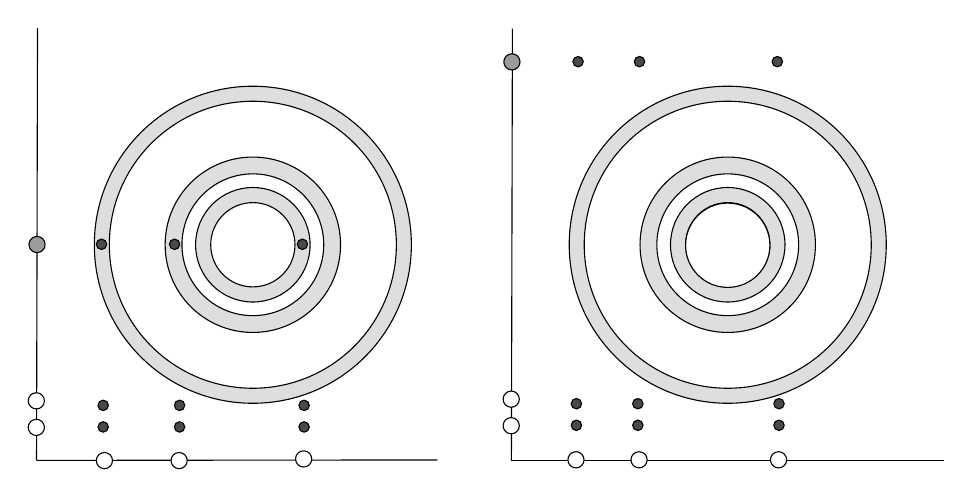
\begin{tikzpicture}[x=0.75pt,y=0.75pt,yscale=0.8,xscale=0.8]
%uncomment if require: \path (0,299); %set diagram left start at 0, and has height of 299

%Straight Lines [id:da8194240959270346] 
\draw    (314,19.7) -- (314.6,279.97) ;
%Straight Lines [id:da12205278341739523] 
\draw    (314,19.7) -- (574.55,19.7) ;
%Straight Lines [id:da8187123168571464] 
\draw    (28,20) -- (269.6,20.27) ;
%Straight Lines [id:da796553864028118] 
\draw    (28,20) -- (28.6,280.27) ;
%Shape: Circle [id:dp7829643160935992] 
\draw  [fill={rgb, 255:red, 222; green, 222; blue, 222 }  ,fill opacity=1 ] (348.81,149.87) .. controls (348.81,97.14) and (391.55,54.4) .. (444.27,54.4) .. controls (497,54.4) and (539.74,97.14) .. (539.74,149.87) .. controls (539.74,202.59) and (497,245.34) .. (444.27,245.34) .. controls (391.55,245.34) and (348.81,202.59) .. (348.81,149.87) -- cycle ;
%Shape: Circle [id:dp3106807534625411] 
\draw  [fill={rgb, 255:red, 255; green, 255; blue, 255 }  ,fill opacity=1 ] (357.85,149.87) .. controls (357.85,102.14) and (396.55,63.45) .. (444.27,63.45) .. controls (492,63.45) and (530.7,102.14) .. (530.7,149.87) .. controls (530.7,197.6) and (492,236.29) .. (444.27,236.29) .. controls (396.55,236.29) and (357.85,197.6) .. (357.85,149.87) -- cycle ;
%Shape: Circle [id:dp30551387107036876] 
\draw  [fill={rgb, 255:red, 222; green, 222; blue, 222 }  ,fill opacity=1 ] (391.46,149.87) .. controls (391.46,120.7) and (415.1,97.05) .. (444.27,97.05) .. controls (473.45,97.05) and (497.09,120.7) .. (497.09,149.87) .. controls (497.09,179.04) and (473.45,202.68) .. (444.27,202.68) .. controls (415.1,202.68) and (391.46,179.04) .. (391.46,149.87) -- cycle ;
%Shape: Circle [id:dp0407471735325019] 
\draw  [fill={rgb, 255:red, 255; green, 255; blue, 255 }  ,fill opacity=1 ] (401.58,149.87) .. controls (401.58,126.29) and (420.7,107.17) .. (444.27,107.17) .. controls (467.85,107.17) and (486.97,126.29) .. (486.97,149.87) .. controls (486.97,173.45) and (467.85,192.56) .. (444.27,192.56) .. controls (420.7,192.56) and (401.58,173.45) .. (401.58,149.87) -- cycle ;
%Shape: Circle [id:dp7794418165975352] 
\draw  [fill={rgb, 255:red, 222; green, 222; blue, 222 }  ,fill opacity=1 ] (409.8,149.87) .. controls (409.8,130.83) and (425.24,115.39) .. (444.27,115.39) .. controls (463.31,115.39) and (478.75,130.83) .. (478.75,149.87) .. controls (478.75,168.91) and (463.31,184.34) .. (444.27,184.34) .. controls (425.24,184.34) and (409.8,168.91) .. (409.8,149.87) -- cycle ;
%Shape: Circle [id:dp8077673979250265] 
\draw  [fill={rgb, 255:red, 255; green, 255; blue, 255 }  ,fill opacity=1 ] (418.9,149.87) .. controls (418.9,135.85) and (430.26,124.49) .. (444.27,124.49) .. controls (458.29,124.49) and (469.65,135.85) .. (469.65,149.87) .. controls (469.65,163.88) and (458.29,175.24) .. (444.27,175.24) .. controls (430.26,175.24) and (418.9,163.88) .. (418.9,149.87) -- cycle ;
%Shape: Circle [id:dp6998803528397256] 
\draw  [fill={rgb, 255:red, 222; green, 222; blue, 222 }  ,fill opacity=1 ] (62.81,149.87) .. controls (62.81,97.14) and (105.55,54.4) .. (158.27,54.4) .. controls (211,54.4) and (253.74,97.14) .. (253.74,149.87) .. controls (253.74,202.59) and (211,245.34) .. (158.27,245.34) .. controls (105.55,245.34) and (62.81,202.59) .. (62.81,149.87) -- cycle ;
%Shape: Circle [id:dp4255421774727244] 
\draw  [fill={rgb, 255:red, 255; green, 255; blue, 255 }  ,fill opacity=1 ] (71.85,149.87) .. controls (71.85,102.14) and (110.55,63.45) .. (158.27,63.45) .. controls (206,63.45) and (244.7,102.14) .. (244.7,149.87) .. controls (244.7,197.6) and (206,236.29) .. (158.27,236.29) .. controls (110.55,236.29) and (71.85,197.6) .. (71.85,149.87) -- cycle ;
%Shape: Circle [id:dp06617638524915026] 
\draw  [fill={rgb, 255:red, 222; green, 222; blue, 222 }  ,fill opacity=1 ] (105.46,149.87) .. controls (105.46,120.7) and (129.1,97.05) .. (158.27,97.05) .. controls (187.45,97.05) and (211.09,120.7) .. (211.09,149.87) .. controls (211.09,179.04) and (187.45,202.68) .. (158.27,202.68) .. controls (129.1,202.68) and (105.46,179.04) .. (105.46,149.87) -- cycle ;
%Shape: Circle [id:dp9352030665686459] 
\draw  [fill={rgb, 255:red, 255; green, 255; blue, 255 }  ,fill opacity=1 ] (115.58,149.87) .. controls (115.58,126.29) and (134.7,107.17) .. (158.27,107.17) .. controls (181.85,107.17) and (200.97,126.29) .. (200.97,149.87) .. controls (200.97,173.45) and (181.85,192.56) .. (158.27,192.56) .. controls (134.7,192.56) and (115.58,173.45) .. (115.58,149.87) -- cycle ;
%Shape: Circle [id:dp17989716938459888] 
\draw  [fill={rgb, 255:red, 222; green, 222; blue, 222 }  ,fill opacity=1 ] (123.8,149.87) .. controls (123.8,130.83) and (139.24,115.39) .. (158.27,115.39) .. controls (177.31,115.39) and (192.75,130.83) .. (192.75,149.87) .. controls (192.75,168.91) and (177.31,184.34) .. (158.27,184.34) .. controls (139.24,184.34) and (123.8,168.91) .. (123.8,149.87) -- cycle ;
%Shape: Circle [id:dp6851632806180186] 
\draw  [fill={rgb, 255:red, 255; green, 255; blue, 255 }  ,fill opacity=1 ] (132.9,149.87) .. controls (132.9,135.85) and (144.26,124.49) .. (158.27,124.49) .. controls (172.29,124.49) and (183.65,135.85) .. (183.65,149.87) .. controls (183.65,163.88) and (172.29,175.24) .. (158.27,175.24) .. controls (144.26,175.24) and (132.9,163.88) .. (132.9,149.87) -- cycle ;
%Shape: Circle [id:dp40350144630782714] 
\draw  [fill={rgb, 255:red, 255; green, 255; blue, 255 }  ,fill opacity=1 ] (64,19.88) .. controls (64,17.18) and (66.18,15) .. (68.88,15) .. controls (71.57,15) and (73.75,17.18) .. (73.75,19.88) .. controls (73.75,22.57) and (71.57,24.75) .. (68.88,24.75) .. controls (66.18,24.75) and (64,22.57) .. (64,19.88) -- cycle ;
%Shape: Circle [id:dp08899969161544696] 
\draw  [fill={rgb, 255:red, 255; green, 255; blue, 255 }  ,fill opacity=1 ] (418.9,149.57) .. controls (418.9,135.55) and (430.26,124.19) .. (444.27,124.19) .. controls (458.29,124.19) and (469.65,135.55) .. (469.65,149.57) .. controls (469.65,163.58) and (458.29,174.94) .. (444.27,174.94) .. controls (430.26,174.94) and (418.9,163.58) .. (418.9,149.57) -- cycle ;
%Shape: Circle [id:dp5743651141366687] 
\draw  [fill={rgb, 255:red, 74; green, 74; blue, 74 }  ,fill opacity=1 ] (64,150.14) .. controls (64,148.41) and (65.41,147) .. (67.14,147) .. controls (68.88,147) and (70.28,148.41) .. (70.28,150.14) .. controls (70.28,151.88) and (68.88,153.28) .. (67.14,153.28) .. controls (65.41,153.28) and (64,151.88) .. (64,150.14) -- cycle ;
%Shape: Circle [id:dp13210263164899094] 
\draw  [fill={rgb, 255:red, 74; green, 74; blue, 74 }  ,fill opacity=1 ] (108,150.14) .. controls (108,148.41) and (109.41,147) .. (111.14,147) .. controls (112.88,147) and (114.28,148.41) .. (114.28,150.14) .. controls (114.28,151.88) and (112.88,153.28) .. (111.14,153.28) .. controls (109.41,153.28) and (108,151.88) .. (108,150.14) -- cycle ;
%Shape: Circle [id:dp74213242291322] 
\draw  [fill={rgb, 255:red, 74; green, 74; blue, 74 }  ,fill opacity=1 ] (185,150.14) .. controls (185,148.41) and (186.41,147) .. (188.14,147) .. controls (189.88,147) and (191.28,148.41) .. (191.28,150.14) .. controls (191.28,151.88) and (189.88,153.28) .. (188.14,153.28) .. controls (186.41,153.28) and (185,151.88) .. (185,150.14) -- cycle ;
%Shape: Circle [id:dp6666612504590449] 
\draw  [fill={rgb, 255:red, 74; green, 74; blue, 74 }  ,fill opacity=1 ] (65,53.14) .. controls (65,51.41) and (66.41,50) .. (68.14,50) .. controls (69.88,50) and (71.28,51.41) .. (71.28,53.14) .. controls (71.28,54.88) and (69.88,56.28) .. (68.14,56.28) .. controls (66.41,56.28) and (65,54.88) .. (65,53.14) -- cycle ;
%Shape: Circle [id:dp25417231201667445] 
\draw  [fill={rgb, 255:red, 74; green, 74; blue, 74 }  ,fill opacity=1 ] (65,40.14) .. controls (65,38.41) and (66.41,37) .. (68.14,37) .. controls (69.88,37) and (71.28,38.41) .. (71.28,40.14) .. controls (71.28,41.88) and (69.88,43.28) .. (68.14,43.28) .. controls (66.41,43.28) and (65,41.88) .. (65,40.14) -- cycle ;
%Shape: Circle [id:dp20816207183269508] 
\draw  [fill={rgb, 255:red, 74; green, 74; blue, 74 }  ,fill opacity=1 ] (111,40.14) .. controls (111,38.41) and (112.41,37) .. (114.14,37) .. controls (115.88,37) and (117.28,38.41) .. (117.28,40.14) .. controls (117.28,41.88) and (115.88,43.28) .. (114.14,43.28) .. controls (112.41,43.28) and (111,41.88) .. (111,40.14) -- cycle ;
%Shape: Circle [id:dp8890493225780333] 
\draw  [fill={rgb, 255:red, 74; green, 74; blue, 74 }  ,fill opacity=1 ] (111,53.14) .. controls (111,51.41) and (112.41,50) .. (114.14,50) .. controls (115.88,50) and (117.28,51.41) .. (117.28,53.14) .. controls (117.28,54.88) and (115.88,56.28) .. (114.14,56.28) .. controls (112.41,56.28) and (111,54.88) .. (111,53.14) -- cycle ;
%Shape: Circle [id:dp7412941805834966] 
\draw  [fill={rgb, 255:red, 74; green, 74; blue, 74 }  ,fill opacity=1 ] (186,53.14) .. controls (186,51.41) and (187.41,50) .. (189.14,50) .. controls (190.88,50) and (192.28,51.41) .. (192.28,53.14) .. controls (192.28,54.88) and (190.88,56.28) .. (189.14,56.28) .. controls (187.41,56.28) and (186,54.88) .. (186,53.14) -- cycle ;
%Shape: Circle [id:dp48065283288266936] 
\draw  [fill={rgb, 255:red, 74; green, 74; blue, 74 }  ,fill opacity=1 ] (186,40.14) .. controls (186,38.41) and (187.41,37) .. (189.14,37) .. controls (190.88,37) and (192.28,38.41) .. (192.28,40.14) .. controls (192.28,41.88) and (190.88,43.28) .. (189.14,43.28) .. controls (187.41,43.28) and (186,41.88) .. (186,40.14) -- cycle ;
%Shape: Circle [id:dp34091589540709266] 
\draw  [fill={rgb, 255:red, 74; green, 74; blue, 74 }  ,fill opacity=1 ] (350,41.14) .. controls (350,39.41) and (351.41,38) .. (353.14,38) .. controls (354.88,38) and (356.28,39.41) .. (356.28,41.14) .. controls (356.28,42.88) and (354.88,44.28) .. (353.14,44.28) .. controls (351.41,44.28) and (350,42.88) .. (350,41.14) -- cycle ;
%Shape: Circle [id:dp8489646709173403] 
\draw  [fill={rgb, 255:red, 74; green, 74; blue, 74 }  ,fill opacity=1 ] (387,41.14) .. controls (387,39.41) and (388.41,38) .. (390.14,38) .. controls (391.88,38) and (393.28,39.41) .. (393.28,41.14) .. controls (393.28,42.88) and (391.88,44.28) .. (390.14,44.28) .. controls (388.41,44.28) and (387,42.88) .. (387,41.14) -- cycle ;
%Shape: Circle [id:dp311004704357545] 
\draw  [fill={rgb, 255:red, 74; green, 74; blue, 74 }  ,fill opacity=1 ] (472,41.14) .. controls (472,39.41) and (473.41,38) .. (475.14,38) .. controls (476.88,38) and (478.28,39.41) .. (478.28,41.14) .. controls (478.28,42.88) and (476.88,44.28) .. (475.14,44.28) .. controls (473.41,44.28) and (472,42.88) .. (472,41.14) -- cycle ;
%Shape: Circle [id:dp31170134224605195] 
\draw  [fill={rgb, 255:red, 74; green, 74; blue, 74 }  ,fill opacity=1 ] (350,54.14) .. controls (350,52.41) and (351.41,51) .. (353.14,51) .. controls (354.88,51) and (356.28,52.41) .. (356.28,54.14) .. controls (356.28,55.88) and (354.88,57.28) .. (353.14,57.28) .. controls (351.41,57.28) and (350,55.88) .. (350,54.14) -- cycle ;
%Shape: Circle [id:dp28532980461694424] 
\draw  [fill={rgb, 255:red, 74; green, 74; blue, 74 }  ,fill opacity=1 ] (387,54.14) .. controls (387,52.41) and (388.41,51) .. (390.14,51) .. controls (391.88,51) and (393.28,52.41) .. (393.28,54.14) .. controls (393.28,55.88) and (391.88,57.28) .. (390.14,57.28) .. controls (388.41,57.28) and (387,55.88) .. (387,54.14) -- cycle ;
%Shape: Circle [id:dp6020013292698594] 
\draw  [fill={rgb, 255:red, 74; green, 74; blue, 74 }  ,fill opacity=1 ] (472,54.14) .. controls (472,52.41) and (473.41,51) .. (475.14,51) .. controls (476.88,51) and (478.28,52.41) .. (478.28,54.14) .. controls (478.28,55.88) and (476.88,57.28) .. (475.14,57.28) .. controls (473.41,57.28) and (472,55.88) .. (472,54.14) -- cycle ;
%Shape: Circle [id:dp023435344947860814] 
\draw  [fill={rgb, 255:red, 74; green, 74; blue, 74 }  ,fill opacity=1 ] (351,260.14) .. controls (351,258.41) and (352.41,257) .. (354.14,257) .. controls (355.88,257) and (357.28,258.41) .. (357.28,260.14) .. controls (357.28,261.88) and (355.88,263.28) .. (354.14,263.28) .. controls (352.41,263.28) and (351,261.88) .. (351,260.14) -- cycle ;
%Shape: Circle [id:dp781542616798407] 
\draw  [fill={rgb, 255:red, 74; green, 74; blue, 74 }  ,fill opacity=1 ] (388,260.14) .. controls (388,258.41) and (389.41,257) .. (391.14,257) .. controls (392.88,257) and (394.28,258.41) .. (394.28,260.14) .. controls (394.28,261.88) and (392.88,263.28) .. (391.14,263.28) .. controls (389.41,263.28) and (388,261.88) .. (388,260.14) -- cycle ;
%Shape: Circle [id:dp7192093882668958] 
\draw  [fill={rgb, 255:red, 74; green, 74; blue, 74 }  ,fill opacity=1 ] (471,260.14) .. controls (471,258.41) and (472.41,257) .. (474.14,257) .. controls (475.88,257) and (477.28,258.41) .. (477.28,260.14) .. controls (477.28,261.88) and (475.88,263.28) .. (474.14,263.28) .. controls (472.41,263.28) and (471,261.88) .. (471,260.14) -- cycle ;
%Shape: Circle [id:dp08487765818129678] 
\draw  [fill={rgb, 255:red, 255; green, 255; blue, 255 }  ,fill opacity=1 ] (109,19.88) .. controls (109,17.18) and (111.18,15) .. (113.88,15) .. controls (116.57,15) and (118.75,17.18) .. (118.75,19.88) .. controls (118.75,22.57) and (116.57,24.75) .. (113.88,24.75) .. controls (111.18,24.75) and (109,22.57) .. (109,19.88) -- cycle ;
%Shape: Circle [id:dp7550770077214879] 
\draw  [fill={rgb, 255:red, 255; green, 255; blue, 255 }  ,fill opacity=1 ] (184,20.88) .. controls (184,18.18) and (186.18,16) .. (188.88,16) .. controls (191.57,16) and (193.75,18.18) .. (193.75,20.88) .. controls (193.75,23.57) and (191.57,25.75) .. (188.88,25.75) .. controls (186.18,25.75) and (184,23.57) .. (184,20.88) -- cycle ;
%Shape: Circle [id:dp011014467225936797] 
\draw  [fill={rgb, 255:red, 255; green, 255; blue, 255 }  ,fill opacity=1 ] (23,39.88) .. controls (23,37.18) and (25.18,35) .. (27.88,35) .. controls (30.57,35) and (32.75,37.18) .. (32.75,39.88) .. controls (32.75,42.57) and (30.57,44.75) .. (27.88,44.75) .. controls (25.18,44.75) and (23,42.57) .. (23,39.88) -- cycle ;
%Shape: Circle [id:dp9016398775074254] 
\draw  [fill={rgb, 255:red, 255; green, 255; blue, 255 }  ,fill opacity=1 ] (23,55.88) .. controls (23,53.18) and (25.18,51) .. (27.88,51) .. controls (30.57,51) and (32.75,53.18) .. (32.75,55.88) .. controls (32.75,58.57) and (30.57,60.75) .. (27.88,60.75) .. controls (25.18,60.75) and (23,58.57) .. (23,55.88) -- cycle ;
%Shape: Circle [id:dp5891247736437845] 
\draw  [fill={rgb, 255:red, 155; green, 155; blue, 155 }  ,fill opacity=1 ] (23.43,150.01) .. controls (23.43,147.32) and (25.61,145.13) .. (28.3,145.13) .. controls (30.99,145.13) and (33.18,147.32) .. (33.18,150.01) .. controls (33.18,152.7) and (30.99,154.88) .. (28.3,154.88) .. controls (25.61,154.88) and (23.43,152.7) .. (23.43,150.01) -- cycle ;
%Shape: Circle [id:dp5966776679620737] 
\draw  [fill={rgb, 255:red, 255; green, 255; blue, 255 }  ,fill opacity=1 ] (348,20.36) .. controls (348,17.67) and (350.18,15.48) .. (352.88,15.48) .. controls (355.57,15.48) and (357.75,17.67) .. (357.75,20.36) .. controls (357.75,23.05) and (355.57,25.23) .. (352.88,25.23) .. controls (350.18,25.23) and (348,23.05) .. (348,20.36) -- cycle ;
%Shape: Circle [id:dp7740110171501559] 
\draw  [fill={rgb, 255:red, 255; green, 255; blue, 255 }  ,fill opacity=1 ] (386,20.36) .. controls (386,17.67) and (388.18,15.48) .. (390.88,15.48) .. controls (393.57,15.48) and (395.75,17.67) .. (395.75,20.36) .. controls (395.75,23.05) and (393.57,25.23) .. (390.88,25.23) .. controls (388.18,25.23) and (386,23.05) .. (386,20.36) -- cycle ;
%Shape: Circle [id:dp6095822005010809] 
\draw  [fill={rgb, 255:red, 255; green, 255; blue, 255 }  ,fill opacity=1 ] (470,20.36) .. controls (470,17.67) and (472.18,15.48) .. (474.88,15.48) .. controls (477.57,15.48) and (479.75,17.67) .. (479.75,20.36) .. controls (479.75,23.05) and (477.57,25.23) .. (474.88,25.23) .. controls (472.18,25.23) and (470,23.05) .. (470,20.36) -- cycle ;
%Shape: Circle [id:dp7682016765751116] 
\draw  [fill={rgb, 255:red, 255; green, 255; blue, 255 }  ,fill opacity=1 ] (309,40.88) .. controls (309,38.18) and (311.18,36) .. (313.88,36) .. controls (316.57,36) and (318.75,38.18) .. (318.75,40.88) .. controls (318.75,43.57) and (316.57,45.75) .. (313.88,45.75) .. controls (311.18,45.75) and (309,43.57) .. (309,40.88) -- cycle ;
%Shape: Circle [id:dp7837323222556574] 
\draw  [fill={rgb, 255:red, 255; green, 255; blue, 255 }  ,fill opacity=1 ] (309,56.88) .. controls (309,54.18) and (311.18,52) .. (313.88,52) .. controls (316.57,52) and (318.75,54.18) .. (318.75,56.88) .. controls (318.75,59.57) and (316.57,61.75) .. (313.88,61.75) .. controls (311.18,61.75) and (309,59.57) .. (309,56.88) -- cycle ;
%Shape: Circle [id:dp030269638935122578] 
\draw  [fill={rgb, 255:red, 155; green, 155; blue, 155 }  ,fill opacity=1 ] (309.43,260.01) .. controls (309.43,257.32) and (311.61,255.13) .. (314.3,255.13) .. controls (316.99,255.13) and (319.18,257.32) .. (319.18,260.01) .. controls (319.18,262.7) and (316.99,264.88) .. (314.3,264.88) .. controls (311.61,264.88) and (309.43,262.7) .. (309.43,260.01) -- cycle ;




\end{tikzpicture}




\caption{The two diagrams displayed indicate two instances of the process of defining the set $S$ for the function $f(x_1,x_2) = x_1^2 + x_2^2$. Here $K = 3$, $n = 3$, the values on the $x$-axis represent the values $X_1(1), X_1(2),$ and $X_1(3)$, the values on the $y$-axis represent the values $X_2(1), X_2(2)$, and $X_2(3)$, the dark points represent the family of all pairs $(X_1(k_1),X_2(k_2))$, and the annuli represent the $r$-neighborhoods of $f^{-1}(X_3(1)), f^{-1}(X_3(2))$, and $f^{-1}(X_3(3))$. In the left diagram, $S = \{ 1,2,3 \}$, whereas in the right diagram $S = \emptyset$. Thus $S$ can be completely changed simply by adjusting the position of the shaded point on the $y$-axis (adjusting one of the variables $X_2(k)$), which completely changes the value of $\widehat{\sigma}$. Nonetheless, this only occurs if the other values are arranged in a highly particular manner.}
\label{thefigure}
\end{center}
\end{figure}

\begin{remark}
    Before we begin the proof of this lemma, let us describe the idea of the proof. As a random quantity, $\widehat{\sigma}(\xi)$ is a function of the independent random quantities $\{ X_i(k) \}$, and so McDiarmid's inequality presents itself as a useful concentration bound. However, a naive application of McDiarmid's inequality fails here, because changing a single random variable $X_i(k)$ for $1 \leq i \leq n-1$ while fixing all other random variables can change $\widehat{\sigma}(\xi)$ by as much as $O(1)$ (see Figure \ref{thefigure}), which is far too much to obtain the square root cancellation bounds like we obtained in \eqref{equationCOIACOIAJCPPPPP}. On the other hand, it seems that a single variable $X_i(k)$ only changes $\widehat{\sigma}(\xi)$ by $O(1)$ if the random variables $\{ X_1(k) \}$ are configured in a very particular way, which is unlikely to happen. Thus we should expect that adjusting a single random variable $X_i(k)$ does not influence the value of $\widehat{\sigma}(\xi)$ very much if the quantity $\widehat{\sigma}(\xi)$ is \emph{averaged} over the possible choices of $\{ X_1(k) \}$, and then we can apply McDiarmid's inequality.
\end{remark}

\begin{proof}
    Consider the random set $\Omega$ of values $x_n \in Q_n$ such that there are $k_1,\dots,k_{n-1} \in \{ 1,\dots,K \}$ with
    %
    \begin{equation}
        |x_n - f(X_1(k_1),\dots,X_{n-1}(k_{n-1}))| \leq (L+1)r.
    \end{equation}
    %
    Then
    %
    \begin{equation}
        \widehat{\sigma}(\xi) = \frac{1}{K} \sum_{k = 1}^K Z(k).
    \end{equation}
    %
    where
    %
    \[ Z(k) = \begin{cases} e^{2 \pi i \xi \cdot X_n(k)} &: X_n(k) \in \Omega, \\ 0 &: X_n(k) \not \in \Omega \end{cases}. \]
    %
    If $\Sigma$ is the $\sigma$ algebra generated by the random variables
    %
    \[ \{ X_i(k) : i \in \{ 1, \dots, n-1 \}, k \in \{ 1, \dots, K \} \}, \]
    %
    then the random variables $\{ Z(k) \}$ are \emph{conditionally independent} given $\Sigma$. Since we have $|Z(k)| \leq 1$ almost surely, Hoeffding's inequality thus implies that for all $t \geq 0$,
    %
    \begin{equation} \label{equationCOIJCOIJX1232312}
        \PP \left( \left| \widehat{\sigma}(\xi) - \EE(\widehat{\sigma}(\xi)|\Sigma) \right| \geq t \right) \leq 4 \exp \left( \frac{-K t^2}{2} \right).
    \end{equation}
    %
    It is simple to see that
    %
    \begin{equation}
        \EE(\widehat{\sigma}(\xi) | \Sigma) = \int_\Omega \psi_n(x) e^{2 \pi i \xi \cdot x}\; dx.
    \end{equation}
    %
    Since
    %
    \begin{equation}
        \Omega = \bigcup \left\{ B_r(f(X_1(k_1),\dots,X_{n-1}(k_{n-1}))) : 1 \leq k_1,\dots,k_{n-1} \leq K \right\}.
    \end{equation}
    % K^{n-1} = r^{(n-1) \varepsilon_1/2 - d}
    we see that varying each random variable $X_i(k)$, for $1 \leq i \leq n-1$ which fixing the other random variables adjusts at most $K^{n-2}$ of the radius $r$ balls forming $\Omega$, and thus varying $X_i(k)$ independently of the other random variables changes $\EE(\widehat{\sigma}(\xi)|\Sigma)$ by at most
    %
    \begin{equation}
        2 \cdot (2r)^d \cdot K^{n-2} = 2^{d+1} \cdot r^d \cdot K^{n-2} \leq \frac{2^{d+1}}{K} \leq \frac{2^{d+1}}{K}.
    \end{equation}
    % K^{-(n-1)} = r^d
    % 
    Thus McDiarmid's inequality shows that for any $t \geq 0$,
    %
    \begin{equation} \label{equationCIJCIJIVJIO}
        \PP \left( |\EE(\widehat{\sigma}(\xi)|\Sigma) - \EE(\widehat{\sigma}(\xi))| \geq t \right) \leq 4 \exp \left( \frac{-K t^2}{2^{2d+1}} \right).
    \end{equation}
    %
    Combining \eqref{equationCOIJCOIJX1232312} and \eqref{equationCIJCIJIVJIO}, we conclude that for each $\xi \in \ZZ^d$,
    %
    \begin{equation} \label{equationCNCIJIJOJOPPPPOPODAW}
        \PP \left( | \widehat{\sigma}(\xi) - \EE(\widehat{\sigma}(\xi)) | \geq t  \right) \leq 8 \exp \left( \frac{-K t^2}{2^{2d + 1}} \right).
    \end{equation}
    %
    Applying a union bound to \eqref{equationCNCIJIJOJOPPPPOPODAW} over all $\xi \in B$ shows that there exists a constant $C > 0$ such that
    %
    \[ \PP \left( \| \widehat{\sigma}(\xi) - \EE(\widehat{\sigma}(\xi)) \|_{L^\infty(B)} \geq C K^{-1/2} \log(K)^{1/2} \right) \leq 1/10. \qedhere \]
\end{proof}

The analysis of \eqref{equationCIJCIJIJXSO} requires a more technical calculation.

\begin{lemma} \label{lemmaOIJIOCJSOIJSIOJ123}
    Let $\sigma$ be the random measure described in Lemma \ref{lemmaOIOICJOIJOISJOIJS}. Then there exists $C > 0$ such that for any $\delta > 0$, there exists $r_0 > 0$ such that for $r \leq r_0$,
    %
    \[ |\EE(\widehat{\sigma}(\xi))| \leq CK^{-1/2} + \delta |\xi|^{-\beta/2}. \]
\end{lemma}
\begin{proof}
    We break the analysis of $\EE(\widehat{\sigma}(\xi))$ into two cases, depending on whether $n = 2$ or $n > 2$. The major difference here is that when $n > 2$, $\beta < d$, whereas when $n = 2$, $\beta = d$, i.e.  we are constructing a full dimensional set,  so that some argument that work for the case $n > 2$ fail when $n = 2$. On the other hand, the analysis of patterns when $n = 2$ is more trivial than the analysis for $n > 2$, which makes this argument more simple in other respects.
%    \[ \PP(1 \in S) \EE(e^{2 \pi i \xi \cdot X_1} | 1 \in S) = K^n \]
%    \[ \PP(1 \in S) = O(1) \] % K^{n-1} radius r balls, thus having total measure $(r^e) Doesn't Help us. But if the function is locally constant, it does help us.
%    \[ \EE(e^{2 \pi i \xi \cdot X_1} | 1 \in S) \]
    % Provided this is smooth this will give arbitrary decay. If this isn't smooth, then the function is probably roughly constant so the other term gives good bounds.
%
%    Given a set $E \subset \TT^{d(n-1)}$, what is
    %
%    \[ \PP \left( (X_2(k_2),\dots,X_n(k_n)) \in E\ \text{for some $1 \leq k_2,\dots,k_n \leq K$} \right) \]
    %
%    This should be proportional to $|E|$, but the calculation is more difficult than for the expectation bound on the number of such indices. Can we view this as a kind of multilinear function of the variables $\{ X_i(k_i) \}$ so we can apply decoupling? The event we are analyzing is
    %
%    \[ \EE \left( 1 - \prod_{k_2,\dots,k_n} \left[ 1 - \mathbf{I}((X_2(k_2),\dots,X_n(k_n)) \in E) \right] \right) \]
    %
%    vs.
    %
%    \[ \EE \left( \sum_{k_2,\dots,k_n} \mathbf{I}((X_2(k_2),\dots,X_n(k_n)) \in E) \right) = K^{n-1} |E| \approx 1 \]
    %
%    so independence is much more important in the top version.
%
%    If each sample was independant, then the top value would be equal to
    % |E| is an r thickening of a manifold of dimension d(n-2) in R^{d(n-1)} so
%    \[ 1 - ( 1 - |E| )^{K^n} = 1 - \left( (1 - 1/K^{n-1})^{K^{n-1}} \right)^K \approx 1 - e^{-K} \]
%
%
%    What if the set was
    %
%    \[ \PP( X_2(k_2) = g(X_3(k_3),\dots,X_n(k_n))\ \text{for some $1 \leq k_2,\dots,k_n \leq K$} ) \]

%    For each $k \in \{ 1, \dots, K \}$, the density of $X_1(k)$ given that $k \in S$ at $x \in \TT^d$ should be
    %
%    \[ K^{n-1} \int_W \int_{B_{(L+1)r}(0)} \psi(x,x_2,\dots,x_k) \]

    %
%    \[ \EE( e^{2 \pi i \xi \cdot X_1(k)} \mathbf{I}(k \in S) ) = \PP(k \in S) \EE \left( e^{2 \pi i X_1(k)} | k \in S \right) \]

    Let's start with the case $n = 2$. Using the fact that the family $\{ X_n(k) : 1 \leq k \leq K \}$ are uniformly distributed, we calculate that
    %
    \begin{equation} \label{equationDJACIOJCOWIJ}
    \begin{split}
        \EE(\widehat{\sigma}(\xi)) &= \EE ( A_2 \cdot e^{2 \pi i \xi \cdot X_2(1)} \cdot \mathbf{I}(1 \in S) )\\
        &= A_2 \int_{\TT^d} \psi_2(x) \PP \left( 1 \in S | X_2(1) = x \right) e^{2 \pi i \xi \cdot x}\; dx.
    \end{split}
    \end{equation}
    %
    For each $x \in \TT^d$, a change of variables formula implies that
    %
    \begin{equation}
    \begin{split}
        \PP(1 \in S | X_1(1) = x) &= 1 - \left( 1 - \int_{f^{-1}(B_{(L+1)r}(x))} \psi_1(x_1)\; dx_1 \right)^K\\
        &= 1 - \left( 1 - \int_{B_{(L+1) r}(x)} \frac{(\psi_1 \circ f^{-1})(x_2)}{|\det(Df)(f^{-1}(x_2))|}\; dx_2 \right)^K\\
        &= 1 - \left( 1 - \int_{B_{(L+1)r}(x)} \tilde{\psi_1}(x_2)\; dx_2 \right)^K,
    \end{split}
    \end{equation}
    %
    where we have introduced $\tilde{\psi_1}$ for notational convenience. If we define
    %
    \[ g(x) = \PP(1 \in S| X_1(1) = x), \]
    %
    then $\EE(\widehat{\sigma}(\xi)) = A_2 \cdot \widehat{\psi_2 g}(\xi)$. We can obtain a bound on this quantity by bounding the partial derivatives of $\psi_2 g$. Bernoulli's inequality implies that
    %
    \begin{equation}
        g(x) = 1 - \left( 1 - \int_{B_{(L+1)r}} \tilde{\psi_1}(x_2)\; dx_2 \right)^K \lesssim_L K r^d \leq r^{\varepsilon_1/2}.
    \end{equation}
    %
    On the other hand, if $\alpha > 0$, then $\partial_\alpha g(x)$ is a sum of terms of the form
    %
    \begin{equation} \label{equationDOIJACOIJCIOJ3123123214312}
        (-1)^m \frac{K!}{(K-m)!} \left( 1 - \int_{B_{(L+1) r}(x)} \tilde{\psi_1}(x_2)\; dx_2 \right)^{K-m} \left( \prod_{i = 1}^{m} \int_{B_{(L+1)r}(x)} \partial_{\alpha_i} \tilde{\psi_1}(x_2)\; dx_2 \right),
    \end{equation}
    %
    where $\alpha_i \neq 0$ for any $i$ and $\alpha = \alpha_1 + \dots + \alpha_m$. This implies $0 < m \leq |\alpha|$ for any terms in the sum. Now the bound $|\partial_{\alpha_i} \tilde{\psi_1}(x_2)| \lesssim_{\alpha_i} 1$ implies that
    %
    \begin{equation} \label{equationDOIAJCOIJAWCIOJAWOIJWAOI}
        \left| \int_{B_{(L+1)r}(x)} \partial_{\alpha_i} \tilde{\psi_1}(x_2)\; dx_2 \right| \lesssim_{\alpha_i} r^d.
    \end{equation}
    %
    Applying \eqref{equationDOIAJCOIJAWCIOJAWOIJWAOI} to \eqref{equationDOIJACOIJCIOJ3123123214312} enables us to conclude that
    %
    \begin{equation} \label{equationIOJACIOAJCOIWAJ}
        |\partial_\alpha g(x)| \lesssim_\alpha \max_{m \leq |\alpha|} K^m r^{md} \leq r^{\varepsilon_1/2},
    \end{equation}
    %
    Since the fact that $\psi_2 \in C^\infty(\mathbf{T}^d)$ implies that $\| \partial_\alpha \psi_2 \|_{L^\infty(\TT^d)} \lesssim_\alpha 1$ for any multi-index $\alpha$, the product rule applied to \eqref{equationIOJACIOAJCOIWAJ} implies that $\| \partial_\alpha (\psi_2 g) \|_{L^\infty(\TT^d)} \lesssim_\alpha r^{\varepsilon_1/2}$ for all $\alpha > 0$, which means that for any $N > 0$ and $\xi \neq 0$,
    %
    \begin{equation} \label{equationCIOCIJIXJIXJI}
        |\EE(\widehat{\sigma}(\xi))| \lesssim_N r^{\varepsilon_1/2} |\xi|^{-N}.
    \end{equation}
    %
    In particular, setting $N = \beta/2$, fixing $\delta > 0$, and then choosing $r_0$ appropriately, \eqref{equationCIOCIJIXJIXJI} shows that for $r \leq r_0$,
    %
    \begin{equation}
        |\EE(\widehat{\sigma}(\xi))| \leq \delta |\xi|^{-\beta/2}.
    \end{equation}
    %
    This completes the proof in the case $n = 2$.

    Now we move on to the case $n \geq 3$. A version of equation \eqref{equationDJACIOJCOWIJ} continues to hold in this setting, namely that
    %
    \begin{equation} \label{equationGGIJICJIjjpopwaowarr}
        \EE(\widehat{\sigma}(\xi)) = A_n \int_{\TT^d} \psi_n(x) \PP(1 \in S| X_n(1) = x_n) e^{2 \pi i \xi \cdot x_n}\; dx_n.
    \end{equation}
    %
    However, the analysis of this equation is made more complicated by the lack of an explicit formula for $\PP(1 \in S|X_n(1) = x)$. For a set $E \subset \TT^{d(n-1)}$, let $A(E)$ denote the event that there exists $k_1,\dots,k_{n-1}$ such that $(X_1(k_1),\dots,X_{n-1}(k_{n-1})) \in E$. Then
    %
    \begin{equation}
        \PP( 1 \in S | X_1(1) = x ) = \PP(A(f^{-1}(B_{(L+1)r}(x_n)))).
    \end{equation}
    %
    For any cube $Q \in \TT^{d(n-1)}$ and any indices $1 \leq k_1,\dots,k_{n-1} \leq K$, set $k = (k_1,\dots,k_{n-1})$ and let $A(Q;k)$ denote the event that $(X_1(k_1),\dots,X_{n-1}(k_{n-1})) \in Q$. Then
    %
    \[ A(Q) = \bigcup_k A(Q;k). \]
    %
    For any cube $Q$ and index $k$,
    %
    \begin{equation}
        \PP(A(Q;k)) = \int_Q \psi_1(x_1) \dots \psi_{n-1}(x_{n-1})\; dx_1 \dots dx_{n-1},
    \end{equation}
    %
    and so
    %
    \begin{equation} \label{equationOIJCOIJOCIJOAIJOIJAWD}
        \sum_k \PP(A(Q;k)) = K^{n-1} \int_Q \psi_1(x_1) \cdots \psi_{n-1}(x_{n-1})\; dx_1 \dots dx_{n-1}.
    \end{equation}
    %
    An application of inclusion exclusion to \eqref{equationOIJCOIJOCIJOAIJOIJAWD} thus shows that
    %
    \begin{equation} \label{equationIOJVOIVJOVIJPSPOPCOISAPCOIACC}
    \begin{split}
        &\left| \PP(A(Q)) - K^{n-1} \int_Q \psi_1(x_1) \cdots \psi_{n-1}(x_{n-1})\; dx_1 \dots dx_{n-1} \right|\\
        &\quad\quad\quad\leq \sum_{k \neq k'} \PP(A(Q;k) \cap A(Q;k')).
    \end{split}
    \end{equation}
    %
    For each $k,k'$, the quantity $\PP(A(Q;k) \cap A(Q;k'))$ depends on the number of indices $i$ such that $k_i = k_i'$. In particular, if $I \subset \{ 1, \dots, n-1 \}$ is the set of indices where the quantity agrees, then
    %
    \begin{equation}
    \begin{split}
        \PP(A(Q;k) \cap A(Q;k')) = \left( \prod_{i \in I} \int_{Q_i} \psi_i(x)\; dx \right) \cdot \left( \prod_{i \not \in I} \left( \int_{Q_i} \psi_i(x)\; dx \right)^2 \right).
    \end{split}
    \end{equation}
    %
    In particular, if $Q$ has sidelength $l$ and $\#(I) = m$, then $\PP(A(Q;k) \cap A(Q;k')) \lesssim l^{d(2n - m - 2)}$. For each $m$, there are at most $K^{2n - m - 2}$ pairs $k$ and $k'$ with $\#(I) = m$. And so provided $l^d \leq 1/K$,
    %
    \begin{equation} \label{equationCIOJIOJIJCS312412412}
        \sum_{k \neq k'} \PP(A(Q;k) \cap A(Q;k')) \lesssim \sum_{m = 0}^{n-2} (Kl^d)^{2n-m-2} \lesssim K^n l^{dn}.
    \end{equation}
    %
    Thus we conclude from \eqref{equationIOJVOIVJOVIJPSPOPCOISAPCOIACC} and \eqref{equationCIOJIOJIJCS312412412} that
    %
    \begin{equation} \label{equationCIOJOIJXOISJOIj}
        \PP(A(Q)) = K^{n-1} \int_Q \psi_1(x_1) \dots \psi_{n-1}(x_{n-1}) dx_1 \dots dx_{n-1} + O(K^n l^{dn}).
    \end{equation}
    %
    For a particular $x_n \in \TT^d$, let $E = f^{-1}(B_{(L+1)r}(x_n))$. Since $f$ is a submersion, $E$ is contained in a $O(r)$-thickening of a $d(n-2)$ dimensional surface in $\TT^{d(n-1)}$. Applying the Whitney covering lemma, we can find a family of almost disjoint dyadic cubes $\{ Q_{ij} : j \geq 0 \}$ such that
    %
    \begin{equation} \label{equationCOIJIOVJVIVIVIII2231}
        E = \bigcup_{i = 0}^\infty \bigcup_{j = 1}^{n_i} Q_{ij},
    \end{equation}
    %
    where for each $i \geq 0$, $Q_{ij}$ is a sidelength $r/2^i$ cube, and $n_i \lesssim (r/2^i)^{-d(n-2)}$. It follows from \eqref{equationCOIJIOVJVIVIVIII2231} that
    %
    \begin{equation} \label{equationCOJIAWOIJCAWOIJOI}
        A(E) = \bigcup_{i,j} A(Q_{ij}).
    \end{equation}
    %
    Since $n \geq 3$, we can use \eqref{equationCIOJOIJXOISJOIj} to calculate that
    %
    \begin{equation} \label{equationCOIJCOIJSI}
    \begin{split}
        &\left| \sum_{i,j} \PP(A(Q_{ij})) - K^{n-1} \int_E \psi_1(x_1) \dots \psi_{n-1}(x_{n-1})\; dx \right|\\
        &\quad\quad\quad\lesssim \sum_{i = 0}^\infty (r/2^i)^{-d(n-2)} \cdot \left( K^n (r/2^i)^{dn} \right)\\
        &\quad\quad\quad\lesssim r^{2d} K^n \leq K^{-1/2}.
    \end{split}
    \end{equation}
    % r \leq 1/K^{(n/2 + 1/4)/d}
    Thus an inclusion exclusion bound together with \eqref{equationCOJIAWOIJCAWOIJOI} and \eqref{equationCOIJCOIJSI} implies that
    %
    \begin{equation} \label{equationvVIDJDIJ21312ffijsijds}
    \begin{split}
        &\Big| \PP(A(E)) - K^{n-1} \int_E \psi_1(x_1) \dots \psi_{n-1}(x_{n-1})\; dx \Big|\\
        &\quad\quad\quad \lesssim K^{-1/2} + \sum_{(i_1,j_1) \neq (i_2,j_2)} \PP(A(Q_{i_1j_1}) \cap A(Q_{i_2j_2})).
    \end{split}
    \end{equation}
    %
    The quantity $\PP(A(Q_{i_1j_1}) \cap A(Q_{i_2j_2}))$ depends on the relation between the various sides of $Q_{i_1j_1}$ and $Q_{i_2j_2}$. Without loss of generality, we may assume that $i_1 \geq i_2$. If $I(Q_{i_1j_1},Q_{i_2j_2})$ is the set of indices $1 \leq k \leq n-1$ where $Q_{i_1j_1k} \subset Q_{i_2j_2k}$, and $\#(I(Q_{i_1j_1}, Q_{i_2j_2})) = m$, then
    %
    \begin{equation} \label{equationVOIJVIJISJCISJCIEWJRIJI43234}
    \begin{split}
        \PP(A(Q_{i_1j_1}) \cap A(Q_{i_2j_2})) &\lesssim (K(r/2^{i_1})^d)^m \cdot (K(r/2^{i_1})^d \cdot K(r/2^{i_2})^d)^{n-m-1}\\
        &= 2^{-d[(n-1)i_1 + (n-m-1)i_2]} (Kr^d)^{2n - m-2}.
    \end{split}
    \end{equation}
    %
%    \[ \PP(A(Q) \cap A(Q')) = \prod_{i \in I} B_i(Q_i) \cdot \prod_{i \not \in I} C_i(Q_i) \]
    %
%    where
    %
%    \[ B_i(Q_i) = 1 - \left(1 - \int_{Q_i} \psi_i(x)\; dx \right)^K \]
    %
%    and
%    \[ C_i(Q_i) = 1 - \left( 1 - \int_{Q_i} \psi_i(x)\; dx \right)^K - \left( 1 - \int_{Q_i'} \psi_i(x)\; dx \right)^K + \left( 1 - \int_{Q_i \cup Q_i'} \psi_i(x)\; dx \right)^K. \]
    %
%    Then $|B_i(Q_i)| \lesssim K r^d$ and $|C_i(Q_i)| \lesssim K^2 r^{2d}$. If $\#(I) = m$, then we would conclude that $\PP(A(Q) \cap A(Q')) \lesssim K^{2n-m-2} r^{d(2n - m-2)}$.
    The condition that $D_{x_k} f$ is invertible for all $k$ on the domain of $f$ implies that any axis-oriented plane in $\TT^{dn}$ intersects transversally with the level sets of $f$. In particular, this means that the intersection of a $O(r/2^{i_1})$ thickening of a codimension $dm$ axis-oriented hyperplane intersects a $O(r/2^{i_1})$ thickening of $\partial E$ (which has codimension $d$) in a set with volume $O \left( (r/2^{i_1})^d (r/2^{i_1})^{dm} \right)$, and intersects a $O(r/2^{i_2})$ thickening of $\partial E$ in a set with volume $O \left( (r/2^{i_2})^d (r/2^{i_1})^{dm} \right)$. As a particular example of this, for any distinct indices $j_1,\dots,j_m \in \{ 1,\dots, n-1 \}$, and any family of integers $0 \leq n_{11},\dots,n_{md} \leq 2^{i_1}/r$, the set
    %
    \begin{equation}
        \left\{ x \in E : \frac{n_{11}}{2^{i_1}} \leq x_{j_1 1} \leq \frac{(n_{11} + 1)}{2^{i_1}}, \dots, \frac{n_{md}}{2^{i_1}} \leq x_{j_m d} \leq \frac{n_{md} + 1}{2^{i_1}} \right\}
    \end{equation}
    %
    contains at most
    %
    \begin{equation} \label{equationCOIJCOIJSOIJIOJ424141241}
        O \left( (r/2^{i_1})^d (r/2^{i_1})^{dm} (r/2^{i_1})^{-d(n-1)} \right) = O \left( 2^{d(n-m-2)i_1} r^{-d(n-m-2)} \right)
    \end{equation}
    %
    sidelength $r/2^{i_1}$ dyadic cubes in the decomposition of $E$, and at most
    %
    \begin{equation} \label{equationVOIJVOIJVOIJPOPOJP1212312}
        O \left( (r/2^{i_2})^d (r/2^{i_1})^{dm} (r/2^{i_2})^{-d(n-1)} \right) = O \left( 2^{d(n-2) i_2 - (dm) i_1} r^{-d(n-m-2)} \right)
    \end{equation}
    %
    sidelength $r/2^{i_2}$ dyadic cubes in the decomposition of $E$. Letting the integers $\{ n_{kl} \}$ vary over all possible choices we conclude from \eqref{equationCOIJCOIJSOIJIOJ424141241} and \eqref{equationVOIJVOIJVOIJPOPOJP1212312} that for each $i_1$ and $i_2$ there are at most
    %
    \begin{equation} \label{equationCOIJCOIJSOIJOIJ241240912490124091}
    \begin{split}
        &O \left( (2^{i_1}/r)^{dm} \left( 2^{d(n-m-2)i_1} r^{-d(n-m-2)} \right) \left( 2^{d(n-2) i_2 - (dm) i_1} r^{-d(n-m-2)} \right) \right)\\
        &\quad\quad = O \left( 2^{d(n - m - 2)i_1 + d(n-2) i_2} r^{-d(2n - m - 4)} \right)
    \end{split}
    \end{equation}
    %
    pairs $Q_{i_1j_1}$ and $Q_{i_2j_2}$ with $I(Q_{i_1j_1},Q_{i_2j_2}) = m$. Thus we conclude from \eqref{equationVOIJVIJISJCISJCIEWJRIJI43234} and \eqref{equationCOIJCOIJSOIJOIJ241240912490124091} that
    %
    \begin{equation} \label{equationPPOPOKPOPPPPPPDSDSD}
    \begin{split}
        \sum_{(i,j) \neq (i',j')}& \PP(A(Q_{ij}) \cap A(Q_{i'j'}))\\
        &\lesssim \sum_{m = 0}^{n-2} \sum_{i_1 \geq i_2} \left( 2^{d(n-m-2) i_1 + d(n-2) i_2} r^{-d(2n-m-4)} \right)\\
        &\quad\quad\quad\quad\quad\quad\quad\quad\left( 2^{-d((n-1)i_1 + (n-m-1) i_2)} (Kr^d)^{2n - m - 2} \right)\\
        &\lesssim r^{2d} \sum_{m = 0}^{n-2} K^{2n-m-2} \sum_{i_1 \geq i_2} 2^{-d(m+1)i_1 + d(m-1)i_2}\\
        &\lesssim \sum_{m = 0}^{n-2} K^{2n-m-2} r^{2d}\\
        &\lesssim K^{2(n-1)} r^{2d} \lesssim K^{-1/2}.
    \end{split}
    \end{equation}
    %
    Returning to the bound in \eqref{equationvVIDJDIJ21312ffijsijds}, \eqref{equationPPOPOKPOPPPPPPDSDSD} implies that
    %
    \begin{equation} \label{equationFFOGOOBOBOOOTTUUYYUYU7412412}
        \left| \PP(A(E)) - K^{n-1} \int_E \psi_1(x_1) \dots \psi_{n-1}(x_{n-1})\; dx_1 \dots dx_{n-1} \right| \lesssim K^{-1/2}.
    \end{equation}
    %
    Returning even further back to \eqref{equationGGIJICJIjjpopwaowarr}, recalling that $E = f^{-1}(B_r(x_n))$, \eqref{equationFFOGOOBOBOOOTTUUYYUYU7412412} implies
    %
    \begin{equation} \label{equationOIJCIOJSOIJ121231}
        \left| \EE(\widehat{\sigma}(\xi)) - A_n \cdot K^{n-1} \int_{\TT^d} \psi_n(x_n) \int_{f^{-1}(B_r(x_n))} \psi_1(x_1) \dots \psi_{n-1}(x_{n-1}) e^{2 \pi i \xi \cdot x_n}\; dx_1\; \dots\; dx_n \right| \lesssim K^{-1/2}.
    \end{equation}
    %
    Applying the co-area formula, writing $\psi(x) = \psi_1(x_1) \dots \psi_n(x_n)$, we find
    %
    \begin{equation} \label{equationCOIJCOIJSIOJOI1231}
    \begin{split}
        \int_{\TT^d} & \int_{f^{-1}(B_r(x_n))} \psi(x) e^{2 \pi i \xi \cdot x_n}\; dx_1\; \dots\; dx_n\\
        &= \int_{B_r(0)} \int_{\TT^d} \int_{f^{-1}(x + v)} \psi(x) e^{2 \pi i \xi \cdot x_n}\; dH^{n-2}(x_1,\dots,x_{n-1})\; dx_n\; dv\\
        &= \int_{B_r(0)} \int_{\TT^{d(n-1)}} \psi(x,f(x) - v) \cdot e^{2 \pi i \xi \cdot (f(x) - v)} |Jf(x)|\; dx\; dv\\
        &= \int_{B_r(0)} \int_{\TT^{d(n-1)}} \tilde{\psi}(x,v) \cdot e^{2 \pi i \xi \cdot (f(x) - v)}\; dx\; dv.
    \end{split}
    \end{equation}
    %
    where $\tilde{\psi}(x,v) = \psi(x,f(x) - v) \cdot |Jf(x)|$, and $Jf$ is the rank-$d$ Jacobian of $f$. A consequence of \eqref{equationCOIJCOIJSIOJOI1231} in light of \eqref{equationOIJCIOJSOIJ121231} is that it reduces the study of $\EE(\widehat{\sigma}(\xi))$ to a standard oscillatory integral. In particular, noting that $Df$ is surjective on the domain of $f$, which implies the oscillatory integral has no stationary points. Applying Proposition 4 of \cite{Stein}, we conclude that for all $|v| \leq 1$ and $N > 0$,
    %
    \begin{equation} \label{awdoiajdoawijdao41412412312}
        \left|\int_{\TT^{d(n-1)}} \tilde{\psi}(x,v) \cdot e^{2 \pi i \xi \cdot (f(x) - v)}\; dx \right| \lesssim_N |\xi|^{-N}.
    \end{equation}
    %
    Now the bound in \eqref{awdoiajdoawijdao41412412312} can be applied with \eqref{equationCOIJCOIJSIOJOI1231} to conclude that
    %
    \begin{equation} \label{qjweoiqwjeoi3423412321321}
        \left| \int_{\TT^d} \int_{f^{-1}(B_r(x))} \psi(x) e^{2 \pi i \xi \cdot x_n}\; dx_2\; \dots\; dx_n\; dx_1 \right| \lesssim_N r^d |\xi|^{-N}.
    \end{equation}
    %
    In particular, combined with \eqref{equationOIJCIOJSOIJ121231}, \eqref{qjweoiqwjeoi3423412321321} shows that
    %
    \begin{equation}
        |\EE(\widehat{\sigma}(\xi)) | \lesssim K^{-1/2} + K^{n-1} r^d |\xi|^{-\beta/2} \lesssim K^{-1/2} + K^{-0.25} |\xi|^{-\beta/2}.
    \end{equation}
    %
    Thus for any $\delta > 0$, there exists $r_1 > 0$ such that for $r \leq r_1$, and any nonzero $\xi \in \ZZ^d$,
    %
    \[ |\EE(\widehat{\sigma}(\xi))| \leq \delta |\xi|^{-\beta/2}. \qedhere \]
    %
%    This is not a good bound, but the thing that kills us is the part of the sum with $m = 0$, where the given cubes are independent, i.e.
    %
%    \[ \sum_{m = 1}^{n-2} K^{2n-m-2} r^{2d} \lesssim 1/K. \]
    %
%    Thus it suffices to understand the sums over $m = 0$ into our estimate in a way that prevents our error term from being too big.
    % r = K^{-(n-3/4)/d}
%    For each non-zero $\xi \in \ZZ^d$, let $\eta_W$ be the surface measure on $W$ obtained from the pullback of the Lebesgue measure via the projection onto $(x_2,\dots,x_d)$, let $\sigma_r$ be the measure of the ball of radius $r$ in $\TT^d \times \{ 0 \}^{n-1}$, and let $\psi = \psi_1 \otimes \dots \otimes \psi_n$. Since the random variables $X = (X_1(k_1),\dots,X_n(k_n))$ are uniformly distributed for $1 \leq k_1,\dots,k_n \leq K$, we calculate that
    %
%    \begin{equation}
%    \begin{split}
%        \EE(\widehat{\sigma}(\xi)) &= K^n \cdot \EE \left( \frac{1}{K} \cdot \mathbf{I} \left( |X_1 - f(X_2,\dots,X_n)| \leq (L+1)r \right) e^{2 \pi i \xi \cdot X_1} \right)\\
%        &= \frac{K^{n-1}}{A_1 \cdots A_n} \int_W \int_{B_{(L+1)r}(0)} \psi(x_1 + y,x_2,\dots,x_n) e^{2 \pi i \xi \cdot (x_1 + y)}\; dy\; dx\\
%        &= \frac{K^{n-1}}{A_1 \cdots A_n} \left( \left( \psi \cdot \eta_W \right) * \sigma_{(L+1)r} \right)^{\wedge}(-\xi,0,\dots,0)\\
%        &= \frac{K^{n-1}}{A_1 \dots A_n} \widehat{\psi \cdot \eta_W}(-\xi,0,\dots,0) \cdot \widehat{\sigma_{(L+1)r}}(-\xi,0,\dots,0)\\
%        &= \frac{(L+1)^d}{A_1 \dots A_n} \cdot r^d K^{n-1} \cdot \widehat{\psi \cdot \eta_W}(-\xi,0,\dots,0) \cdot \widehat{\sigma_1}(-(L+1)r\xi,0,\dots,0)\\
%        &= \frac{(L+1)^d}{A_1 \dots A_n} \cdot r^{(n-1) \varepsilon_1/2} \cdot \widehat{\psi \cdot \eta_W}(-\xi,0,\dots,0) \cdot \widehat{\sigma_1}(-(L+1)r\xi,0,\dots,0).
%    \end{split}
%    \end{equation}
    %
%    Since $\sigma_1(\TT^d) = O_d(1)$, $\| \widehat{\sigma_1} \|_{L^\infty(\ZZ^d)} \lesssim_d 1$ (this is the best bound possible for $|\xi| \leq 1/r$). If we define $\tilde{\psi}(x_2,\dots,x_n) = \psi(f(x_2,\dots,x_n),x_2,\dots,x_n)$, then
    %
%    \[ \widehat{\psi \cdot \eta_W}(-\xi,0,\dots,0) = \int_W \tilde{\psi}(x_2,\dots,x_n) e^{2 \pi i \xi \cdot f(x_2,\dots,x_n)}\; dx_2 \dots dx_n \]
    %
%    The conditions we placed on the surface $W$ (proved, for instance, in \cite{Stein}) imply that
    %
%    \begin{equation}
%        |\widehat{\psi \cdot \eta_W}(-\xi,0,\dots,0)| \lesssim |\xi|^{-\beta/2}.
%    \end{equation}
    %
%    Thus for any $\delta > 0$, there exists $r_1$ such that for any $r \leq r_1$, and for any nonzero $\xi \in \ZZ^d$,
    %
%    \begin{equation} \label{equationOIJOJDOIJD}
%        |\EE(Y(\xi))| \leq \delta |\xi|^{-\beta/2}.
%    \end{equation}
\end{proof}

The proof of Lemma \ref{lemmaOIJIOCJSOIJSIOJ123} is the only obstacle preventing us from constructing a Salem set $X$ avoiding the pattern defined by $Z$ with
%
\[ \fordim(X) = \frac{d}{n-1}. \]
%
The problem here is that if $n \geq 3$ and $\beta > d/(n-3/4)$, there is too much `overlap' between the various cubes we use in our covering argument; thus the inclusion-exclusion argument found in this proof cannot be used to control $\EE(\widehat{\sigma}(\xi))$. We believe our method can construct Salem sets with Fourier dimension $d/(n-1)$, but other tools are required to improve the estimates used in Lemma \ref{lemmaOIJIOCJSOIJSIOJ123} to prove that $\EE(\widehat{\sigma}(\xi))$ decays on the order of $|\xi|^{-\beta/2}$.




\begin{comment}

\begin{lemma} \label{equationDIOJDOIJCIJ}
    Let $S$ be the set of indices $k_1 \in \{ 1, \dots, K \}$ such that there are indices $k_2,\dots,k_n \in \{ 1,\dots,K \}$ with the property that
    %
    \[ |X_1(k_1) - f(X_2(k_2),\dots,X_n(k_n))| \leq (L+1)r. \]
    %
    Then if $k_1 \not \in S$ and $k_2,\dots,k_n \in \{ 1,\dots,K \}$, if $X = (X_{k_1}^1,\dots,X_{k_n}^n)$, then $d(X,W) \geq r$.
\end{lemma}
\begin{proof}
    It follows by definition that
    %
    \[ |X_1(k_1) - f(X_2(k_2),\dots,X_n(k_n))| \geq (L+1)r. \]
    %
    If $Y = (Y_1,\dots,Y_n) \in W \cap (Q_1 \times \dots \times Q_n)$, then
    %
    \begin{align*}
        (L+1)r &\leq |X_1(k_1) - f(X_2(k_2),\dots,X_n(k_n))|\\
        &\leq |X_1(k_1) - Y_1| + |Y_1 - f(X_2(k_2),\dots,X_n(k_n)|\\
        &= |X_1(k_1) - Y_1| + |f(Y_2,\dots,Y_n) - f(X_2(k_2),\dots,X_n(k_n)|\\
        &\leq |X_1(k_1) - Y_1| + L|(Y_2,\dots,Y_n) - (X_2(k_2),\dots,X_n(k_n))\\
        &\leq (L+1) |X - Y|,
    \end{align*}
    %
    so $|X-Y| \geq r$.
\end{proof}

\end{comment}

\begin{comment}
Suppose we can show that for any $\xi \neq 0$,
%
\[ |\widehat{Y_1}(\xi) + \dots + \widehat{Y_N}(\xi)| \lesssim C \left( \| \widehat{Y_1} \|_{L^\infty(\RR^d)}^2 + \dots + \| \widehat{Y_N} \|_{L^\infty(\ZZ^d)}^2 \right)^{1/2}. \]
%
In the example we consider, this would then imply
%
\[ |Y_1(\xi) + \dots + Y_N(\xi)| \lesssim N^{1/2}. \]
%
Thus in the last theorem we can take $N = K$,
%
\[ N \leq K^{1 - (2d/\beta)(1 - 1/p)} \]
%
If we can set $p \geq 1$,
\end{comment}

\begin{comment}

\section{Techniques for Avoiding Hyperplanes}

Let $y = f(x)$ be a curve in $\TT^2$ defining a curve $S$, where $f$ is an analytic function (except perhaps at finitely many points?). Given $\varepsilon > 0$, we want to determine the differentiability of the map
%
\[ A(x) = H^1(S_\varepsilon \cap \{ x \times \TT \}). \]
%
We wish to show $A$ is a smooth function. The tangent to $S$ at a point $(x,f(x))$ is given by $(1,f'(x))$, and so the unit normal vector is
%
\[ N(x) = \frac{(f'(x),-1)}{\sqrt{1 + f'(x)^2}}. \]
%
Suppose that $x_0 \in \TT$ is fixed, and let $x \in \TT$ and $|\delta| \leq \varepsilon$ be given such that
%
\[ (x_0,y_0) = (x,f(x)) + \delta N(x) = \left( x + \frac{\delta f'(x)}{\sqrt{1+ f'(x)^2}}, f(x) - \frac{\delta}{\sqrt{1 + f'(x)^2}} \right) \]
%
Thus
%
\[ x_0 = x + \frac{\delta f'(x)}{\sqrt{1 + f'(x)^2}} \]
%
and
%
\[ y_0 = f(x) - \frac{\delta}{\sqrt{1 + f'(x)^2}}. \]
%
Now the first equation tells us that
%
\[ \delta = - (x - x_0) \frac{\sqrt{1 + f'(x)^2}}{f'(x)}. \]
%
Thus if we define
%
\[ g(x,x_0) = \begin{cases} f(x) + \frac{x - x_0}{f'(x)} &: f'(x) \neq 0 \\ BLAH &: BLAH, \end{cases} \]
%
then $y_0 = g(x,x_0)$. Thus we ask ourselves what is the value of
%
\[ A(x_0) = \max \left\{ f(x) + \frac{x - x_0}{f'(x)} : |x - x_0| \leq \frac{\varepsilon |f'(x)|}{\sqrt{1 + f'(x)^2}} \right\}. \]
%
Now $g(x,x_0)$ is a smooth function except where $f'(x) = 0$. In particular, if $f'(x_0) \neq 0$, then the constraint region defining $A(x_0)$ is a finite union of closed intervals. And $f'(x_0) = 0$ only at finitely many points, and if we make $\varepsilon$ small enough we can make $A(x_0) = f(x_0) + \varepsilon$ at these points.

so this causes us no problems since we only care about whether $A$ is differentiable except at finitely many points. To analyze $A(x_0)$ when $f'(x_0) = 0$, we note that a solution that gives the maximum either satisfies
%
\[ f'(x)(f'(x)^2 + 1) + (x - x_0) f''(x) = 0 \]
%
or
%
\[ x - x_0 = \frac{\varepsilon f'(x)}{\sqrt{1 + f'(x)^2}} \]
%
or
%
\[ x - x_0 = \frac{-\varepsilon f'(x)}{\sqrt{1 + f'(x)^2}}. \]
%
If $\varepsilon$ is small enough, then the implicit function theorem implies that the second and third equations have finitely many solutions for each $x_0$, which are locally smoothly parameterized. Since $f'(x_0) \neq 0$, the first equation does not even have any solutions if $\varepsilon \lesssim 1$. Thus we conclude that if $\varepsilon$ is small enough, there exists a function $x(x_0)$ which is smooth, except at finitely many points, such that
%
\[ g(x_0) = f(x) + \frac{x - x_0}{f'(x)}. \]
%
Thus at any $x_0$ where $x$ is smooth, we conclude
%
\[ g'(x_0) = f'(x) \cdot x' + \frac{x' - 1}{f'(x)} - \frac{x - x_0}{f'(x)^2} f''(x) x'. \]

\end{comment}

\begin{thebibliography}{9}

\bibitem{OurPaper}
    Jacob Denson, Malabika Pramanik, Joshua Zahl,
    \textit{Large sets avoiding rough patterns}.

\bibitem{myThesis}
    Jacob Denson,
    \textit{Cartesian products avoiding patterns}.

\bibitem{Ekstrom2014}
    Fredrik Ekstr\"{o}m, Tomas Persson J\"{o}rg Schmeling,
    \textit{On the {F}ourier dimension and a modification},
    2015.

\bibitem{PramanikFraser}
    Robert Fraser, Malabika Pramanik,
    \textit{Large Sets Avoiding Patterns},
    2016.

%\bibitem{Tao}
%    Nets Hawk Katz, Terence Tao,
%    \textit{Some Connections Between {F}alconer's Distance Set Conjecture and Sets of {F}urstenburg Type}

\bibitem{VanHandel}
    Ramon van Handel,
    \textit{Probability in High Dimensions},
    2016.

\bibitem{Keleti}
    Tam\'{a}s Keleti,
    \textit{A 1-dimensional subset of the reals that intersects each of its translates in at most a single point},
    1999.

%\bibitem{Korner1}
%    T.W. K\"{o}rner,
%    \textit{Measures on Independent Sets, A Quantitative Version of Rudin's Theorem}.

\bibitem{Korner2}
    T.W. K\"{o}rner,
    \textit{{F}ourier transforms of measures and algebraic relations on their supports}.

\bibitem{Stein}
    Elias Stein,
    \textit{Harmonic Analysis: Real-Variable Methods, Orthogonality, and Oscillatory Integrals}.

%\bibitem{Vershynin}
%    Roman Vershynin,
%    \textit{High dimensional probability},
%    Cambridge Series in Statistical and Probabilistic Mathematics,
%    2018.

\end{thebibliography}

% c = f(x_2,...,x_n)
% Tangent space equals common null space of df^1,...,df^n, and this null space is d(n-2) dimensional.
% so df^1,..., df^n spans a d dimensional subspace of linear functionals.
% If we add in dx^j_{i_1},...,dx^j_{i_m}, then this spans a dm space of functions and the nullspace is d(n-m-1) dimensional.
% Hopefully the intersection is d(n-m-2) dimensional, so the set
%{ df^1,...,df^n,dx^j_{i_1},..,dx^j_{i_m} }
% should have dimension d(m+1)

% This holds if the map x -> f(x_2,...,x_{i-1},x,x_{i+1},...,x_n) is a diffeomorphism.

% Is there a determinant condition for this? If we remove the m minors corresponds to dx^j_{i_1}, the remaining d(n-1) -> d
% d(n-m-1) -> d

% So if we add in dx_{i_1},...,dx_{i_{n-m}}
% y = (x_1 + x_2 - 2x_3)^2
% df = 2(x_1 + x_2 - 2x_3) (dx_1 + dx_2 - 2dx_3)
% m = 1: should be 2 dimensional CHECK
% m = 2: should be 3 dimensional CHECK

\end{document}
